\documentclass[a4paper,11pt]{book}
\usepackage{chngpage}
%\documentclass[a4paper,twoside,11pt,titlepage]{book}
\usepackage{listings}
\usepackage{amssymb}
\usepackage{amsmath}
\usepackage{amsthm}
\usepackage[utf8]{inputenc}
\usepackage[spanish]{babel}
\usepackage{array}
\usepackage{url}
\usepackage{graphicx}
\usepackage{subfig}

%\usepackage[document]{ragged2e}  % <- new
\usepackage{microtype} % Load this package to obtain a fine composition.
% \usepackage[style=list, number=none]{glossary} %
%\usepackage{titlesec}
%\usepackage{pailatino}

\decimalpoint
\usepackage{dcolumn}
\newcolumntype{.}{D{.}{\esperiod}{-1}}
\makeatletter
\addto\shorthandsspanish{\let\esperiod\es@period@code}
\makeatother


\usepackage[chapter]{algorithm}
\RequirePackage{verbatim}
%\RequirePackage[Glenn]{fncychap}
\usepackage{fancyhdr}
\usepackage{graphicx}
\usepackage{afterpage}

\usepackage{longtable}

\usepackage[pdfborder={000}]{hyperref} %referencia

\tolerance=1
\emergencystretch=\maxdimen
\hyphenpenalty=10000
\hbadness=10000

% ********************************************************************
% Re-usable information
% ********************************************************************
\newcommand{\myTitle}{Criptosistemas en aplicaciones de mensajería\xspace}
\newcommand{\myDegree}{Doble grado en Ingeniería Informática y Matemáticas\xspace}
\newcommand{\myName}{Luis Tormo Fabios\xspace}
\newcommand{\myProf}{Pedro A. García Sánchez\xspace}
%\newcommand{\myOtherProf}{Nombre Apllido1 Apellido2 (tutor2)\xspace}
%\newcommand{\mySupervisor}{Put name here\xspace}
\newcommand{\myFaculty}{Escuela Técnica Superior de Ingenierías Informática y de
Telecomunicación\xspace}
\newcommand{\myFacultyShort}{E.T.S. de Ingenierías Informática y de
Telecomunicación y Facultad de Ciencias\xspace}
\newcommand{\myDepartment}{Departamento de ...\xspace}
\newcommand{\myUni}{\protect{Universidad de Granada}\xspace}
\newcommand{\myLocation}{Granada\xspace}
\newcommand{\myTime}{\today\xspace}
\newcommand{\myVersion}{Version 0.1\xspace}


\hypersetup{
pdfauthor = {\myName (email (en) ugr ()},
pdftitle = {\myTitle},
pdfsubject = {},
pdfkeywords = {palabra_clave1, palabra_clave2, palabra_clave3, ...},
pdfcreator = {LaTeX con el paquete ....},
pdfproducer = {pdflatex}
}

%\hyphenation{}


%\usepackage{doxygen/doxygen}
%\usepackage{pdfpages}
\usepackage{url}
\usepackage{colortbl,longtable}
\usepackage[stable]{footmisc}
%\usepackage{index}

%\makeindex
%\usepackage[style=long, cols=2,border=plain,toc=true,number=none]{glossary}
% \makeglossary

% Definición de comandos que me son tiles:
%\renewcommand{\indexname}{Índice alfabético}
%\renewcommand{\glossaryname}{Glosario}

\pagestyle{fancy}
\fancyhf{}
\fancyhead[LO]{\leftmark}
\fancyhead[RE]{\rightmark}
\fancyhead[RO,LE]{\textbf{\thepage}}
\renewcommand{\chaptermark}[1]{\markboth{\textbf{#1}}{}}
\renewcommand{\sectionmark}[1]{\markright{\textbf{\thesection. #1}}}

\setlength{\headheight}{1.5\headheight}

\newcommand{\HRule}{\rule{\linewidth}{0.5mm}}
%Definimos los tipos teorema, ejemplo y definición podremos usar estos tipos
%simplemente poniendo \begin{teorema} \end{teorema} ...
\newtheorem{teorema}{Teorema}[chapter]
\newtheorem{proposicion}[teorema]{Proposición}
\newtheorem{lema}[teorema]{Lema}
\newtheorem{ejemplo}[teorema]{Ejemplo}
\newtheorem{definicion}[teorema]{Definición}
\newtheorem{corolario}[teorema]{Corolario}
%\newenvironment{proof}{\paragraph{\emph{\textbf{Demostración.}}\\}}

\definecolor{gray97}{gray}{.97}
\definecolor{gray75}{gray}{.75}
\definecolor{gray45}{gray}{.45}
\definecolor{gray30}{gray}{.94}

\lstset{ frame=Ltb,
     framerule=0.5pt,
     aboveskip=0.5cm,
     framextopmargin=3pt,
     framexbottommargin=3pt,
     framexleftmargin=0.1cm,
     framesep=0pt,
     rulesep=.4pt,
     backgroundcolor=\color{gray97},
     rulesepcolor=\color{black},
     %
     stringstyle=\ttfamily,
     showstringspaces = false,
     basicstyle=\scriptsize\ttfamily,
     commentstyle=\color{gray45},
     keywordstyle=\bfseries,
     %
     numbers=left,
     numbersep=6pt,
     numberstyle=\tiny,
     numberfirstline = false,
     breaklines=true,
   }
 
% minimizar fragmentado de listados
\lstnewenvironment{listing}[1][]
   {\lstset{#1}\pagebreak[0]}{\pagebreak[0]}

\lstdefinestyle{CodigoC}
   {
	basicstyle=\scriptsize,
	frame=single,
	language=C,
	numbers=left
   }
\lstdefinestyle{CodigoC++}
   {
	basicstyle=\small,
	frame=single,
	backgroundcolor=\color{gray30},
	language=C++,
	numbers=left
   }

 
\lstdefinestyle{Consola}
   {basicstyle=\scriptsize\bf\ttfamily,
    backgroundcolor=\color{gray30},
    frame=single,
    numbers=none
   }


\newcommand{\bigrule}{\titlerule[0.5mm]}


%Para conseguir que en las páginas en blanco no ponga cabecerass
\makeatletter
\def\clearpage{%
  \ifvmode
    \ifnum \@dbltopnum =\m@ne
      \ifdim \pagetotal <\topskip
        \hbox{}
      \fi
    \fi
  \fi
  \newpage
  \thispagestyle{empty}
  \write\m@ne{}
  \vbox{}
  \penalty -\@Mi
}
\makeatother

\usepackage{pdfpages}
\begin{document}
\begin{titlepage}
 
 
\setlength{\centeroffset}{-0.5\oddsidemargin}
\addtolength{\centeroffset}{0.5\evensidemargin}
\thispagestyle{empty}

\noindent\hspace*{\centeroffset}\begin{minipage}{\textwidth}

\centering

 \vspace{3.3cm}


\includegraphics{imagenes/logo.png} 
 \vspace{0.5cm}

% Title

{\Huge\bfseries Criptosistemas en aplicaciones de mensajería\\
}
\noindent\rule[-1ex]{\textwidth}{3pt}\\[3.5ex]
{\large\bfseries Trabajo de fin de grado en Ingeniería Informática y Matemáticas\\[4cm]}
\end{minipage}

\vspace{2.5cm}
\noindent\hspace*{\centeroffset}\begin{minipage}{\textwidth}
\centering

\textbf{Autor}\\ {Luis Tormo Fabios}\\[2.5ex]
\textbf{Director}\\
Pedro A. García Sánchez\\
\textsc{---}\\
Granada, 7 de Septiembre de 2023
\end{minipage}

\vspace{\stretch{2}}

 
\end{titlepage}



\chapter*{}
%\thispagestyle{empty}
%\cleardoublepage

%\thispagestyle{empty}

%\begin{titlepage}
 
 
\setlength{\centeroffset}{-0.5\oddsidemargin}
\addtolength{\centeroffset}{0.5\evensidemargin}
\thispagestyle{empty}

\noindent\hspace*{\centeroffset}\begin{minipage}{\textwidth}

\centering

 \vspace{3.3cm}


\includegraphics{imagenes/logo.png} 
 \vspace{0.5cm}

% Title

{\Huge\bfseries Criptosistemas en aplicaciones de mensajería\\
}
\noindent\rule[-1ex]{\textwidth}{3pt}\\[3.5ex]
{\large\bfseries Trabajo de fin de grado en Ingeniería Informática y Matemáticas\\[4cm]}
\end{minipage}

\vspace{2.5cm}
\noindent\hspace*{\centeroffset}\begin{minipage}{\textwidth}
\centering

\textbf{Autor}\\ {Luis Tormo Fabios}\\[2.5ex]
\textbf{Director}\\
Pedro A. García Sánchez\\
\textsc{---}\\
Granada, 7 de Septiembre de 2023
\end{minipage}

\vspace{\stretch{2}}

 
\end{titlepage}






%\cleardoublepage
%\thispagestyle{empty}

\begin{center}
{\large\bfseries Criptosistemas en aplicaciones de mensajería}\\
\end{center}
\begin{center}
Luis Tormo Fabios\\
\end{center}

%\vspace{0.7cm}
\noindent{\textbf{Palabras clave}: Criptografía simétrica, criptografía asimétrica, cuerpos finitos, intercambio de claves, curvas elípticas, funciones hash, protocolo criptográfico.}\\

\vspace{0.7cm}
\noindent{\textbf{Resumen}}\\

En esta memoria se realiza una descripción de los criptosistemas que utilizan las aplicaciones de mensajería instantáneas más populares. Para ello empiezo con un capítulo que introduce la criptografía simétrica y asimétrica. A continuación recuerdo algunos conceptos y resultados de la teoría de aritmética modular y cuerpos finitos necesaria para entender el funcionamiento de las distintas operaciones que se realizan en los distintos criptosistemas. Después describo el funcionamiento del criptosistema simétrico \emph{AES} y posteriormente describo los criptosistemas asimétricos usados, en este caso \emph{RSA} y el intercambio de claves \emph{Diffie-Hellman}. Como este tiene una versión usando Curvas Elípticas, también introduzco la teoría necesaria acerca de estas para describir su funcionamiento. Además, también dedico un capítulo a describir las funciones hash o resumen más usadas en los distintos criptosistemas. Para concluir explico el proceso criptográfico que siguen las aplicaciones de mensajería más populares e implemento una aplicación que implementa los criptosistemas más utilizados.

\cleardoublepage


\thispagestyle{empty}


\begin{center}
{\large\bfseries Cryptography in messaging app}\\
\end{center}
\begin{center}
Luis Tormo Fabios\\
\end{center}

%\vspace{0.7cm}
\noindent{\textbf{Keywords}: Symmetric cryptography, asymmetric cryptography, finite fields, key exchange, elliptic curves, hash functions, cryptographic protocol.}\\

\vspace{0.7cm}
\noindent{\textbf{Abstract}}\\

We live in an era in which social relationships cannot be conceived without thinking about social networks and in particular messaging applications. They allow us to connect, independently of physical barriers.

In this memory, the problem that I have approached has been the development of a theoretical study of the cryptosystems used by the most used messaging applications nowadays. For this purpose, I have developed in a rigorous way the mathematical and computational tools used by messaging applications. This development includes an introductory chapter in which I make an introduction to cryptography where I explain which are the objectives that cryptosystems have to fulfill to be valid and the attacks that they may be susceptible to, following the Kerchoffs principle. Then I explain the use of symmetric and asymmetric cryptosystems in instant messaging applications and I develop more extensively what symmetric cryptosystems are as well as the \emph{ECB}, \emph{CBC}, \emph{CFB} and \emph{GCM} modes of use. Finishing with an extensive development of what are the asymmetric cryptosystems.

In the next chapter, I recall some findings of modular arithmetic and finite fields necessary to understand the operation of cryptosystems such as \emph{AES} and \emph{RSA}. About modular arithmetic I develop some findings such as what is a congruence class, what are the arithmetic functions, the Chinese Remainder Theorem, findings of Euler's Phi function in particular, Euler's Theorem, and Fermat's Small Theorem among others.
On finite fields, I focus on the Galois field and the findings of this one that allows us to work with this one in a way that at a computational level to operate with this one is not so expensive than working with other fields allowing us to reduce in a significant way the computation time and the resources used.

Once the computer and mathematical tools have been introduced, I begin to explain the most widely used cryptosystems, starting with \emph{AES}.
In this chapter, I explain how \emph{AES} works. To do this I briefly introduce its history and develop its structure explaining the rounds that it performs explaining the operations that are carried out in each of them. These operations are \emph{ByteSub}, \emph{ShiftRows}, \emph{MixColumns} and \emph{AddRoundKey}. I finished the chapter explaining how the subkeys are calculated.

In the next chapter, I explain two fundamental asymmetric cryptosystems. These are \emph{RSA} and the \emph{Diffie-Hellman} key exchange protocol.
For \emph{RSA} I give a brief historical introduction and then I explain its procedures. Finally, I explain the digital signature using \emph{RSA}, a tool widely used for message validation.
For the \emph{Diffie-Hellman} key exchange I introduce \emph{The Discrete Logarithm Problem}, a problem through which the reliability of the \emph{Diffie-Hellman} key exchange is obtained. Once I saw this I explained the key exchange. Since there is a counterpart of this key exchange using \emph{Elliptic Curves} I introduce next all the theory of elliptic curves necessary to understand its operation. Once the theory is introduced I explain the \emph{Discrete Logarithm Problem} and the operation of the \emph{Diffie-Hellman} key exchange using \emph{Elliptic Curves}.

Having seen the main symmetric and asymmetric cryptosystems used by messaging applications, I have focused on explaining \emph{hash functions}.
To do this I have introduced what hash functions are and how they are constructed using the Merkle-Damgård Construction. This is a method that allows to construction of collision-resistant hash functions. Once I have seen how to build them I have described the operation of hash functions used in messaging applications. These are \emph{SHA-0}, \emph{SHA-1} and \emph{SHA-256}.

This part concludes the explanation of the computer and mathematical tools used by messaging applications and I have proceeded to explain the protocols used by the most widely used messaging applications today. 
The first protocol I developed was the \emph{MTProto protocol}, a protocol used by the Telegram messaging application. 
The next protocol I developed was \emph{the TextSecure Protocol}. Protocol used by WhatsApp, Facebook Messenger, and Signal applications among others.
Following this I have developed the protocol used by iMessage.
The last protocol I explained was \emph{Letter Sealing} used by the Line Messenger application.

Having seen this I have documented how I have developed a simple messaging application using the tools seen throughout the document. For this, I have used the \emph{Python} programming language. For this, I have used the Python programming language due to the amount of libraries it has making the work much easier. As task manager, I used \emph{PoeThePoet}, as dependency manager I used \emph{Poetry}, and as Test Runner I used \emph{Pytest}.
To create the interface I used \emph{Tkinter}, to establish the connections between devices I used the \emph{socket library}, and to create the cryptographic functions to encrypt the messages I used the \emph{Crypto library}.

Finally, I have concluded the paper with the conclusions and possible future work that I have been drawing during the development of this paper. I have also emphasized the emergence of post-quantum cryptography since in future times it will be necessary to protect our privacy since many of the current cryptosystems are vulnerable to attacks using quantum algorithms.
\chapter*{}
\thispagestyle{empty}

\noindent\rule[-1ex]{\textwidth}{2pt}\\[4.5ex]

Yo, \textbf{Luis Tormo Fabios}, alumno del doble grado de Ingeniería Informática y Matemáticas de la \textbf{Escuela Técnica Superior
de Ingenierías Informática y de Telecomunicación y la facultad de Ciencias de la Universidad de Granada}, con DNI 80169633M, autorizo la
ubicación de la siguiente copia de mi Trabajo Fin de Grado en la biblioteca del centro para que pueda ser
consultada por las personas que lo deseen.

\vspace{6cm}

\noindent Fdo: Luis Tormo Fabios

\vspace{2cm}

\begin{flushright}
Granada a 7 de Septiembre de 2023.
\end{flushright}


\chapter*{}
\thispagestyle{empty}

\noindent\rule[-1ex]{\textwidth}{2pt}\\[4.5ex]

D. \textbf{Pedro A. Garcı́a Sánchez}, Profesor del Área de Álgebra del Departamento Álgebra de la Universidad de Granada.

\vspace{0.5cm}

\textbf{Informan:}

\vspace{0.5cm}

Que el presente trabajo, titulado \textit{\textbf{Criptosistemas en aplicaciones de mensajería}},
ha sido realizado bajo su supervisión por \textbf{Luis Tormo Fabios}, y autorizamos la defensa de dicho trabajo ante el tribunal
que corresponda.

\vspace{0.5cm}

Y para que conste, expiden y firman el presente informe en Granada a 7 de Septiembre de 2023.

\vspace{1cm}

\textbf{El director:}

\vspace{5cm}

\noindent \textbf{Pedro A. Garcı́a Sánchez}

\chapter*{Agradecimientos}
\thispagestyle{empty}

       \vspace{1cm}


En primer lugar me gustaría agredecer a mi tutor del proyecto D. Pedro por su paciencia a la hora de corregir y su ayuda constante a la hora de resolver las distintas dudas y problemas que me han ido surgiendo a lo largo del desarrollo de este trabajo.\\
A todos los profesores que me han dado clase, en especial a las señoritas Isabel y Cati, Paco, Madre Andrea y D. Francisco Rojas, por confiar y enseñarme tanto.\\
A mi familia por estar presente a lo largo de estos años y en especial a mi madrina Tere y mi prima Mirian por animarme a cursar esta carrera.\\
A mi amigo Santi, porque a pesar de que dejó de estar con nosotros, nunca se fue del todo.\\
A mis abuelos, en especial a mi abuelo Juan, ya que creo que es la única persona con más ganas que yo de que termine.\\
A mis amigos, tanto a los de siempre por estar ahí todos estos años apoyándome, como  a los nuevos que me ha dado la carrera, por ser mis compañeros de fatiga. Gracias a vosotros esto ha sido mucho más fácil de llevar.\\
A Dani, Félix y Joaquín, por estar en las buenas y en las malas. Espero en los años futuros poder devolveros todo lo bueno que me habéis dado. Y si no, al menos la mitad.\\
A mis hermanos por ser uno de los motivos por los que me levanto todos los días.\\
Y por último a mis padres, por apostar por mí cuando nadie más lo hacía y no tirar la toalla, ver en mi un potencial que no sabía que tenía y aguantarme cuando no fue fácil. Si no fuera por vosotros, esto no habría sido posible.


\frontmatter
\tableofcontents
%\listoffigures
%\listoftables
%
\mainmatter
\setlength{\parskip}{5pt}

\chapter{Introducción}
Vivimos en una época en la que no se pueden concebir las relaciones sociales sin pensar en las redes sociales y en particular las aplicaciones de mensajería. Estas nos permiten conectarnos unos con otros independientemente de las barreras físicas.
Hay aplicaciones como  \emph{WhatsApp}, \emph{Facebook Messenger} o \emph{Telegram} que tienen 2.000, 931 y 700 millones de usuarios respectivamente, lo que supone un porcentaje significativo de la población mundial que usa aplicaciones de mensajería.\\  
Debido a esta enorme cantidad de usuarios las aplicaciones tienen que garantizar su seguridad y la privacidad. Es por esto que la criptografía ha cobrado un papel fundamental en la actualidad ya que las herramientas que ofrece son las que permiten garantizar dicha seguridad y privacidad de los usuarios de las aplicaciones. 

\section{Contexto histórico}
Las aplicaciones de mensajería aparecieron en la década de 1970. Una de las primeras fue el sistema \emph{PLATO}, este era una aplicación de asistencia para la computadora basada en un sistema informático de tiempo compartido por usuarios y programadores. Fue diseñada por Bitzer con la finalidad de hacer realidad el objetivo de educar por el ordenador y entre una de sus funcionalidades había un chat para que los usuarios se comunicaran entre sí de manera local.\\ 
Entre las décadas de 1980 y 1990 apareció la aplicación \emph{TALK}, esta fue diseñada para dispositivos con sistema operativos basados en \emph{UNIX/LINUX}. Esta aplicación permitía enviar mensajes entre usuarios a través de Internet. Si bien al principio solo permitía comunicarse entre usuarios que estuvieran conectados al mismo dispositivo aunque luego se amplió la funcionalidad permitiendo el envío de mensajes entre usuarios de otros sistemas.\\
Hasta 1996 no apareció una aplicación de mensajería que se pudiera usar en otros dispositivos con distintos sistemas operativos. 
Esta fue \emph{ICQ} y supuso un antes y un después ya que fue la primera en abarcar tantos usuarios y además añadió nuevas funcionalidades. En su momento de mayor popularidad alcanzó los 38 millones de usuarios, permitiendo atisbar el potencial de las aplicaciones de mensajería como medio de comunicación.
Esta aplicación añadía nuevas funcionalidades como eran un perfil de usuario personalizable, estado de conexión, emoticonos, transferencia de contactos, transferencia de archivos y chat grupales que fueron adoptadas por las nuevas aplicaciones de mensajería manteniéndose muchas de ellas hasta hoy en día.\\
A partir de esta empezaron a surgir nuevas aplicaciones de mensajería con mayor frecuencia, estas aplicaciones usaban cada una un protocolo distinto por lo que se llevó a los usuarios a tener distintos clientes para cada aplicación.
Algunas de las aplicaciones más populares que aparecieron en esta época fueron \emph{MSN Messenger} y \emph{AIM}. La más popular fue \emph{AIM} que en 2006 tenía el control del 52 por ciento del mercado de las aplicaciones de mensajería. \emph{MSN} necesito más años para ser más popular y hasta 2005 que no alcanzó su mayor pico llegando a atraer alrededor de 330 millones de usuarios activos cada mes. Lo hizo bajo el nombre de \emph{Windows Live Messenger}.\\ 
Para compensar el creciente número de protocolo surgieron aplicaciones multiclientes que permitían soportar varios de estos protocolos, algunas de estas fueron \emph{Pidgin} o \emph{Trillian}. Ambas aplicaciones permitían comunicarse usando protocolos como \emph{MSN}, \emph{MySpaceIM}, \emph{XMPP/Jabber(Google Talk, Facebook Messenger)} y \emph{Yahoo!} entre otros.\\ 
A la vez se popularizaron las videollamadas por lo que aparecieron nuevas aplicaciones para aprovechar el nuevo nicho. Una de las primeras en aparecer fue \emph{Microsoft NetMeeting} aunque poco después apareció \emph{Skype} y se apropió de la mayoría de los usuarios de esta.\\
En 2010 los desarrolladores cambiaron de plataforma y dejaron de desarrollar aplicaciones de mensajería para ordenador para centrarse en los \emph{Smartphones}. Aparecieron aplicaciones como \emph{WhatsApp, Telegram} y \emph{Facebook Messenger} que como hemos visto al principio del capítulo, son fundamentales hoy en día y abarcan miles de millones de usuarios.

\section{Descripción del problema}
En esta memoria el problema que he abordado ha sido el desarrollo de un estudio teórico de los criptosistemas que utilizan las aplicaciones de mensajería más utilizadas en la actualidad. Para ello se desarrolla de manera rigurosa de las herramientas matemáticas e informáticas que utilizan estas. Este desarrollo abarca una introducción a la criptografía simétrica y asimétrica así como teoría de cuerpos finitos necesarios para entender adecuadamente las herramientas.
Un desarrollo en profundidad de los cifrados de bloque y del cifrado \emph{AES} en particular explicación exhaustiva de \emph{RSA} y del \emph{Problema del Logaritmo discreto} y como resultado de este, el intercambio de claves \emph{Diffie-Hellman}. Posteriormente he introducido la teoría de Curvas Elípticas necesaria para entender el análogo de las herramientas anteriores utilizando este cuerpo.
Después he introducido las \emph{funciones hash}, como construirlas usando la construcción de \emph{Merkle-Damgård} y las familias de funciones más utilizadas en las aplicaciones de mensajería actuales. A continuación he realizado una descripción como incorporan las aplicaciones de mensajería más populares los criptosistemas vistos anteriormente. Por último he desarrollado una aplicación de mensajería en la cual he aplicado lo visto previamente en la memoria \emph{Desarrollar esto más extensamente cuando tenga la aplicación}. 

\section{Técnicas utilizadas}
Las herramientas matemáticas utilizadas han sido las siguientes.
\begin{itemize}
	\item Teoría de cuerpos
	\item Teoría de números
	\item Teoría de grupos
\end{itemize}

Y las herramientas informáticas
\begin{itemize}
	\item Criptografía
	\item Algorítmica
\end{itemize}

		

%
\chapter{Criptografía y Curvas Elípticas}
%\noindent\rule[-1ex]{\textwidth}{2pt}\\[4.5ex]

En este capítulo se introducirá la teoría sobre criptografía y curvas elípticas necesaria para entender la base detrás de los criptosistemas usados en las aplicaciones de mensajería más populares.

\section{Objetivos de la criptografía}
En este apartado voy a hablar sobre los objetivos de un criptosistema y los posibles ataques que se le pueden hacer, así como una introducción a la criptografía simétrica y asimétrica y su uso en las aplicaciones de mensajería que nos ayudará a entender los distintos criptosistemas de los que se hablará después.
Mayormente la información de este apartado ha sido obtenida de \cite{apuntesCriptografia} para los criptosistemas simétricos y \cite{angelRiosMateos} para los cifrados asimétricos.\\
Los principales objetivos que debe cumplir todos los criptosistemas son:
\begin{description}
	\item \textbf{Confidencialidad}\\ 
		La información solo puede ser accesible por las entidades autorizadas. 
	\item \textbf{Integridad}\\ 
		La información no ha sido alterada en el envío.
	\item \textbf{Autenticidad}\\ 
		La información proviene de quién afirma haberla enviado.
	\item \textbf{No repudio}\\ 
		El emisario de una información no puede a posteriori negar que se realizado tal envío.
\end{description}

Para hablar de los ataques supondremos que se sigue el principio de \emph{Kerckhoffs}, el cual establece que el adversario conoce todos los detalles del criptosistema excepto la clave empleada.\\
Los posibles ataques son:
\begin{description}
		\item \textbf{Criptograma}\\ El adversario conoce el criptograma, es decir, el mensaje cifrado o un fragmento de este.
		\item \textbf{Mensaje Conocido}\\ El atacante conoce parejas mensaje/criptograma cifradas con una misma clave.
		\item \textbf{Mensaje escogido}\\ El atacante puede generar criptogramas para mensajes de su elección. Una vez obtenidas dichas parejas, trata de averiguar el mensaje correspondiente a un criptograma desconocido.
		\item \textbf{Mensaje escogido-adaptativo}\\ El atacante no solo puede generar pareas mensaje/criptograma a su elección, sino que puede hacerlo tantas veces como quiera realizando los análisis que considere oportunos.
		\item \textbf{Criptograma escogido y escogido-adaptativo}\\ Similar a los anteriores pero partiendo del criptograma, teniendo acceso a descifrar los criptogramas que desee, inicialmente o a lo largo del proceso. Lo que se busca en este ataque es la clave.
\end{description}

Una vez vistos los objetivos que tienen que cumplir los criptosistemas y los posibles ataques veamos qué el uso de los criptosistemas simétricos y asimétricos en las aplicaciones de mensajería y posteriormente una introducción más técnica de estos.\\

\subsection{Criptosistemas simétricos y asimétricos en las aplicaciones de mensajería}
Los criptosistemas simétricos y asimétricos conforman una parte fundamental de las aplicaciones de mensajería, ambos son usados a la par de manera complementaria.\\
Los criptosistemas simétricos debido a su velocidad de cifrado, su uso reducido de recursos y su mejor manejo de grandes cantidades de datos se suelen utilizar para cifrar los mensajes. 
Pero como tienen el defecto de que si la clave es interceptada el criptosistema es vulnerado y se pierde tanto la confidencialidad como la autenticidad de los mensajes.\\ 
Para evitar esto se suele complementar con métodos seguros para el intercambio de la clave como puede ser el \emph{intercambio de claves Diffie-Hellman}.\\
Los cifrados asimétricos son muy utilizados para la firma y autentificación de los mensajes, garantizando de esta manera la seguridad de la aplicación y se complementan con cifrados simétricos a la hora de cifrar los mensajes para garantizar de esta forma una eficiencia mucho mayor. Ya que uno de los principales problemas que tienen es su complejidad algorítmica a la hora de cifrar y descifrar los mensajes.\\

\subsection{Criptosistema simétrico}
Un criptosistema simétrico es un criptosistema en el cual se utiliza una sola clave para cifrar y descifrar un mensaje. La importancia para garantizar la seguridad de los criptosistemas simétricos reside en el secreto de la clave mientras que el conocer el algoritmo utilizado no es tan importante como medida de seguridad. Es decir, lo importante es que el atacante no conozca la clave, mientras que conozca el algoritmo usado no lo es tanto.\\
Un criptosistema simétrico está formado por:
\begin{itemize}
	\item $\mathcal{M}$ el conjunto de los mensajes, elementos candidatos a ser encriptados.
	\item $\mathcal{C}$ el conjunto de los criptogramas o mensajes obtenido después del proceso de encriptar.
	\item $\mathcal{K} \subseteq \mathcal{K}_p\times\mathcal{K}_s$ el espacio de las claves, elementos que se utilizan para encriptar y desencriptar los mensajes. 
\end{itemize}
Un criptosistema simétrico viene definido por dos aplicaciones
$$E:\mathcal{K}_p\times\mathcal{M}\rightarrow\mathcal{C},$$
$$\mathcal{D}:\mathcal{K}_s\times\mathcal{C}\rightarrow\mathcal{M}.$$
tales que para cualquier clave $k_p \in \mathcal{K}_p$, existe una clave $k_s$ de manera que dato cualquier mensaje $m \in \mathcal{M}$,
$$
\mathcal{D}(k_s,E(k_p,m))=m.
$$
Fijada la clave $k_p \in \mathcal{K}_p$ y su correspondiente $k_s \in \mathcal{K}_s$ se definen las funciones de cifrado y descifrado como:\\
\begin{aligned}
	\center
	&$E_{k_p}:\mathcal{M}\rightarrow\mathcal{C},$\\
	&$E_{k_p}(m)=E(k_p,m),$
\end{aligned}
\begin{aligned}
	\center
	&$D_{k_p}:\mathcal{C}\rightarrow\mathcal{M},$\\
	&$D_{k_s}(c)=D(k_s,c).$
\end{aligned}

\subsection{Criptosistema asimétrico}
Un criptosistema asimétrico es un criptosistema en el cual se utilizan dos claves, una para cifrar el mensaje y otra para descifrarlo. La clave para cifrar es la que se conoce como \emph{clave pública}, mientras que la que se utiliza para descifrar es la \emph{clave privada}. Estos criptosistemas surgieron para paliar la debilidad de los criptosistemas simétricos, que es que la clave que cifra y descifra se tiene que compartir, pudiendo esta ser interceptada.  La seguridad de estos criptosistemas reside en que no se conozcla la clave privada.\\
Un criptosistema asimétrico está formado por:
\begin{itemize}
	\item $\mathcal{M}$ es el conjunto de los mensajes.
	\item $\mathcal{C}$ es el conjunto de los criptogramas.
	\item Una función $P:\mathcal{K}' \rightarrow \mathcal{K}$, que nos permitirá generar la clave pública.
\end{itemize}
Un criptosistema asimétrico viene definido por dos aplicaciones:
$$E:\mathcal{K}\times\mathcal{M}\rightarrow\mathcal{C},$$
$$\mathcal{D}:\mathcal{K}'\times\mathcal{C}\rightarrow\mathcal{M},$$
tales que para cualquier clave privada $k' \in \mathcal{K}'$ obtenemos la clave pública como $P(k')=k$ y se definen las funciones de cifrado y descifrado como:\\
\begin{aligned}
	\center
	&$E_{k}:\mathcal{M}\rightarrow\mathcal{C},$\\
	&$E_{k}(m)=E(k,m),$
\end{aligned}
\begin{aligned}
	\center
	&$D_{k^{'}}:\mathcal{C}\rightarrow\mathcal{M},$\\
	&$D_{k'}(c)=D(k',c).$
\end{aligned}

Para que un criptosistema asimétrico sea seguro tenemos que garantizar:
\begin{itemize}
	\item $P$ es una función de dirección única, es decir, que dado un elemento de su imagen no se puede calcular su imagen inversa fácilmente.
	\item Para la mayoría de los $k \in \mathcal{K}$, la aplicación $E_k$ es de dirección única.
	\item $\mathcal{D}_{k'}$ se puede calcular en un periodo corto de tiempo si se conoce $k'$ y que sea imposible o el periodo sea muy largo en caso de solo conocerse $k$.
\end{itemize}

\subsection{Cifrados de bloque}
A continuación se introducirá los cifrados de bloque, necesarios para entender el algoritmo \textbf{Rindael AES} que se explicará posteriormente. La información ha sido obtenida de \cite{apuntesCriptografia}.\\
Los cifrados de bloque son criptosistemas de clave simétrica en los que la longitud de los bloques y claves es fija.\\
Este criptosistema se define
$$
	E:\mathbb{B}^K\times\mathbb{B}^N\rightarrow \mathbb{B}^N,
$$
$$
	D:\mathbb{B}^K\times\mathbb{B}^N\rightarrow \mathbb{B}^N,
$$
Donde N es el tamaño del bloque y K es el tamaño de la clave.\\
Los cifrados tienen distintos modos de operación los cuales dependen solo del tamaño del bloque. Estos modos permiten garantizar la confidencialidad de los mensajes, si bien, no garantizan su integridad. La información para describir los modos la he complementado con \cite{bloquenuevo}.\\ 
Los distintos modos usados en los cifrados de bloque son:\\
\begin{itemize}
	\item \textbf{Electronic CodeBook}\\
	Modo en el cual para una clave dada, se le asigna un bloque de texto fijo cifrado por cada bloque de texto plano. Los pasos que se siguen para encriptar y desencriptar son:
	\begin{itemize}
		\item \textbf{\emph{Cifrado ECB}}
		\begin{description}
			\item Dividimos m en $m_{[1]}\dots m_{[l]}$ con $m_{[i]} \in \mathbb{B}^N$
			\item Para $i\in \{1,\dots,l\}$ hacer
			\begin{description}
				\item $c_{[i]} = E_k(m_{[i]})$
			\end{description}
			\item Devolvemos $c_{[1]}\dots c_{[l]}$
		\end{description}

		\item \textbf{\emph{Descifrado ECB}}
		\begin{description}
			\item Dividimos c en $c_{[1]}\dots c_{[l]}$ con $c_{[i]} \in \mathbb{B}^N$
			\item Para $i\in\{1,\dots,l\}$ hacer
			\begin{description}
				\item $m_{[i]} = D_k(c_{[i]})$
			\end{description}
			\item Devolvemos $m_{[1]}\dots m_{[l]}$
		\end{description}
	\end{itemize}
\newpage
		\begin{figure}[htb]
			\centering
			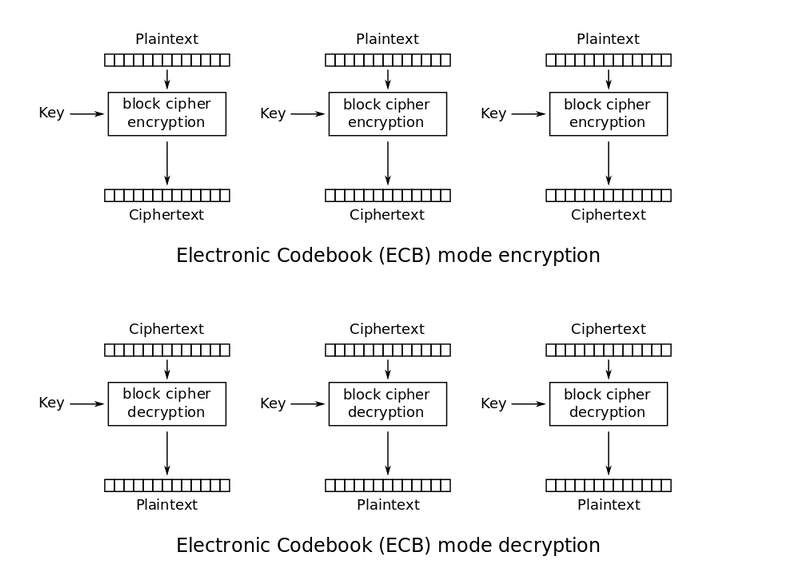
\includegraphics[scale=0.4]{imagenes/ecb.png} 
			\caption{Esquema del cifrado y descifrado del modo ECB \cite{cifradobloque}.}
			\label{esquemaecb}
		\end{figure}
		
	\item \textbf{Cipher-Block Chaining}\\
	En este modo se combina los bloques de texto plano con los bloques de texto cifrados anteriormente. Para cifrar el primer bloque será necesario un bloque inicial, $c_{[0]}$, el cual no tiene necesariamente que ser secreto. Los pasos seguidos para encriptar y desencriptar son:
	\begin{itemize}
		\item \textbf{\emph{Cifrado CBC}}
		\begin{description}
			\item $c_{[0]} \in \mathbb{B}^*$
			\item Dividimos m en $m_{[1]}\dots m_{[l]}$ con $m_{[i]} \in \mathbb{B}^N$
			\item Para $i\in\{1,\dots,l\}$ hacer
			\begin{description}
				\item $c_{[i]} = E_k(m_{[i]}\oplus c_{[i-1]})$
			\end{description}
			\item Devolvemos $c_{[1]}\dots c_{[l]}$
		\end{description}

		\item \textbf{\emph{Descifrado CBC}}
		\begin{description}
			\item Dividimos c en $c_{[0]}\dots c_{[l]}$ con $c_{[i]} \in \mathbb{B}^N$
			\item Para $i\in\{1,\dots,l\}$ hacer
			\begin{description}
				\item $m_{[i]} = D_k(c_{[i]})\oplus c_{[i]}$
			\end{description}
			\item Devolvemos $m_{[1]}\dots m_{[{l}]}$
		\end{description}
	\end{itemize}
\newpage
		\begin{figure}[htb]
			\centering
			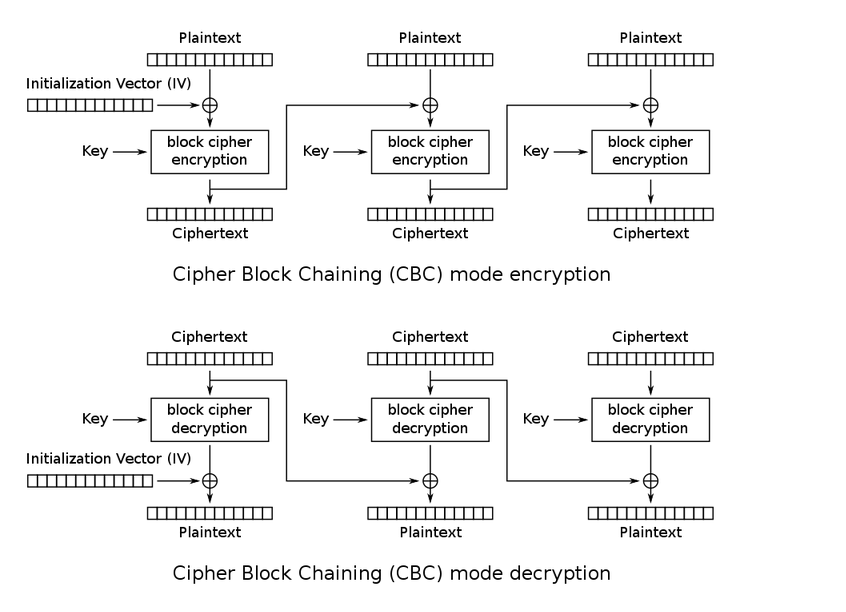
\includegraphics[scale=0.4]{imagenes/cbc.png} 
			\caption{Esquema del cifrado y descifrado del modo CBC \cite{cifradobloque}.}
			\label{esquemacbc}
		\end{figure}

	\item \textbf{Cipher FeedBack}\\
	Modo en el cual se combina cada bloque de texto plano del mensaje consigo mismo encriptado, los pasos que se siguen son:
	\begin{itemize}
		\item \textbf{\emph{Cifrado CFB}}
		\begin{description}
			\item $x_{[0]} \in \mathbb{B}^r$
			\item Dividimos m en $m_{[1]}\dots m_{[l]}$ con $m_{[i]} \in \mathbb{B}^N$
			\item Para $i\in\{1,\dots,l\}$ hacer
			\begin{description}
				\item $c_{[i]} = m_{[i]}\oplus msb_r(E_k(x_{[i]}))$
				\item $x_{[i+1]} = lsb_{N-r}(x_i)||c_{[i]$
			\end{description}
			\item Devolvemos $c_{[1]}\dots c_{[l]}$
		\end{description}

		\item \textbf{\emph{Descifrado CFB}}
		\begin{description}
			\item Dividimos c en $c_{[1]}\dots c_{[l]}$ con $c_{[i]} \in \mathbb{B}^r$
			\item Para $i\in\{1,\dots,l\}$ hacer
			\begin{description}
				\item $m_{[i]} = c_{[i]}\oplus msb_r(E_k(x_{[i]}))$
				\item $x_{[i+1]} = lsb_{N-r}(x_i)||c_{[i]$
			\end{description}
			\item Devolvemos $m_{[1]}\dots m_{[l]}$
		\end{description}
	\end{itemize}

%\newpage
		\begin{figure}[htb]
			\centering
			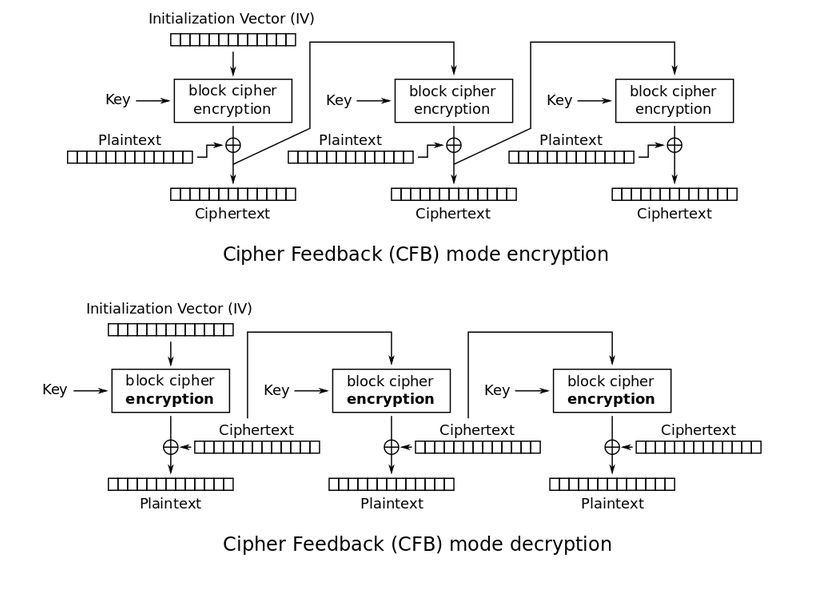
\includegraphics[scale=0.4]{imagenes/cfb.png} 
			\caption{Esquema del cifrado y descifrado del modo CFB \cite{cifradobloque}.}
			\label{esquemacfb}
		\end{figure}

\newpage
	\item \textbf{Output FeedBack}\\
	Modo en el cual se parte de un bloque inicial $x_{[0]}$ único y secreto. En cada iteración se encripta este y se combina con un bloque del mensaje sin cifrar de manera recursiva. Los pasos seguidos para encriptar y desencriptar son:
	\begin{itemize}
		\item \textbf{\emph{Cifrado OFB}}
		\begin{description}
			\item $x_{[0]} \in \mathbb{B}^N$
			\item Dividimos m en $m_{[1]}\dots m_{[l]}$ con $m_{[i]} \in \mathbb{B}^N$
			\item Para $i\in\{1,\dots,l\}$ hacer
			\begin{description}
				\item $x_{[i]} = E_k(x_{[i-1]})$
				\item $c_{[i]} = m_{[i]}\oplus x_{[i]}$
			\end{description}
			\item Devolvemos $c_{[1]}\dots c_{[l]}$
		\end{description}

%\newpage
		\item \textbf{\emph{Descifrado OFB}}
		\begin{description}
			\item Dividimos c en $c_{[1]}\dots c_{[l]}$ con $c_{[i]} \in \mathbb{B}^N$
			\item Para $i\in\{1,\dots,l\}$ hacer
			\begin{description}
				\item $x_{[i]} = E_k(x_{[i-1]})$
				\item $m_{[i]} = c_{[i]}\oplus x_{[i]}$
			\end{description}
			\item Devolvemos $m_{[1]}\dots m_{[l]}$
		\end{description}
	\end{itemize}
		\begin{figure}[htb]
			\centering
			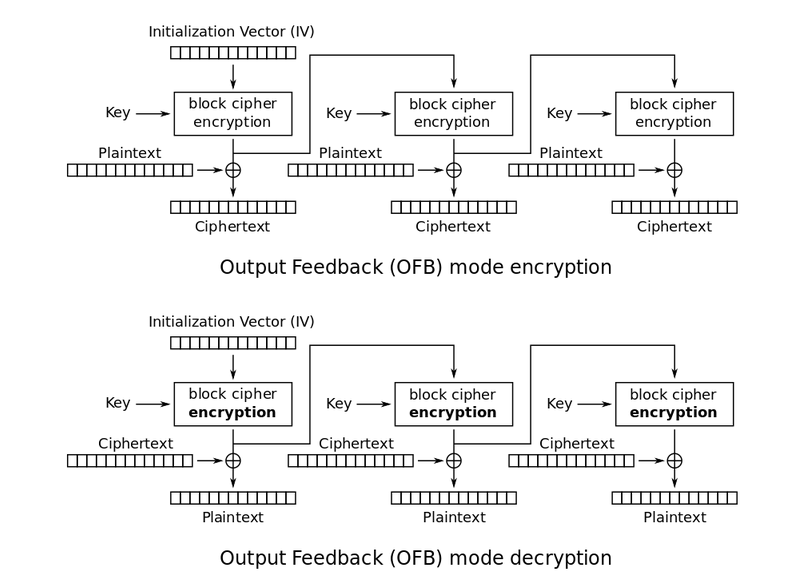
\includegraphics[scale=0.4]{imagenes/ofb.png} 
			\caption{Esquema del cifrado y descifrado del modo OFB \cite{cifradobloque}.}
			\label{esquemaofb}
		\end{figure}
\end{itemize}
\newpage
Como podemos ver, el más sencillo es ECB ya que lo único que hace es fragmentar el mensaje en bloques y encriptar individualmente cada bloque. En CBC, CFB y OFB se parte de un bloque inicial y se generan bloques nuevos de manera recursiva operando con ellos de manera disinta en fución de cada modo.\\ 
En CBC se realiza la operación $\oplus$ de cada bloque generado encriptandose el bloque cifrado previo a esta con un bloque del mensaje, los nuevos bloques son los resultados de la operación anterior.\\
En CFB se coge el bit menos significativo de resultado de encriptar el bloque generado previo y se hace la operación $\oplus$ con cada bloque del mensaje. Para generar un nuevo bloque se combina el mensaje cifrado previo con el bit menos significativo del conjunto de bits $N-r$ del bloque generado anterior con la operación $||$.\\
Y en OFB se realiza la operación $\oplus$ de el resultado de encriptar el bloque generado previo con un bloque del mensaje.\\
Actualmente el más utilizado en las aplicaciones de mensajería es el modo CBC. Esto es debido a que es relativamente fácil de implementar y además permite encriptar en paralelo.
\section{El algoritmo Rijndael AES}
En esta sección hablaré sobre el cifrado Rijndael AES el cual es un cifrado de bloque simétrico muy utilizado actualmente por aplicaciones como \emph{Telegram}, \emph{WhatsApp} y \emph{FacebookChat} entre otras.\\
El algoritmo Rijndael llamado así en honor a sus dos autores Joan Daemen y Vicent Rijmen, es un algoritmo de cifrado por bloques que fue adoptado en octubre de 2000 por el NIST (\emph{National Institute for Standards and Technology}) para su empleo en aplicaciones criptográficas no militares en sustitución del algoritmo \emph{DES} después de un proceso de más tres años en los que se buscaba un algoritmo que fuera potente, eficiente y fácil de implementar.\\
Está diseñado para manejar longitudes de clave y de bloque variables entre los 128 y los 256 bits y aunque estos sean variables, en el estándar adoptado por el Gobierno de Estados Unidos en 2001 \cite{aesUsa} establece una longitud fija de bloque de 128 bits y una longitud de clave a escoger entre 128, 192 y 256 bits.\\
La información para los siguientes apartados de AES la he obtenido de \cite{En2011}.\\

\subsection{Estructura de AES}
%\subsection{Elementos de AES}
AES es un algoritmo que se basa en aplicar un número determinado de rodas a un valor intermedio denominado \emph{estado} que puede ser representado por una matriz rectangular que posee cuatro filas y $N_{b}$ columnas. Análogamente la clave tiene la misma estructura, una matriz de cuatro filas y $N_{k}$.
El bloque a cifrar o descifrar se traslada directamente byte a byte sobre la matriz de estado de columna en columna($a_{0,0}, a_{1,0}, a_{2,0}, a_{3,0}, a_{0,1} ...$)

\begin{table}[htb]
	\begin{center}
		\begin{tabular}{| l | l | l | l |}
				\hline
				$\math{a}_{0,0}$ & $\math{a}_{0,1}$ & $\math{a}_{0,2}$ & $\math{a}_{0,3}$\\ \hline
				$\math{a}_{1,0}$ & $\math{a}_{1,1}$ & $\math{a}_{1,2}$ & $\math{a}_{1,3}$\\ \hline
				$\math{a}_{2,0}$ & $\math{a}_{2,1}$ & $\math{a}_{2,2}$ & $\math{a}_{2,3}$\\ \hline
				$\math{a}_{3,0}$ & $\math{a}_{3,1}$ & $\math{a}_{3,2}$ & $\math{a}_{3,3}$\\ \hline
		\end{tabular}
		\caption{Ejemplo de matriz de estado con $N_b=4$(128 bits).}
	\end{center}
\end{table}

\begin{table}[htb]
	\begin{center}
		\begin{tabular}{| l | l | l | l |}
				\hline
				$\math{k}_{0,0}$ & $\math{k}_{0,1}$ & $\math{k}_{0,2}$ & $\math{k}_{0,3}$\\ \hline
				$\math{k}_{1,0}$ & $\math{k}_{1,1}$ & $\math{k}_{1,2}$ & $\math{k}_{1,3}$\\ \hline
				$\math{k}_{2,0}$ & $\math{k}_{2,1}$ & $\math{k}_{2,2}$ & $\math{k}_{2,3}$\\ \hline
				$\math{k}_{3,0}$ & $\math{k}_{3,1}$ & $\math{k}_{3,2}$ & $\math{k}_{3,3}$\\ \hline
		\end{tabular}
		\caption{Ejemplo de clave con $N_k=4$(128 bits).}
	\end{center}
\end{table}

En otros casos el bloque y la clave pueden ser representados como vectores de registro de 32 bits donde cada registro esta compuesto por los bytes de la columna correspondiente ordenados en orden descendiente.\\

Siendo $B$ el bloque que queremos cifrar y $S$ la matriz de estado, el algoritmo AES con $n$ rondas quedaría:

\begin{enumerate}
	\item Calcular $K_0, K_1,...,K_n$ subclaves a partar de la clave $K$.
	\item $S\leftarrow B \oplus K_0$
	\item Para $i=1$ hasta $n$ hacer
	\begin{description}
			\item Aplicar la roda \emph{i}-ésima del algoritmo con la subclave $K_i$
	\end{description}
\end{enumerate}
Como las funciones usadas en cada ronda son invertibles, para descifrar aplicaremos las funciones inversas de las funciones usadas para cifrar en el orden opuesto.

\begin{table}[htb]
	\begin{center}
		\begin{tabular}{| l | l | l | l |}
				\hline
				& $N_b = 4$(128 bits) & $N_b = 6$(192 bits)& $N_b = 8$(256 bits)\\ \hline
				$N_k = 4$(128 bits)& 10 & 12 & 14\\ \hline
				$N_k = 6$(128 bits)& 12 & 12 & 14\\ \hline
				$N_k = 8$(128 bits)& 14 & 14 & 14\\ \hline
		\end{tabular}
		\caption{Número de rodas en función del tamaño de la clave y bloque}
		\label{rondas_aes}
	\end{center}
\end{table}


En el algoritmo AES se define cada ronda como una composición de cuatro funciones invertibles diferentes, formando tres \emph{capas}. Estas funciones tienen un propósito específico:
\begin{itemize}
	\item \textbf{Capa de mezcla lineal:} Formada por las funciones \emph{DesplazarFila} y \emph{MezclarColumnas} y permite obtener un alto nivel de difusión a lo largo de varias rondas.
	\item \textbf{Capa no lineal:} Formada por la función \emph{ByteSub} y es la aplicación paralela de s-cajas con propiedades óptimas de no linealidad.
	\item \textbf{Capa de adición de clave:} Es un simple \emph{or-exclusivo} entre el estado intermedio y la subclave correspondiente a cada ronda.
\end{itemize}

\subsection{El cuerpo de Galois $\operatorname{GF}(2^n)$}
Antes de desarrollar las rondas de AES y posteriormente la teoría de Curvas Elípticas en $\operatorname{GF}(2^n)$ introduciré el cuerpo $\operatorname{GF}(2^n)$ el cual tiene una serie de propiedades que lo hacen muy interesante y justifican su uso tan extendido en criptografía.\\
El conjunto $\mathbb{Z}_2[x]$ es el conjunto de polinomios con coeficientes en $\mathbb{Z}_2$ es decir, el el conjunto de polinomios cuyos coeficientes solo valen 0 o 1. Por lo que los polinomios pueden ser representados por una cadena de bits.
 Un ejemplo sería el polinomio $f(x)=x^4+x^3+x+1$ que quedaría representado como 11011. 
Además si lo sumamos con otro polinomio como puede ser $g(x)=x^2+x+1$ tenemos que $f(x)+g(x)=x^4+x^3+x^2$ que equivale a hacer la operación \emph{xor} entre 11011 y 00111, por lo que a nivel computacional, es muy fácil implementar estas operaciones.\\
Escogiendo un polinomio irreducible en $\mathbb{Z}_2$ podemos generar un cuerpo de Galois. Este conjunto es representado como $\operatorname{GF}(2^n)$, donde $n$ es el grado del polinomio irreducible que lo genera.\\
Las principales ventajas que tiene trabajar con $\operatorname{GF}(2^n)$ es que permite llevar a cabo implementaciones de una sencillez significativa respecto a la de los demás. Por lo que teniendo el mismo orden de complejidad, se multiplica significativamente la velocidad y además permite simplificar el diseño de los circuitos. Esto último hace que se obtengan sistemas con mejores prestaciones y mejor precio.

\subsection{Las Rondas de AES}
Dado que el algoritmo AES puede aplicarse para longitudes diferentes de bloque y clave, el número de rondas es variable, como se ha visto en \ref{rondas_aes}.\\
Siendo $S$ la matriz de estado y $K_i$ la subclave correspondiente a la ronda $i$-ésima, cada ronda posee esta estructura:
\begin{enumerate}
	\item $S \leftarrow ByteSub(S)$
	\item $S \leftarrow DesplazarFila(S)$
	\item $S \leftarrow MezclarColumnas(S)$
	\item $S \leftarrow K_i \oplus S$
\end{enumerate}
En la última ronda se hacen solo los tres primeros pasos del algoritmo.

\begin{description}
	\item \textbf{ByteSub}\\
		La función \emph{ByteSub} es una sustitución no lineal que se aplica a cada byte de la matriz de estado mediante una s-caja 8\texttimes8. Se obtiene componiendo dos transformaciones:
		\begin{enumerate}
			\item Cada byte se considera como un elemento del $\operatorname{GF}(2^8)$ generado por el polinomio irreducible $m(x)=x^8+x^4+x^3+x+1$ y es sustituido por su inversa multiplicativa quedando el valor cero inalterado. 
			\item A continuación se aplica la siguiente transformación afín en $\operatorname{GF}(2)$ siendo $x_0, x_1,...,x_7$ los bits del byte correspondiente e $y_0, y_1,...,y_7$ los del resultado:

				\begin{equation*} 
					\begin{bmatrix} 
						y_0\\
						y_1\\
						y_2\\
						y_3\\
						y_4\\
						y_5\\
						y_6\\
						y_7\\
					\end{bmatrix}
					=
					\begin{bmatrix} % O matrices como esta de 4 x 3
						1 & 0 & 0 & 0 & 1 & 1 & 1 & 1\\
						1 & 1 & 0 & 0 & 0 & 1 & 1 & 1\\
						1 & 1 & 1 & 0 & 0 & 0 & 1 & 1\\
						1 & 1 & 1 & 1 & 0 & 0 & 0 & 1\\
						1 & 1 & 1 & 1 & 1 & 0 & 0 & 0\\
						0 & 1 & 1 & 1 & 1 & 1 & 0 & 0\\
						0 & 0 & 1 & 1 & 1 & 1 & 1 & 0\\
						0 & 0 & 0 & 1 & 1 & 1 & 1 & 1\\
					\end{bmatrix}
					\begin{bmatrix}
						x_0\\
						x_1\\
						x_2\\
						x_3\\
						x_4\\
						x_5\\
						x_6\\
						x_7\\
					\end{bmatrix}
					+
					\begin{bmatrix}
						1\\
						1\\
						0\\
						0\\
						0\\
						1\\
						1\\
						0\\
					\end{bmatrix}
			\end{equation*}
		\end{enumerate}
		La función inversa de $ByteSub$ es la aplicación inversa de la s-caja de cada byte de la matriz de estado.

	\item \textbf{DesplazarFila}\\
		Esta función desplaza a la izquierda de manera cíclica las filas de la matriz de estado. Cada fila $f_i$ se desplaza un número de posiciones $c_i$ diferente. Mientras que $c_0$ siempre es igual a cero, el resto de valores vine en función de $N_b$ como se puede ver en \ref{ciennb}.\\
		La función inversa será el desplazamiento de las filas de la matriz el mismo número de posiciones pero en el sentido contrario.

		\begin{table}[htb]
			\begin{center}
				\begin{tabular}{| l | l | l | l |}
						\hline
						$N_b$ & $c_1$ & $c_2$ & $c_3$\\ \hline
						4 & 1 & 2 & 3\\ \hline 
						6 & 1 & 2 & 3\\ \hline 
						8 & 1 & 3 & 4\\ \hline 
				\end{tabular}
				\caption{Valores de $c_i$ según el tamaño de bloque $N_b$}
				\label{ciennb}
			\end{center}
		\end{table}

		\begin{figure}[htb]
			\centering
			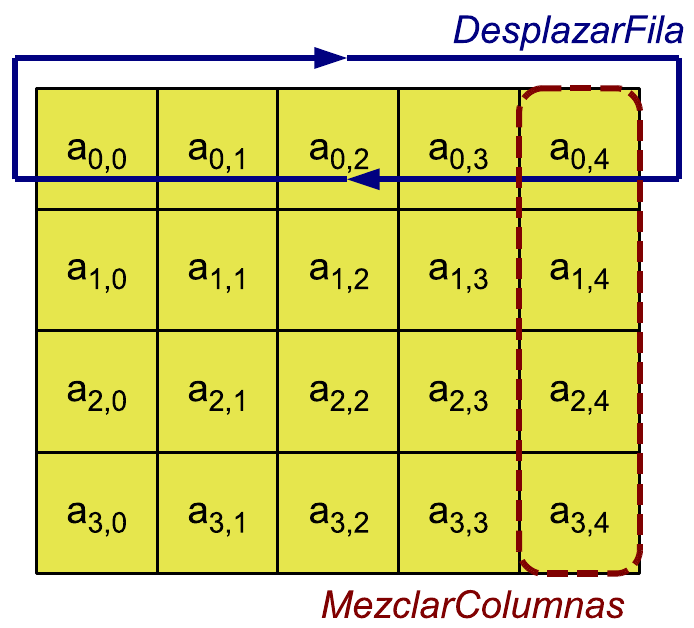
\includegraphics[scale=0.4]{imagenes/aesdesplazarmezclar.png} 
			\caption{Esquema de las funciones $MezclarColumnas$ y $DesplazarFila$ \cite{En2011}}
			\label{desplazarymezclar}
		\end{figure}
%\newpage
	\item \textbf{MezclarColumnas}\\
		Durante la aplicación de esta función se considera cada columna del vector de estado se considera un polinomio cuyos coeficientes pertenecen a $\operatorname{GF}(2^8)$ y se multiplica módulo $x^4+1$ por: $c(x)=03x^3+01x^2+01x+02$ donde 03 es el valor hexadecimal que se obtiene concatenado los coeficientes binarios del polinomio correspondiente en $\operatorname{GF}(2^8)$, en este caso sería 00000011 y por tanto $x+1$ análogamente se haría con los demás.\\
		La inversa de $MezclarColumnas$ se obtiene multiplicando cada columna de la matriz de estado por el polinomio: $d(x)=0Bx^3+0Dx^2+09x+0E$.

\end{description}

\subsection{Cálculo de las Subclaves}
Las subclaves $K_i$ se obtienen de la clave principal $K$ mediante el uso de dos funciones: una de expansión y otra de selección. Siendo $n$ el número de rondas que se van a aplicar, la función de expansión obtiene a partir del valor de $K$ una secuencia de $4(n+1)N_b$ bytes.\\
La función de selección toma consecutivamente de la secuencia obtenida bloques del mismo tamaño que la matriz de estado y los asigna a cada $K_i$.\\

Sea $K(i)$ un vector de bytes de tamaño $4N_k$ conteniendo la clave y sea $W(i)$ un vector de $N_b(n+1)$ registros de 4 bytes, siendo $n$ el número de rondas. 
La función de expansión tiene dos versiones según el valor de $N_k$:

\begin{itemize}
	\item Si $N_k<=6$:
	\begin{algorithm}
		Para $i$ desde 0 hasta $N_{k}-1$ hacer:
		\begin{description}
			$W(i)\leftarrow(K(4·i), K(4·i+1), K(4·i+2), K(4·i+3))$
		\end{description}
		Para $i$ desde $N_k$ hasta $N_{b}·(n+1)$ hacer:\\
			\hspace*{20}$tmp\leftarrow W(i-1)$\\
			\hspace*{20}Si $i$ $mod N_k = 0$\\
			\hspace*{40}$tmp\leftarrow Sub(Rot(tmp))\oplus Rc(i/N_k)$\\
			\hspace*{20}$W(i)\leftarrow W(i-N_k)\oplus tmp$
	\end{algorithm}

	\item Si $N_k>6$:
	\begin{algorithm}
		Para $i$ desde 0 hasta $N_{k}-1$ hacer:
		\begin{description}
			$W(i)\leftarrow(K(4·i), K(4·i+1), K(4·i+2), K(4·i+3))$
		\end{description}
		Para $i$ desde $N_k$ hasta $N_{b}·(n+1)$ hacer:\\
			\hspace*{20}$tmp\leftarrow W(i-1)$\\
			\hspace*{20}Si $i$ $mod N_k = 0$\\
			\hspace*{40}$tmp\leftarrow Sub(Rot(tmp))\oplus Rc(i/N_k)$\\
			\hspace*{20}Si $i$ $mod N_k = 4$\\
			\hspace*{40}$tmp\leftarrow Sub(tmp)$\\
			\hspace*{20}$W(i)\leftarrow W(i-N_k)\oplus tmp$
	\end{algorithm}
\end{itemize}

La función \emph{Sub} devuelve el resultado de aplicar la s-caja de AES a cada uno de los bytes del registro de cuatro que se le pasa como parámetro, la función \emph{Rot} desplaza a la izquierda los bytes del registro y \emph{Rc(j)} es una constante que se define como:
\begin{itemize}
	\item $Rc(j)=(R(j),0,0,0)$.
	\item Cada $R(i)$ es el elemento de $\operatorname{GF}(2^8)$ correspondiente al valor $x^{i-1}$ módulo $x^8+x^4+x^3+x+1$.
\end{itemize}

\section{Criptosistema de Rivest-Shamir-Adleman, RSA}
En esta sección hablaré sobre el cifrado RSA y su funcionamiento, cifrado que como AES, está muy extendido y es utilizado por muchas aplicaciones para cifrar y validar los mensajes.\\
RSA es llamado así en honor a sus creadores Ron Rivest, Adi Shamir y Loenard Adleman, fué desarrollado en 1977. Cabe a destacar que en 1973 se desarrolló en secreto un criptosistema similar por Clifford Cocks para la \emph{Government Communications Headquarters}, que es la agencia de inteligencia de señales británica, y fue desclasificado en 1997\cite{cliffordCocks}.\\
Este criptosistema está basado en el \emph{Teorema de Euler} y en particular en la \emph{Proposición 2.2}.\\

\begin{teorema}
	(Teorema pequeño de Fermat) Sea $a \in \mathbb{Z}$ y $p$ un número primo tal que $mcd(a,p)=1$. Entonces
	$$
		a^{p-1} \equiv 1 \mod p.
	$$
\end{teorema}\vspace*{-10mm}
\begin{proof}
		Sea $a \in \mathbb{Z}$. Tomamos los $p-1$ primeros múltiplos positivos de $a$ que serán de la forma $a, 2a,\dots,(p-1)a$. El resto resultante de dividir los $p-1$ múltiplos positivos de $a$ por $p$ corresponden a 1,2,3,$\dots,p-1$.\\
	Multiplicando ahora todas las congruencias obtenemos 
	$$
		a^{p-1}·(p-1)! \equiv (p-1)! \mod p.
	$$
	Como tenemos que $p\nmid (p-1)!$ se cumple que $mcd(p,p-1)=1$ y por tanto cancelando en la expresión anterior obtenemos
	$$
		a^{p-1} \equiv 1 \mod p.
	$$
\end{proof}

\begin{teorema}
	(Teorema de Euler) Sean a,n $\in \mathbb{Z}$ primos relativos entre sí, entonces $a^{\phi(n)}\equiv 1 \mod n$.
\end{teorema}\vspace*{-10mm}
\begin{proof}
		Sea $n\in \mathbb{Z^+}$ que verifica que $mcd(a,n)=1$ y definimos $S$ como el conjunto de las unidades modulo $n$, $S=\{u_1,u_2,\dots,u_{\phi(n)}\}$ donde $1\leq u_i\leq n-1$, $mcd(u_i,n)=1$ y $u_i\neq u_j$ $\forall i,j \in \{1,\dots,\phi(n)\}$ con $ i\neq j$.\\
	Multiplicando  los elementos de $S$ por $a$ obtenemos 
	$$
		aS=\{au_1,au_2,\dots,au_{\phi(n)}\}
	$$
	Como $mcd(a,n)=1$ entonces $a\mod n$ es una unidad y por tanto $aS$ será el conjunto de las unidades módulo $n$. Y dado que los elementos de $S$ y los de $aS$ coinciden módulo $n$, el producto de estos será el mismo módulo $n$ por lo que obtenemos 
	$$
		u_1u_2\dots u_{\phi(n)} \equiv (au_1)(au_2)\dots (au_{\phi(n)})\mod n.
	$$
	Sacando como factor común $a$ tenemos 
	$$
		u_1u_2\dots u_{\phi(n)} \equiv a^{\phi(n)}u_1u_2\dots u_{\phi(n)}\mod n.
	$$
\end{proof}\\
Donde $\phi(n)$ es la \emph{funclón de Euler} definida como $\phi(n)=|\mathbb{Z}^*_n|$ y se puede calcular de la siguiente forma $$\phi(n)=n\prod_{p_i|n}\left(1-\frac{1}{p_i}\right).$$

\begin{teorema}
		(Teorema Chino del Resto) Sean $a_i\in \mathbb{Z}$ y $p,q \in \mathbb{N}$ tales que $mcd(p,q)$ con $i = 1,2$. Entonces el sistema
		$$
			x\equiv a_1 \mod p,
		$$\vspace*{-10mm}

		$$
			x\equiv a_2 \mod q,
		$$

	tiene solución única módulo $n=pq$. Además, la solución está dada por
	$$
		x\equiv a_1\cdot c_1\cdot d_1 +a_2\cdot c_2\cdot d_2 \mod n,
	$$
	donde se cumple
	$$
		c_1=\frac{n}{p},
	$$
	$$
		c_2=\frac{n}{q},
	$$
		y
	$$
		c_1\cdot d_1 \equiv 1 \mod p,
	$$
	$$
		c_2\cdot d_2 \equiv 1 \mod q.
	$$
	
\end{teorema}

\begin{proposicion}
	Sea $n = pq$, donde p y q son dos primos distintos. Si $x\equiv 1 \mod \phi(n)$, entonces $a^x\equiv a\mod n$ para todo $ a \n \in \mathbb{Z}$.
\end{proposicion}\vspace*{-10mm}
	\begin{proof}
		Si $a$ es múltiplo de $n$, entonces se cumple que $a^x \equiv 0 \equiv a \mod n$. Si $a$ y $n$ son coprimos, $mcm(a,n) = 1$. Entonces tendríamos que $a^x \equiv a \mod n$ por el Teorema de Euler.\\
		Nos quedaría ver ocurre en el caso de $a$ sea múltiplo de $p$ o de $q$, pero no de ambos. Por simetría supondremos que a es múltiplo de $p$, pero no de $q$. En este caso tenemos que $a^x \equiv 0 \equiv a \mod p$  y $a^x \equiv a \mod q$ por el Teorema de Fermat. Como $p$ y $q$ son coprimos entre sí, aplicando el Teorema Chino del Resto se deduce que $a^x \equiv a \mod n$.
	\end{proof}

\subsection{Descripción de RSA}
El contenido de esta sección se basa en \cite{angelRiosMateos}. El funcionamiento de RSA es el siguiente.\\
El usuario elige dos números primos distintos \emph{p} y \emph{q} de buen tamaño ya que mientras más grandes sean más seguro será el cifrado.
Se calcula $n = pq$ y por tanto tenemos que $\phi(n) = (p-1)(q-1)$. A continuación se elige un elemento $c$ coprimo con $\phi(n)$ y se calcula el inverso $d = c^{-1}\mod \phi(n)$. La clave pública será $k=(n,c)$ y la clave privada $k'=(n,d)$.\\
En un principio se consideraba que un tamaño de $n$ de 1024 bits era lo suficientemente grande para que fuera seguro, pero en 2003 Tromer y Shamir mostraron que es posible factorizar números de 1024 bits \cite{1024RSA} por lo que en la actualidad se considera 2048 bits como un tamaño seguro.\\
El conjunto de los mensajes sin cifrar es $\mathcal{M}$, el de los mensajes cifrados será $\mathcal{C}$ y se verifica que $\mathcal{M} = \mathcal{C} = \mathbb{Z}_n$. Las funciones de cifrado y descifrado son respectivamente:
\begin{align*}
	E_{k}:\mathcal{M}\rightarrow\mathcal{C},\\
	a \rightarrow a^c,
\end{align*}
\begin{align*}
	D_{k'}:\mathcal{C}\rightarrow\mathcal{M},\\
	a \rightarrow a^d.
\end{align*}

\subsection{Ataques}
Como hemos visto anteriormente RSA puede ser vulnerable en función de los números primos que se elijan y el tamaño de estos. En este apartado veremos algunos posibles ataques que se podrían llevar a cabo \cite{apuntesCriptografia}.
	\subsubsection{Ataque por módulo común.}
	Este ataque se da cuando hay una mala elección de las claves, típicamente cuando se tienen que generar múltiples claves para varios usuarios y para optimizar, se utiliza el mismo módulo $n$ para todos. Mientras el exponente sea distinto, la clave sigue siendo segura, pero si se da que se cifra el mismo mensaje con los distintos exponentes pero el mismo módulo, se puede descifrar el mensaje original.\\
	Supongamos que tenemos dos claves públicas con el mismo módulo, $(n, e_1)$ y $(n, e_2)$ y además ser verifica que  $mcm(e_1,e_2)$. Supongamos que $re_1+se_2=1$ con $r$\textless $0$\textless $s$. Como se ha visto el mensaje cifrado respectivamente será:
	\begin{align*}
		c_1 = m^{e_1} \mod n\\
		c_2 = m^{e_2} \mod n
	\end{align*}
	Si $(c_1,n) \neq 1$, podemos factorizar $n$ y romper la clave, por lo que podemos suponer que $c_1 \in \mathcal{U}(\mathbb{Z}_n)$. Calculamos $c_1^{-1}$ con el algoritmo extendido de Euclídes tenemos que:
	\begin{align*}
			(c^{-1})^{-r}c_2^s \equiv (m^{e_1})^r(m^{e_2})^s \equiv m^{e_1r+e_2s} = m \mod n.
	\end{align*}

	\subsubsection{Ataque por exponente pequeño.}
	Este ataque se puede hacer cuando se elige un exponente muy pequeño y se cifra el mismo mensaje con distinto módulo. En este caso se puede recuperar el mensaje principal aplicando el Teorema Chino del Resto. Supongamos a varios receptores con claves públicas $(n_i, e)$, con $1\leq i \leq r$, tal que mcd$(n_i, n_j) = 1$ si $i\neq j$ ya que en caso contrario, se podría factorizar el módulo correspondiente mediante el cálculo del MCD.\\
	Llamamos $c_i = m^e \mod n_i$ para cada $1\leq i \leq r$. Seleccionamos $\{i_1,...,i_e \}\subseteq \{1,...,r\}$ y empleando el inverso del isomorfismo de anillos
	\begin{align*}
		\chi:\mathbb{Z}_{n_{i_1}\dots n_{i_e}}\rightarrow \mathbb{Z}_{n_{i_1}}\times \dots \times \mathbb{Z}_{n_{i_e}}
	\end{align*}
	obtenido gracias al Teorema Chino del Resto, se puede calcular
	\begin{align*}
		\chi^{-1}(c_{i_1},\dots,c_{i_e}) = m^e \mod n_{i_1},\dots,n_{i_e}
	\end{align*}
	Dado $m^e$\textless $n_{i_1}\dots n_{i_e}$, se puede obtener $m$ calculando la raíz $e$-ésima en $\mathbb{Z} \subseteq \mathbb{R}$, siempre y cuando $e$ no sea muy grande.

	\subsubsection{Ataque con primos muy próximos.}
	Este ataque se da cuando se eligen dos primos muy próximos entre sí. Dado $n=pq$, con $p$\textless $q$, tenemos que  
	\begin{align*}
			n=\left (\frac{p+q}{2}\right )^2-\left (\frac{p-q}{2}\right )^2.
	\end{align*}
	Si $p$ y $q$ son cercanos, $s=\frac{p-q}{2}$ es pequeño y $t=\frac{p+q}{2}$ es un entero ligeramente mayor que $\sqrt{n}$ tal que $t^2 - n^2$ es un cuadrado perfecto. Probando sucesivamente con valores mayores que $\sqrt{n}$ hasta encontrar una descomposición $n=t^2-s^2$, tenemos que $p=t+s$ y $q=t-s$.

\subsection{Firma digital RSA}
La firma digital con RSA, es una herramienta muy utilizada en las aplicaciones de mensajería para garantizar el no repudio de los mensajes.
Dados dos interlocutores A y B cada uno con sus claves públicas:
\begin{itemize}
	\item para A tenemos $n_A$, $d_A$ y $e_A$,  
	\item para B tenemos $n_B$, $d_B$ y $e_B$.  
\end{itemize}
Para que B sepa que un mensaje \emph{m} ha sido enviado por A se siguen los siguientes pasos:
\begin{enumerate}
	\item A cifra el mensaje \emph{m} usando su clave secreta:
		$$
			S=D_A(m)=m^{d_A} \mod n_A.
		$$
	\item A continuación encripta el mensaje firmado con la clave pública de B:
		$$
			C_B(S)=S\mod n_B.
		$$
		y se lo envía a B.
	\item B recibe $C_B(S)=S^{e_B}$ y lo desencripta: 
		$$
			D_B(S^{e_B})=S \mod n_B.
		$$
	\item Una vez desencriptado la primera parte, B desencripta S con la clave pública de A:
		$$
			C_A(S)=C_A(D_A(m))=(m^{d_A})^{e_A}=m^{d_Ae_B}=m^{1+k\phi(n_A)}\equiv m \mod n_A.
		$$
\end{enumerate}
Una vez hecho esto, B podría afirmar casi con total seguridad que el mensaje ha sido enviado por A garantizando el no repudio del mensaje.

\section{El Problema del Logaritmo Discreto. Diffie-Hellman}
El intercambio de claves \emph{Diffie-Hellman} es un método basado en el Problema del Logaritmo Discreto muy utilizado en las aplicaciones de mensajería al iniciar una conexión. La información de este apartado sobre el logaritmo ha sido obtenida de \cite{angelRiosMateos} y la de \emph{Diffie-Hellman} ha sido obtenida de \cite{En2011}.\\
El Problema del Logaritmo Discreto es definido de la siguiente forma:
\begin{definicion}
	Sea S un semigrupo finito. El Problema del Logaritmo Discreto en el semigrupo S es el de resolver ecuaciones del tipo\\
		$$
			a^x\!=b\;(x\in \mathbb{N}).
		$$
	donde a y b son dos elementos dados de S.
\end{definicion}

La complejidad del Problema del Logaritmo Discreto depende en gran medida del semigrupo $S$ que se elija.
Dado que si se eligiera como $S$ el grupo aditivo $\mathbb{Z}_n$ la solución se obtendría fácilmente resolviendo una ecuación de congruencias del tipo $aX \equiv b \mod n$ que equivaldría a resolver la ecuación diofántica $aX + nY = b$. Pero si ahora $S$ pasara a ser los semigrupos multiplicativos $\mathbb{Z}_n$ o $\mathbb{F}_q$ o sus grupos de unidades, el problema aumentaría su complejidad de manera significativa.\\
Tenemos que $a^x = b$ tiene solución si y solamente si $b$ está en el semigrupo cíclico generado por $a$. Luego si $a$ es un elemento de orden finito de un grupo, se podría suponer en la práctica que $S$ es un grupo cíclico y por ello existiría un isomorfismo con ($\mathbb{Z}_n$, $+$). Luego la dificultad del problema no estaría en la estructura del grupo, sino en reconocer los elementos como potencias de enteros.\\
Se cree que el problema de logaritmo discreto es $\mathbb{NP}$-completo, pero esta conjetura todavía no ha sido demostrada por lo que se considera un problema $\mathbb{NP}$-Intermedio, estos problemas son llamados así porque no están dentro de los problemas $\mathbb{P}$ ni en los problemas $\mathbb{NP}$-completo por ahora \cite{NP-intermedio}.\\
Una vez visto el problema de logaritmo discreto, se explicará el intercambio de claves \emph{Diffie-Hellman}.
\subsection{Intercambio de claves Diffie-Hellman}
Antes de explicar el intercambio de claves \emph{Diffie-Hellman} se introducirá el problema de Diffie-Hellman ya que es la base de este.\\

\begin{definicion}
	Dado el conjunto $\mathbb{Z}^*_{p'}$ con p primo, diremos que $\alpha \in \mathbb{Z}^*_p$ es un generador de $\mathbb{Z}^*_{p'}$ si se cumple:\\
	$$
		\forall b \in \mathbb{Z}^*_{p'},\: \exists i\: tal \: que \: \alpha^i = b
	$$
\end{definicion}

\begin{definicion}
	(El Problema Diffie-Hellman)\\ Dado un número primo p, un número $\alpha$ que sea un \emph{generador} de $\mathbb{Z}^*_{p'}$, $\alpha^a$ y $\alpha^b$, encontrar $\alpha^{ab} \mod p$.  
\end{definicion}

\subsubsection{Intercambio de claves \emph{Diffie-Hellman}}
El intercambio de claves \emph{Diffie-Hellman} es un algoritmo asimétrico basado en el problema de \emph{Diffie-Hellman}, empleado para acordar una clave común en un canal inseguro. Los pasos que se siguen son:\\
Sean $A$ y $B$ dos interlocutores que quieren compartir un valor $K$. Para ello se calcula un número primo $p$ y un generador \alpha de $\mathbb{Z}^*_{p'}$ con $2\leq \alpha \leq p-2$. Esta información es pública y conocida por ambos.
\begin{enumerate}
	\item $A$ escoge un número aleatorio $x$, comprendido entre 1 y $p-2$ y envía a $B$ el valor 
		$$
			\alpha^x \mod p
		$$
	\item Análogamente $B$ escoge un número aleatorio $y$, comprendido entre 1 y $p-2$ y envía a $A$ el valor 
		$$
			\alpha^y \mod p
		$$

	\item $B$ recoge $\alpha^x$ y calcula $K=(\alpha^x)^y \mod p$
	\item $A$ recoge $\alpha^y$ y calcula $K=(\alpha^y)^x \mod p$
\end{enumerate}
Puesto que $x$ e $y$ son conocidos solamente por $A$ y $B$ respectivamente, tenemos que al final solamente $A$ y $B$ acaban conociendo el valor de $K$.\\
A continuación se introducirá la teoría de curvas Elípticas ya que nos permitirá redefinir el intercambio de claves usando estas, generando un problema mucho más complejo y con mayor seguridad el cual es el que se utiliza en aplicaciones de mensajería como \textbf{WhatsApp} y \textbf{Telegram}.

\section{Curvas Elípticas en Criptografía}
La criptografía en curvas Elípticas es considerada como uno de los campos de las matemáticas con más futuro en la criptografía asimétrica.
Esto es debido a sus propiedades que dan lugar a problemas de una gran complejidad computacional análogos a los que presenta la aritmética modular. 
Esto permite que sean utilizadas en algunos algoritmos asimétricos como puede ser el intercambio de claves \emph{Diffie-Hellman} que se verá más adelante. A priori su 
estructura algebraica es más compleja que la de la aritmética modular sin embargo, al implementarlas suelen ser más eficientes y además, con claves más cortas alcanzan 
el mismo nivel de seguridad.\\
El uso de curvas elípticas en criptografía se presentó por primera vez en 1985 por Neal Koblitz y Víctor Miller de manera independiente.\\
La información para esta sección se ha obtenido de \cite{En2011}.

\subsection{Curvas Elípticas en $\mathbb{R}$}
\begin{definicion}
	Una curva definida en $\mathbb{R}$ es el conjunto de puntos del plano (x,y) que cumplen la siguiente ecuación:
$$
	y^2=x^3+ax+b
$$
Donde los coeficientes a,b $\in \mathbb{R}$ defininen de manera unívoca a la curva.
\end{definicion}
Algunas curvas en $\mathbb{R}$ son:

\begin{figure}[H]
	\centering
	\subfloat[\centering Curva $y^2=x^3-4x+1$]{{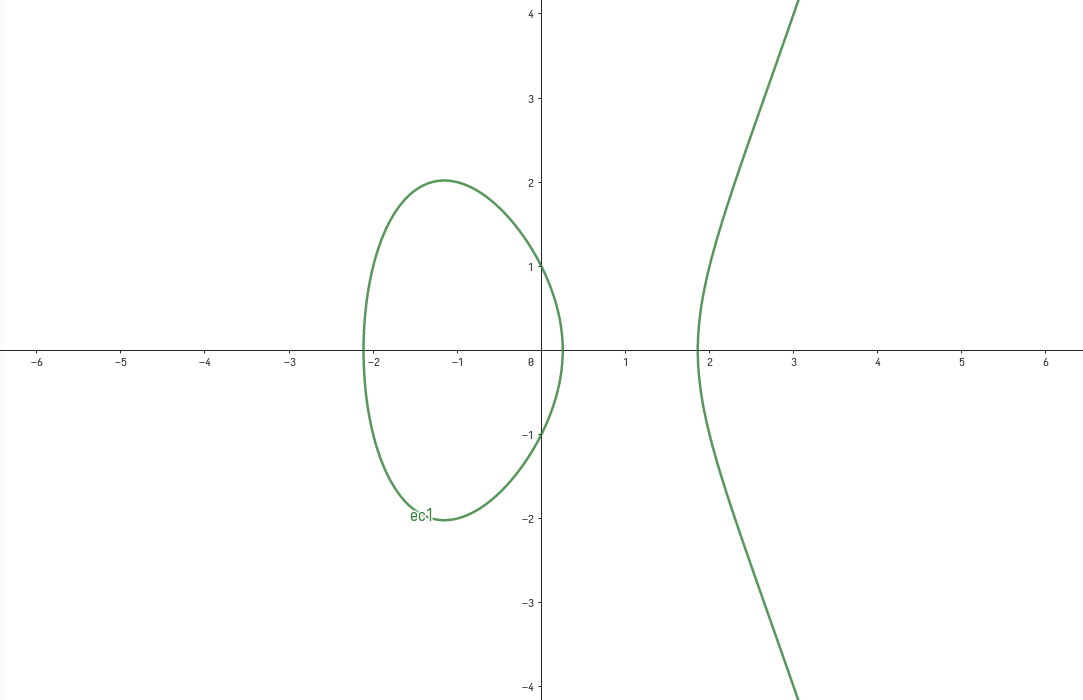
\includegraphics[width=5.9cm]{imagenes/ec1:y^2x^3-4x+1.png}}}
	\qquad
	\subfloat[\centering Curva $y^2=x^3-3x+4$]{{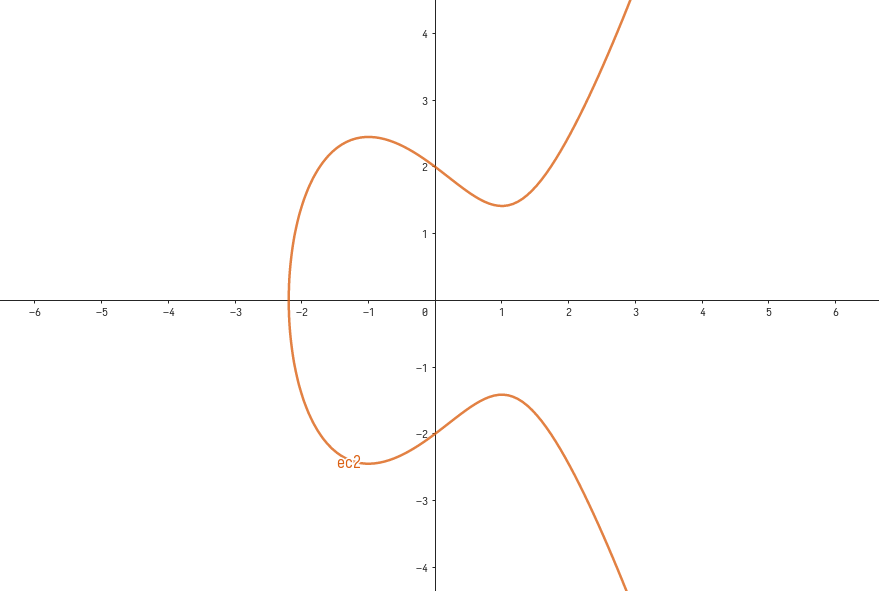
\includegraphics[width=5.9cm]{imagenes/ec2:y^2x^3-3x+4.png}}}
\end{figure}

Si se verifica que $x^3+ax+b$ no tiene raíces múltiples, tendremos que la curva junto con 
el punto $\mathcal{O}$ llamado \emph{punto en el infinito} y la operación $+$ que se definirá 
a continuación es lo que se denomina el \emph{grupo de curva elíptica E(\mathbb{R})}.\\
El punto $\mathcal{O}$ es un punto imaginario situado a una distancia infinita que no tendrá ningún valor en particular.\\

\textbf{Operación $+$ en $\mathbb{R}$}\\
Definido el conjunto en el que se trabajará, definiremos una ley de composición interna $+$.\\
Sean los puntos $r=(r_x,r_y)$, $s=(s_x,s_y)$, $p=(p_x,p_y)$, $t=(t_x,t_y)$ con $r,s,p,t \in E(\mathbb{R})$ la operación $+$ se define como sigue:
\begin{itemize}
	\item $r+\mathcal{O} = \mathcal{O}+r=r,\:\: \forall r \in E(\mathbb{R})$ .
	\item Si $r_x = s_x$ y $r_y = -s_y$, entonces $r=-s$ y además $r+s=s+r=\mathcal{O}$.
	\item Si $r\neq s$ y $r\neq -s$, $r+s=p$ donde $p$ será el opuesto del punto que corta la recta que une $r$ y $t$ con la curva.
	\item Para sumar un punto $p$ con sigo mismo si $p_y\neq0$ se usa la tangente de la curva en $p$. Luego tendremos que $t=p+p$ sera el opuesto de ese punto. Si $p_y=0$ entonces la tangente de la curva será perpendicular al eje de abcisas, por lo que se podría considerar que corta la curva en el infinito, luego $p+p=\mathcal{O}$.
	\item Para sumar $n$ veces un punto $p$ tenemos que si $p_y\neq 0$ entonces sumar $n$ veces $p$ será equivalente a multiplicar $p$ por el escalar $n$ y se representará como $np$. Si $p_y=0$ entonces la suma será:
\end{itemize}
\begin{aligned*}
	\center
	&$2r = r + r = \mathcal{O}$\\
	&$3r = 2r + r = \mathcal{O} + r = r$\\
	&$4r = 3r + r = r + r = \mathcal{O}$\\
	&...\\
\end{aligned}
La suma de curvas elípticas de manera algebraica se define de la siguiente forma:\\
Dados $r=(r_x,r_y)$ y $s=(s_x,s_y)$, tal que $r\noeq-s$, tenemos que $r+s=t$ donde $d=\frac{r_y-s_y}{r_x-s_x},\; t_x=d^2-r_x-s_x,\; t_y=-r_y+d(r_x-t_x)$.
De manera gráfica quedaría de la siguiente manera:\\
\begin{figure}[H]
	\centering
	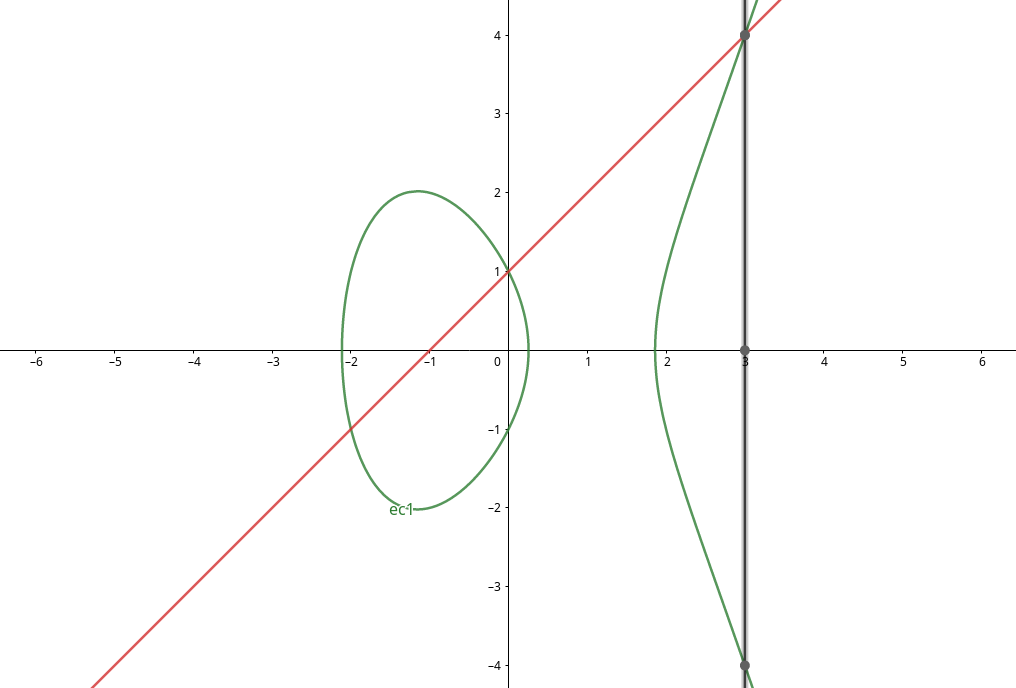
\includegraphics[scale=0.4]{imagenes/sumaCurva.png} 
	\caption{Suma en la curva $y^2=x^3-4x+1$ con $r=(-2,-1),\: s=(0,1),\: -t=(3,4)\: y \: t=(3,-4)$ }
	\label{esquemaecb}
\end{figure}

Una vez definidas las curvas elípticas en $\mathbb{R}$ definiremos las curvas en los cuerpos de Galois $\operatorname{GF}(n)$ y $\operatorname{GF}(2^n)$ cuyo uso esta muy extendido en la criptografía para redefinir el problema de logaritmo discreto.

\subsection{Curvas Elípticas en $\operatorname{GF}(n)$}
Un cuerpo de Galois $\operatorname{GF}(n)$ es el grupo finito generado por un número primo $n$. En este conjunto todos los elementos tienen un inverso, menos el cero por lo que están permitidas las operaciones de suma, resta, multiplicación y división.\\
De manera natural se define el conjunto $E(\operatorname{GF}(n))$ como los puntos $(x,y)$ que verifican la siguiente ecuación: 
$$
	y^2\equiv x^3+ax+b \mod n
$$
Donde al igual que en $E(\mathbb{R})$, $a,b\in{1..n}$ definen de manera unívoca una curva elíptica.\\

%\newpage
\subsubsection{Operación $+$ en $\operatorname{GF}(n)$}
Sean los puntos $r=(r_x,r_y),\: s=(s_x,s_y),\: p=(p_x,p_y),\: t=(t_x,t_y)\in E(\operatorname{GF}(n))$, definimos la operación $+$  como sigue:
\begin{itemize}
	\item $r+\mathcal{O}=\mathcal{O}+r=r,\: \forall r \in \operatorname{GF}(n)$.
	\item Si $r_x=s_x$ y $r_y=s_x+s_y$, entoces se dice que $r$ es el opuesto de $s$, se nota como $r=-s$ y se verifica que $r+s=s+r=\mathcal{O}$.
	\item Si $r\neq s$ y $r\neq-s$, $t=r+s$ se calcula como $d=\frac{s_y-r_y}{s_x-r_x}\mod n,\; t_x=d^2-r_x-s_x \mod n,\; t_y=-r_y+d(r_x-t_x) \mod n$
	\item Si $p_x = 0$ entonces $2p = \mathcal{O}$
\end{itemize}

\subsection{Curvas Elípticas en $\operatorname{GF}(2^n)$}

De manera análoga a $E(\operatorname{GF}(n))$ definimos el conjunto $E(\operatorname{GF}(2^n))$ con la diferencia debida a la estructura de $\operatorname{GF}(2^n)$, la ecuación de curva elíptica es diferente.\\
Dado un polinomio irreducible $p(x)$ de grado $n$, las curvas elípticas se definen como los puntos $(x,y)$ que cumplen la ecuación:
$$
	y^2+xy \equiv x^3+ax^2+b \mod (p(x))
$$
y para que se genere un grupo se tiene que verificar que $b\neq 0$.
Los puntos de una curva serán pares de polinomios de grado $n-1$ y como hemos visto en el apartado anterior, podrán ser representados como cadenas de bits.\\

\subsubsection{Operación $+$ en $E(\operatorname{GF}(2^n))$}
Sean los puntos $r=(r_x,r_y),\: s=(s_x,s_y),\: p=(p_x,p_y),\: t=(t_x,t_y)\in E(\operatorname{GF}(n))$, definimos la operación $+$  como sigue:
\begin{itemize}
	\item $r+\mathcal{O}=\mathcal{O}+r=r,\; \forall r \in E(\operatorname{GF}(2^n))$
	\item Si $r_x=s_x$ y $r_y=s_x+s_y$, entoces se dice que $r$ es el opuesto de $s$, se nota como $r=-s$ y se verifica que $r+s=s+r=\mathcal{O}$.
	\item Si $r\neq s$ y $r\neq-s$, $t=r+s$ se calcula como $d=\frac{s_y-r_y}{s_x-r_x},\; t_x=d^2+d+r_x+s_x+a,\; t_y=d(r_x+t_x)+t_x+r_y$.
	\item Para $t=2p$ con $p_x\neq 0$ se calcula como $d=p_x+\frac{p_y}{p_x}, \: t_x=d^2+d+a, \: t_y=p_x^2+(d+1)t_x$.
	\item Si $p_x=0$ tenemos que $2p=\mathcal{O}$
\end{itemize}

\section{El problema del logaritmo discreto usando curvas elípticas. \emph{Diffie-Hellman}}
En esta sección se hablará sobre el análogo del problema del logaritmo discreto en curvas elípticas y como resultado un análogo del intercambio de claves \emph{Diffie-Hellman}.

\subsection{El problema del logaritmo discreto en curvas elípticas}
Para todo punto $p$ definido en una curva elíptica, se define $\langle p\rangle$ al conjunto $\{\mathcal{O}, p, 2p, ... \}$.
En $E(\operatorname{GF}(n))$ y $E(\operatorname{GF}(2^n))$ los conjutos como los que se han definido, tienen que ser finitos ya que los puntos de las curvas son finitos. Luego para todo punto $q\in \langle p\rangle$ tiene que existir un númer $k \in \mathbb{Z}$ que verifique que $kp=q$.\\
Por lo tanto, el problema del logaritmo discreto en curvas elípticas consiste en hallar dicho número $k$ a partir de $p$ y $q$.
\subsection{Intercambio de claves \emph{Diffie-Hellman} en curvas elípticas}
Una vez visto el problema del logaritmo discreto en curvas elípticas, se explicará el intercambio de claves $Diffie-Hellman$ usando curvas elípticas. Para ello se explicará previamente la conjetura \emph{Diffie-Hellman}. La información de este apartado la he obtenido de \cite{apuntesCriptografia}.\\
Fijamos una curva elíptica $E=E(a,b)$ tal que $|E|=hn$ con $n$ primo y $h$ pequeño. Se fija también $q$ un elemento de orden $n$.
\begin{definicion}
	(Conjetura Diffie-Hellman). Conocidos $p_a=aq$ y $p_b=bq$ para ciertos $1\leq a,\: b\leq n$, calcular $abq$ es equivalente a nivel computacional a calcular $a=\log_q(p_a)$ o $b=\log_q(p_b)$.
\end{definicion}
El protocolo de intercambio de claves queda como:\\

Dadas dos personas A y B que quieren realizar un intercambio de claves.
\begin{itemize}
	\item A y B se ponen de acuerdo en la curva elíptica $E$ y el punto $q\in E$.
	\item A elige aleatoriamente un número $a\in(2,...,n-1)$ y le envía a B $p_a=aq$.
	\item B elige aleatoriamente un número $b\in(2,...,n-1)$ y le envía a A $p_b=bq$.
	\item A calcula $a(p_b)$.
	\item B calcula $b(p_a)$.
	\item La clave compartida es $(ab)q=a(p_b)=b(p_a)$
\end{itemize}

\section{Funciones Hash}
Una función resumen o función hash es un proceso en el cual se transforma un conjunto arbitrario de datos en una nueva serie de caracteres con una longitud fija independiente del tamaño de los datos de entrada, la información para esta sección la he obtenido \cite{aepd}.\\
Las propiedades esperadas de una función hash son:
\begin{itemize}
	\item Se tiene que poder utilizar en contenido digital de cualquier tamaño y formato.
	\item Independientemente del tamaño de la entrada y del tipo, se produce una salida numérica de tamaño fijo.
	\item Para el mismo conjunto de datos de entrada, el resultado siempre es el mismo.
	\item Reconstruir el mensaje original a partir del generado tiene que ser muy complejo, idealmente imposible.
	\item Una variación mínima del mensaje original tiene que producir un hash totalmente distinto, esta propiedad se denomina \emph{difusión}.
	\item Dado un mensaje, tiene que ser muy difícil encontrar otro mensaje con la misma imagen que este \emph{colisión débil}.
	\item Tiene que ser muy costoso encontrar dos mensajes que tengan la misma imagen, esta propiedad es denominada \emph{colisión fuerte}.
	\item Dado un posible valor del espacio imagen, tiene que ser igual de probable que salga este u otro cualquiera. Es decir todos los valores tienen la misma probabilidad de salir.
\end{itemize}

Visto esto, en general, una función hash funciona de la siguiente forma:
\begin{enumerate}
	\item El mensaje de entrada se divide en bloques.
	\item Una fórmula calcula el hash, un valor con un tamaño fijo, para el primer bloque.
	\item Se calcula el hash del siguiente bloque y se suma con el hash calculado previamente.
	\item Se repite de manera análoga con el resto de bloques hasta que se recorren todos.
\end{enumerate}
Las hash que explicaré serán: \emph{MD5, SHA-0} y \emph{SHA-1} que son las funciones antecesoras de la función \emph{SHA-256} que es la que se utiliza mayoritariamente en las funciones de mensajería en la actualidad. Algunas también pueden utilizar SHA-1\\

\subsection{MD5}
MD5 fue diseñada en 1992 por Ron Rivest como una mejora de la función MD4. Es una de las funciones más usadas hasta la fecha aunque su uso esta disminuyendo debido a que se han encontrado algunas debilidades en esta. Uno de los motivos por los que es tan importante es que sirvió como base para desarrollar las funciones SHA-0, SHA-1 y la familia de funciones SHA-2.
La información ha sido obtenida de \cite{Wang2005}.\\
En MD5 el mensaje inicial se fragmenta en bloques de 512 bits y la salida es un hash de 128 bits, el proceso de generación de este es el siguiente:

\begin{enumerate}
	\item El mensaje se rellena con un único bit '1' seguido de 0-511 bits '0'. A continuación se añade una representación de 64 bits de la longitud del mensaje donde el número de ceros es elegido para asegurar que la longitud total del mensaje es un múltiplo de 512 bits. El mensaje se divide en bloques de 512 bits: $M_1,...,M_n$.
	\item Para la primera iteración se utiliza un buffer predefinido:
	$$
		h_0=(67452301_x, EFCDAB89_x, 98BADCFE_x, 10325476_x, C3D2E1F0_x).
	$$
	\item Cada bloque $M_j$ es pasado por la función de compresión junto con el valor actual de $h_{j-1}$, la salida es el nuevo valor de $h_j$, la operación se puede resumir en:
	$$
		h_j=compresión(M_{j-1},h_{j-1}).
	$$
	\item $h_n$ es la salida de la función hash.
\end{enumerate}
Donde la función hash funciona de la siguiente manera:
\begin{enumerate}
	\item Se divide el bloque $M_j$ de 512 bits en bloques 16 bloques de 32 bits $m_0,m_1,...,m_{15}$. 
\item Divide $h_{j-1}$ en 4 registros \emph{A, B, C} y \emph{D} como:
	$$
		h_{j-1} = (A_0, B_0, C_0, D_0, E_0).
	$$
	\item Para $i=0,...,63$ hacemos:
	$$
		A_{i+1}=B_i+((A_i+\Phi_i(B_i,C_i,D_i)+W_i+T_i)\lll S_i),
	$$
	$$
		D_{i+1}=A_{i+1}+((D_i+\Phi_{i+1}(A_{i+1},B_i,C_i)+W_{i+1}+T_{i+1})\lll S_{i+1}),
	$$
	$$
		C_{i+1}=D_{i+1}+((C_i+\Phi_{i+2}(D_{i+1},A_{i+1},B_i)+W_{i+2}+T_{i+2})\lll S_{i+2}),
	$$
	$$
		B_{i+1}=C_{i+1}+((B_i+\Phi_{i+3}(C_{i+1},D_{i+1},A_{i+1})+W_{i+3}+T_{i+3})\lll S_{i+3}).
	$$
	Donde la operación $+$ es la operación ADD $\mod 32$, $T_{i+j}$ y $S_{i+j}\; (j=0,1,2,3)$ son constantes dependientes de la iteración y $W_i$ son palabras del mensaje.\\
	En cada ronda se utiliza una función $\Phi_i(X,Y,Z)$ que depende de la iteración:
	\begin{description}
		\item $\Phi_i(X,Y,Z)=(X\wedge Y)\vee (\overline{X}\wedge Z),\; 0\leq i\leq 15,$
		\item $\Phi_i(X,Y,Z)=(X\wedge Z)\vee (Y\wedge \overline{Z}),\; 16\leq i\leq 31,$
		\item $\Phi_i(X,Y,Z)=X\oplus Y\oplus Z,\; 32\leq i\leq 47,$
		\item $\Phi_i(X,Y,Z)=Y\oplus (X\vee \overline(Z)),\; 48\leq i\leq 63$
	\end{description}
\end{enumerate}
En la imagen siguiente se puede ver un esquema del proceso de generación del hash usando MD5.
\begin{figure}[htb]
	\centering
	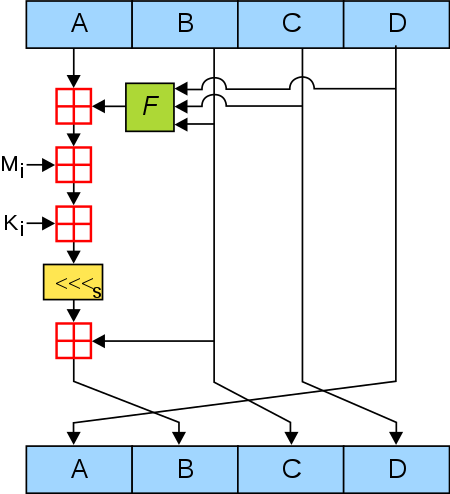
\includegraphics[scale=0.5]{imagenes/md5.png} 
	\caption{Esquema de los pasos seguidos en MD5 \cite{fotosmd5}.}
\end{figure}

\subsection{SHA-0}
SHA-0 es una función hash que apareció publicado en el Federal Information Processing Standard (FIPS-180) por el NIST en 1993 \cite{Penard2008}. Está basado en \emph{MD4} y \emph{MD5}. El algoritmo transforma un mensaje de cualquier tamaño hasta $2^{64}$ bits y los transforma en hashes de 160 bits.\\
El funcionamiento de SHA-0 es el siguiente \cite{sha0}:
\begin{enumerate}
	\item Al igual que en MD5, el mensaje se rellena con un único bit '1' seguido de 0-511 bits '0'. A continuación se añade una representación de 64 bits de la longitud del mensaje donde el número de ceros es elegido para asegurar que la longitud total del mensaje es un múltiplo de 512 bits. El mensaje se divide en bloques de 512 bits: $M_1,...,M_n$.
	\item Para la primera iteración se utiliza un buffer predefinido:
	$$
		h_0=(67452301_x, EFCDAB89_x, 98BADCFE_x, 10325476_x, C3D2E1F0_x).
	$$
	\item Cada bloque $M_j$ es pasado por la función de compresión junto con el valor actual de $h_{j-1}$, la salida es el nuevo valor de $h_j$, la operación se puede resumir en:
	$$
		h_j=compresión(M_j,h_{j-1}).
	$$
	\item $h_n$ es la salida de la función hash.
\end{enumerate}
Los pasos seguidos en la función de compresión son:
\begin{enumerate}
	\item Se divide el bloque $M_j$ de 512 bits en bloques 16 bloques de 32 bits $W_0,W_1,...,W_{15}$. 
	\item Se expanden los 16 bloques de 32 bits en 80 bloques a partir de la siguiente ecuación en recurrencias:
	$$
		W_i=W_{i-3}\oplus W_{i-8}\oplus W_{i-14}\oplus W_{i-16},\; i=16,...,79.
	$$
	Esta expansión se nota como exp(.).
	\item Divide $h_{j-1}$ en 5 registros \emph{A, B, C, D} y \emph{E} como:
	$$
		h_{j-1} = (A_0, B_0, C_0, D_0, E_0).
	$$
	\item Para $i=0,...,79$ hacemos:
	$$
		A_{i+1}=(A_i\lll5)+f_i(B_i,C_i,D_i)+E_i+K_i) \mod 2^{32},
	$$
	$$
		B_{i+1}=A_i,\: C_{i+1}=(B_i\lll30),\: D_{i+1}=C_i,\: E_{i+1}=D_i.
	$$
	Donde las funciones y las constantes están definidas en la tabla \ref{tablasha0}.
	\item La salida de la función sería:
	$$
		h_n=(A_0+A_{80}, B_0+B_{80}, C_0+C_{80}, D_0+D_{80}, E_0+E_{80}).
	$$
\end{enumerate}

\begin{table}[H]
	\begin{center}
		\begin{tabular}{| l | l | l |}
				\hline
				Rondas & $f_i(B,C,D)$ & $K_i$\\ \hline
				$0\leq i\leq 19$ & $BC\vee BD$ & $5AD9EBA1_x$\\ \hline
				$20\leq i\leq 39$ & $B\oplus C\oplus D$ & $6ED9EBA1_x$\\ \hline
				$40\leq i\leq 59$ & $BC\vee BD\vee CD$ & $8F1BBCDC_x$\\ \hline
				$60\leq i\leq 79$ & $B\oplus C\oplus D$ & $CA62C1D6_x$\\ \hline
		\end{tabular}
		\caption{Funciones y constantes usadas en la función de compresión de SHA-0 \cite{sha0}.}
	\label{tablasha0}
	\end{center}
\end{table}

\subsection{SHA-1}
La función SHA-1 es una función hash diseñada en 1995 por la \emph{National Security Agency} (NSA) dado que que se encontró varias colisiones y vulnerabilidades en la función SHA-0 \cite{Penard2008}.\\
Su funcionamiento es muy similar al de la función SHA-0 variando en las funciones y variables usadas en las distintas rondas de la función de compresión. En la tabla \ref{tablasha1} se pueden ver los nuevos valores utilizados.\\
\begin{table}[htb]
	\begin{center}
		\begin{tabular}{| l | l | l |}
				\hline
				Rondas & $f_i(B,C,D)$ & $K_i$\\ \hline
				$0\leq i\leq 19$ & $(B\wedge C)\oplus (\overline{B}\wedge D)$ & $5A827999_x$\\ \hline
				$20\leq i\leq 39$ & $B\oplus C\oplus D$ & $6ED6EBA1_x$\\ \hline
				$40\leq i\leq 59$ & $(B\wedge C)\oplus (B\wedge D) \oplus (C\wedge D)$ & $8FABBCDC_x$\\ \hline
				$60\leq i\leq 79$ & $B\oplus C\oplus D$ & $CA62C1D6_x$\\ \hline
		\end{tabular}
		\caption{Funciones y constantes usadas en la función de compresión de SHA-1 \cite{sha1}.}
		\label{tablasha1}
	\end{center}
\end{table}

En siguiente imagen se puede observar un esquema del proceso para obtener un el hash seguido por las funciones  SHA-0 y SHA-1 donde \textbf{F} será la función de compresión.
\begin{figure}[htb]
	\centering
	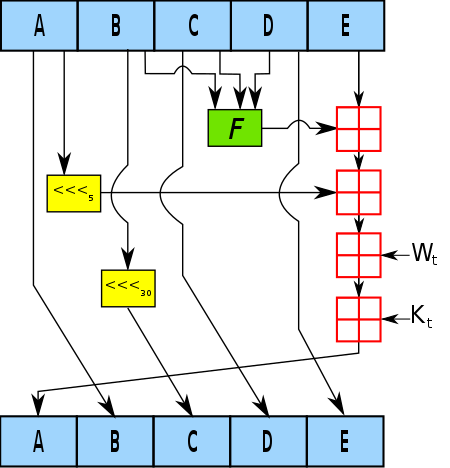
\includegraphics[scale=0.5]{imagenes/sha0-1.png} 
	\caption{Esquema de los pasos seguidos en SHA-0 y SHA-1 \cite{fotosha10}.}
\end{figure}

\subsection{SHA-256}
La función SHA-256 pertenece a la familia SHA-2 que es un conjunto de funciones hash diseñadas por la NSA en 2001 \cite{Penard2008}. Esta familia está compuesta por las funciones SHA-224, SHA-256, SHA-384 y SHA-512 donde el número del final indica el tamaño de bloque en el que se dividirá el mensaje. Nos centraremos en la función SHA-256 que como he comentado anteriormente es la que se utiliza en las aplicaciones de mensajería actualmente.\\
El funcionamiento de las función es el siguiente\cite{Function2016}:\\
\begin{enumerate}
	\item Al igual que en SHA-0 y SHA-1 se rellena el mensaje de la misma manera y se fragmenta en bloques de 512 bits: $M_1,...,M_n$.
	\item Para la primera iteración se utiliza un buffer predefinido:
	$$
		h_0=(H_1, H_2, H_3, H_4, H_5, H_6, H_7, H_8),
	$$
	donde:\\
	$H_1=6A09E776$\\
	$H_2=BB67AE85$\\
	$H_3=3C6EF372$\\
	$H_4=A54FF53A$\\
	$H_5=510E527F$\\
	$H_6=9B05688C$\\
	$H_7=1F83D9AB$\\
	$H_8=5BE0CD19$\\
	\item Cada bloque $M_j$ es pasado por la función de compresión junto con el valor actual de $h_{j-1}$, la salida es el nuevo valor de $h_j$, la operación se puede resumir en:
	$$
		h_j=compresión(M_j,h_{j-1}).
	$$
	\item $h_n$ es la salida de la función hash.
\end{enumerate}
Los pasos seguidos en la función de compresión son:
\begin{enumerate}
	\item Se divide el bloque $M_j$ de 512 bits en bloques 16 bloques de 32 bits $W_0,W_1,...,W_{15}$. 
	\item Se expanden los 16 bloques de 32 bits en 63 bloques a partir de la siguiente ecuación en recurrencias:
	$$
		W_i=\sigma_1(W_{j-2})+W_{j-7}+\sigma_0(W_{j-16}),\; i \in \{16...63\}.
	$$
	\item Divide $h_{j-1}$ en \emph{A, B, C, D, E, F, G} y \emph{H} como:
	$$
		h_{j-1} = (A_0, B_0, C_0, D_0, E_0, F_0, G_0, H_0).
	$$
	\item Para $i=0,...,63$ hacemos:
	$$
		A_{i+1}=H_i+\Sigma_1(E_i)+Ch(E_i,F_i,G_i)+K_j+W_j+\Sigma_0(A_i)+Maj(A_i,B_i,C_i),
	$$
	$$
		B_{i+1}=A_i,\: C_{i+1}=B_i,\: D_{i+1}=C_i,\: F_{i+1}=E_i\: G_{i+1}=F_i,\: H_{i+1}=G_i,
	$$
	$$
		E_{i+1}=D_i+H_i+\Sigma_1(E_i)+Ch(E_i,F_i,G_i)+K_j+W_j.
	$$
	Donde las funciones y las constantes están definidas en la tabla \ref{tablasha0}.
	\item La salida de la función sería:
	$$
		h_j=(A_0+A_{63}, B_0+B_{63}, C_0+C_{63}, D_0+D_{63}, E_0+E_{63}, F_0+F_{63}, G_0+G_{63}, H_0+H_{63}).
	$$
\end{enumerate}
Donde tenemos que:
$$
	Ch(x,y,z) = (x\wedge y)\oplus (\overline{x}\wedge z),
$$
$$
	Maj(x,y,z) = (x\wedge y)\oplus (x\wedge z)\oplus (y\wedge z),
$$
$$
	\Sigma_0(x) = (x\ggg2)\oplus (x\ggg13)\oplus (x\ggg22),
$$
$$
	\Sigma_1(x) = (x\ggg6)\oplus (x\ggg11)\oplus (x\ggg25),
$$
$$
	\sigma_0(x) = (x\ggg7)\oplus (x\ggg18)\oplus (x\lll3),
$$
$$
	\sigma_1(x) = (x\ggg17)\oplus (x\ggg19)\oplus (x\lll10).
$$

%\newpage
En la siguiente imagen podemos ver un esquema de los pasos seguidos en las funciones SHA-2.\\
\begin{figure}[htb]
	\centering
	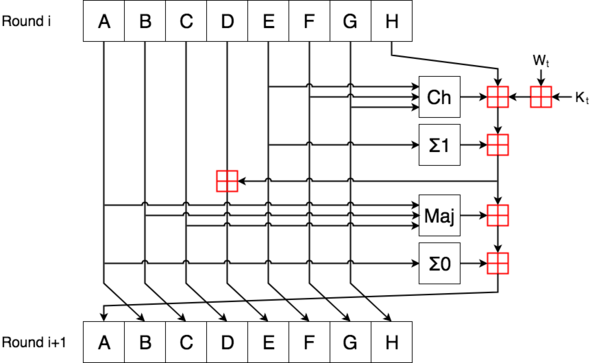
\includegraphics[scale=0.5]{imagenes/sha2.png} 
	\caption{Esquema de los pasos seguidos en las funciones de la familia SHA-2 \cite{sha2wikipedia}.}
\end{figure}

Con esto concluye el capítulo en el cual se han introducido todas las herramientas necesarias para entender los criptosistemas de las aplicaciones de mensajería. En el próximo capítulo procederé a explicar los criptosistemas utilizados en algunas de las aplicaciones de mensajería más populares.

%
\chapter{Aritmética modular y cuerpos finitos}
En este capítulo presentaré la teoría necesaria de aritmética modular y de cuerpos finitos para comprender adecuadamente las operaciones que se realizan en algoritmos como AES y RSA.

\section{Aritmética modular}
La aritmética modular es una de las piezas fundamentales de la criptografía y es especialmente importante en algoritmos como RSA. A continuación voy presentar unos resultados  que serán relevantes a la hora de explicar los distintos algoritmos utilizados.
\begin{definicion}
Se conoce a la función $\phi(n)$ como la función de Euler. Esta es definida como $\phi(n)=|\mathbb{Z}^*_n|$ y se puede calcular como $$\phi(n)=n\prod_{p_i|n}\left(1-\frac{1}{p_i}\right).$$
\end{definicion}
\begin{teorema}
	(Teorema de Euler) Sean a,n $\in \mathbb{Z}$ primos relativos entre sí, entonces $a^{\phi(n)}\equiv 1 \mod n$.
\end{teorema}\vspace*{-7mm}
\begin{proof}
		Sea $n\in \mathbb{Z^+}$ que verifica que $\operatorname{mcd}(a,n)=1$ y definimos $S$ como el conjunto de las unidades modulo $n$, $S=\{u_1,u_2,\dots,u_{\phi(n)}\}$ donde $1\leq u_i\leq n-1$, $\operatorname{mcd}(u_i,n)=1$ y $u_i\neq u_j$ $\forall i,j \in \{1,\dots,\phi(n)\}$ con $ i\neq j$.\\
	Multiplicando  los elementos de $S$ por $a$ obtenemos 
	$$
		aS=\{au_1,au_2,\dots,au_{\phi(n)}\}
	$$
	Como $\operatorname{mcd}(a,n)=1$ entonces $a\mod n$ es una unidad y por tanto $aS$ será el conjunto de las unidades módulo $n$. Y dado que los elementos de $S$ y los de $aS$ coinciden módulo $n$, el producto de estos será el mismo módulo $n$ por lo que obtenemos 
	$$
		u_1u_2\dots u_{\phi(n)} \equiv (au_1)(au_2)\dots (au_{\phi(n)})\mod n.
	$$
	Sacando como factor común $a$ tenemos 
	$$
		u_1u_2\dots u_{\phi(n)} \equiv a^{\phi(n)}u_1u_2\dots u_{\phi(n)}\mod n. 
	$$
\end{proof}\\

\begin{teorema}
		(Teorema pequeño de Fermat) Sea $a \in \mathbb{Z}$ y $p$ un número primo tal que $\operatorname{mcd}(a,p)=1$. Entonces
	$$
		a^{p-1} \equiv 1 \mod p.
	$$
\end{teorema}\vspace*{-7mm}
\begin{proof}
		Sea $a \in \mathbb{Z}$. Tomamos los $p-1$ primeros múltiplos positivos de $a$ que serán de la forma $a, 2a,\dots,(p-1)a$. El resto resultante de dividir los $p-1$ múltiplos positivos de $a$ por $p$ corresponden a 1,2,3,$\dots,p-1$.\\
	Multiplicando ahora todas las congruencias obtenemos 
	$$
		a^{p-1}·(p-1)! \equiv (p-1)! \mod p.
	$$
	Como tenemos que $p\nmid (p-1)!$ se cumple que $\operatorname{mcd}(p,p-1)=1$ y por tanto cancelando en la expresión anterior obtenemos
	$$
		a^{p-1} \equiv 1 \mod p. 
	$$
\end{proof}

Cabe a destacar que el Teorema de Fermat es un caso particular del Teorema de Euler.\\

\begin{teorema}
		(Teorema Chino del Resto) Sean $a_1, a_2\in \mathbb{Z}$ y $p,q \in \mathbb{N}$ tales que $\operatorname{mcd}(p,q) = 1$. Entonces el sistema
		$$
			x\equiv a_1 \mod p,
		$$\vspace*{-11mm}

		$$
			x\equiv a_2 \mod q,
		$$
	tiene solución única módulo $n=pq$. Además, la solución está dada por
	$$
		x\equiv a_1\cdot q\cdot d_1 +a_2\cdot p\cdot d_2 \mod n,
	$$
	donde se cumple
	$$
		q\cdot d_1 \equiv 1 \mod p,
	$$
	$$
		p\cdot d_2 \equiv 1 \mod q.
	$$
\end{teorema}
\begin{proof}
		Veamos la existencia de la solución. Sea $N=p\cdot q$. Como por hipótesis tenemos que $\operatorname{mcm}(p,q)=1$, por Bézout existen enteros $d_i$, $s_i$ con $i=1,2$ tales que $d_1p+s_1q=1$ y $d_2q+s_2p=1$. Tomando módulo $p$ y $q$ tenemos que 
	$$
		d_1\cdot p \equiv 1 \mod q,
	$$
	$$
		d_2\cdot q \equiv 1 \mod p.
	$$
	Definiendo 
	$$
		x :=  a_1\cdot q\cdot d_1 +a_2\cdot p\cdot d_2,
	$$
	se consigue que $x$ sea la solución del sistema. Además, trabajando módulo $p$ y $q$ obtenemos que $x\equiv a_1 \mod p$ y $x\equiv a_2 \mod q$.\\
	Una vez vista la existencia de la solución quedaría demostrar la unicidad. Para ello supongamos que existen dos números enteros distintos $x$ e $y$ tales que 
		\begin{equation}
			\begin{split}
				x \equiv a_1 \mod p,\notag\\
				y \equiv a_1 \mod p.\notag
			\end{split}
		\end{equation}
	Y también 
		\begin{equation}
			\begin{split}
				x \equiv a_2 \mod q,\notag\\
				y \equiv a_2 \mod q.\notag
			\end{split}
		\end{equation}
	Esto implica que $x-y\equiv0 \mod p$ y $x-y\equiv0 \mod q$. Como $p$ y $q$ son coprimos, tenemos que $x-y\equiv 0 \mod N$, luego se da que $x\equiv y \mod N$ llegando así a una contradicción. \qedhere
\end{proof}

\begin{proposicion}
	Sea $n = pq$, donde p y q son dos primos distintos. Si $x\equiv 1 \mod \phi(n)$, entonces $a^x\equiv a\mod n$ para todo $ a \n \in \mathbb{Z}$.
\end{proposicion}\vspace*{-5mm}

	\begin{proof}
		Si $a$ es múltiplo de $n$, entonces se cumple que $a^x \equiv 0 \equiv a \mod n$. Si $a$ y $n$ son coprimos, $\operatorname{mcm}(a,n) = 1$. Entonces tendríamos que $a^x \equiv a \mod n$ por el Teorema de Euler.\\
		Nos quedaría ver ocurre en el caso de $a$ sea múltiplo de $p$ o de $q$, pero no de ambos. Por simetría supondremos que a es múltiplo de $p$, pero no de $q$. En este caso tenemos que $a^x \equiv 0 \equiv a \mod p$  y $a^x \equiv a \mod q$ por el Teorema de Fermat. Como $p$ y $q$ son coprimos entre sí, aplicando el Teorema Chino del Resto se deduce que $a^x \equiv a \mod n$.\qedhere
	\end{proof}

\section{El cuerpo de Galois $\operatorname{GF}(2^n)$}
Tanto para explicar el funcionamiento de las rondas de AES como para desarrollar la teoría de Curvas Elípticas en $\operatorname{GF}(2^n)$ es necesario introducir el cuerpo $\operatorname{GF}(2^n)$, el cual debido a las propiedades que tiene es muy utilizado en criptografía.\\
Sea $\mathbb{Z}_2[x]$ el conjunto de polinomios con coeficientes en $\mathbb{Z}_2$, es decir, el conjunto de polinomios cuyos coeficientes solo valen 0 ó 1. Así los polinomios pueden ser representados por una cadena de bits.
 Un ejemplo sería el polinomio $f(x)=x^4+x^3+x+1$ que quedaría representado como 11011. 
Además si lo sumamos con otro polinomio como puede ser $g(x)=x^2+x+1$, tenemos que $f(x)+g(x)=x^4+x^3+x^2$, que equivale a hacer la operación XOR entre 11011 y 00111, por lo que a nivel computacional, es muy fácil implementar estas operaciones.\\
Podemos definir el cuerpo $\operatorname{GF}(2^n)$ como $\mathbb{Z}_2[x]/(a(x))$, con $a(x)$ un polinomio irreducible en $\mathbb{Z}/(a(x))$. Tenemos que la existencia del inverso de cualquier polinomio no nulo está asegurada por el algoritmo Extendido de Euclídes.\\ 
Principalmente se trabaja con $\operatorname{GF}(2^n)$ debido a que la implementación de las operaciones de este es más sencilla que la implementación en las que se utilizan otros cuerpos. Esta sencillez de implementación se traduce en unos algoritmos con tiempos de ejecución menores a pesar de tener el mismo orden de complejidad.\\
A continuación presentaré el cuerpo $\operatorname{GF}(2^8)$, ya que será necesario para entender adecuadamente las operaciones utilizadas en AES. La información ha sido obtenida de \cite{criptografia} y \cite{dem1}.\\
Tenemos que $\operatorname{GF}(2^8)=\mathbb{F}_{256}$ por lo que por comodidad trabajaremos con este último.\\
Por definición tenemos que para $p$ número primo y $n$ un entero primitivo se define el cuerpo $\mathbb{F}_{p^n}$ al único cuerpo existente con $p^n$ elementos. En particular para trabajar con $\mathbb{F}_{256}$ tomamos $p=2$ y $n=8$.\\
Para construir $\mathbb{F}_{256}$ necesitamos un polinomio de grado 8, con coeficientes en $\mathbb{Z}_2$ y que sea irreducible. En total hay 30 polinomios con esas características donde algunos de ellos son 
$x^8+x^4+x^3+x+1$, $\:x^8+x^4+x^3+x^2+1$, $x^8+x^5+x^3+x+1$, $x^8+x^5+x^3+x^2+1$, $x^8+x^5+x^4+x^3+1$, $x^8+x^5+x^4+x^3+x^2+x+1$ y $x^8+x^6+x^3+x^2+1$.\\ 
Cabe a destacar que cualquiera de los polinomios serviría para definir $\mathbb{F}_{256}$ y además no habría ninguna diferencia en la seguridad en los criptosistemas que lo utilicen. 
Para AES se tomó el polinomio $x^8+x^4+x^3+x+1$, por lo que a partir de ahora trabajaremos con $\mathbb{Z}_2[x]_{a(x)}$ siendo $a(x)$ el polinomio $x^8+x^4+x^3+x+1$.\\
Los elementos que conformarán este cuerpo serán clases de equivalencia de polinomios  de grado menor que 8. Cada elemento podrá ser representado de tres formas distintas además de la forma polinomial, como número binario, número hexadecimal y número decimal. Por ejemplo el polinomio $x^5+x+1$ quedaría representado como $00100011$ de manera decimal, $23$ en hexadecimal y $35$ en decimal.\\
Al ser $\mathbb{F}_{256}$ un cuerpo tenemos que tiene dos operaciones, la operación suma que representaremos como $+$ y la operación producto que representaremos como $\cdot$.\\
La operación $+$ equivale a la suma en $\mathbb{Z}_2$ y usando la notación en binario, tendríamos que equivaldría con la operación XOR como ya he mencionado anteriormente. El opuesto para la suma de un elemento equivalente a sí mismo por lo que no habría diferencia entre sumar por un número o por su apuesto, luego tendríamos que la suma es la misma operación que la resta.\\
La operación $\cdot$  es mucho más compleja ya que en principio habría que realizar la operación en notación polinomial y luego calcular el resto de dividir por $x^8+x^4+x^3+x+1$. Para calcular el inverso tendríamos que utilizar el algoritmo extendido de Euclídes. Ambos algoritmos tienen una complejidad algorítmica importante, pero se puede reducir. A continuación recordaré unos resultados de cuerpos finitos que nos permitirán obtener unos métodos que reducirán mucho esa complejidad.\\
\begin{definicion}
	Sea $K=\mathbb{F}_q$ un cuerpo finito $(q=p^n)$. Un elemento primitivo de $K$ es un elemento $\alpha$ que tiene $q-1$ potencias distintas.
\end{definicion}

\begin{proposicion}
	Sea \mathbb{F} un cuerpo finito con $p^d$ elementos, donde $p$ es primo y $d\geq 1$, y sea
	$$
		x^{p^d}-x=m_1(x)m_2(x)\dots m_n(x)
	$$
	la factorización  de $x^{p^d}$ en polinomios irreducibles en $\mathbb{Z}_p[x]$. Entonces:
	\begin{enumerate}
		\item El polinomio mínimo de cada elemento de $\mathbb{F}$ es uno de los polinomios $m_1(x),\dots,m_n(x)$.
		\item Para cada $i$, el número de elementos de $\mathbb{F}$ con polinomio mínimo $m_i(x)$ es igal al grado de $m_i(x)$.
	\end{enumerate}
\end{proposicion}
\begin{proof}
		Como cada elemento de $\mathbb{F}$ es una de las raíces de $x^{p^d}-x$, entonces cada $m_i(x)$ tiene que tener un número de raíces en $\mathbb{F}$ equivalente a su grado. Como $m_i(x)$ es irreducible, entonces tienen que haber un polinomio mínimo para cada una de esas raíces.
\end{proof}

\begin{teorema}
	El orden de todo elemento $\alpha \in \mathbb{F}^*_q$ divide a $q-1$. 
\end{teorema}
\begin{proof}
		Veamos que $\alpha^{q-1}=1$. Para ello tomamos el producto de todos los elementos no nulos de $\mathbb{F}_q$ y multiplicando cada miembro por $\alpha$ tenemos que \[ \prod_{\beta_i \in \mathbb{F}^*_q}\alpha\beta_i=\alpha^{q-1}\prod_{\beta_i \in \mathbb{F}^*_q}\beta_i\]
		ya que hay $q-1$ elementos en $\mathbb{F}^*_q$ y por tanto $\alpha^{q-1}=1$.\\
		A continuación llamamos $d$ al orden de $\alpha$ y suponemos que no divide a $q-1$, entonces tenemos que existe $r\in\mathbb{N}$ tal que $q-1=cd+r$ y por tanto se cumple que $\alpha^r=\alpha^{q-1-cd}=1$ llegando a una contradicción con la minimalidad del orden de $d$.
\end{proof}

\begin{teorema}
	Todo cuerpo finito tiene un generador. Si $g$ es un generador de $\mathbb{F}^{*}_q$, entonces $g^j$ es también un generador si y sólo si $\operatorname{gcd}(j,q-1)=1$. En particular, hay $\phi(q-1)$ generadores distintos de $\mathbb{F}^*_q$.
\end{teorema}
\begin{proof}
		Supongamos $\alpha \in \mathbb{F}^*_q$ con orden $n$. Veamos primero $\alpha^j$ tiene orden $d$ si y solamente si $\operatorname{gcd}(j,d)=1$.\\
		Para ver que es condición necesaria tomamos un $j$ que verifique $\operatorname{gcd}(j, d)=d'$ con $d'$\textgreater$ 1$, tenemos que $a=\frac{d}{d'}$ y $b=\frac{j}{d'}$ son números enteros y además se cumple que $(\alpha^j)^a=(\alpha^d)^b=1$. Luego se cumple que el orden de $\alpha^j$ es $a$\textless $d$.\\
		Veamos que también es condición suficiente.\\ Para ello tomamos un $j$ que verifique $\operatorname{gcd}(j,d)=1$ y supongamos que $\alpha^j$ tiene orden $k$\textless $d$. Como se cumple que $1=(\alpha^j)^k=(a^k)^j$ y $d$ es el orden de $\alpha$ tenemos que $(\alpha^k)^d=(a^d)^k=1^k=1$.\\
		Por tanto, se cumple que  $(\alpha^k)^1=(\alpha^k)^{\operatorname{gcd}(j,d)}=(\alpha^k)^{uj}(\alpha^k)^{vd}=1$. Llegando así a una contradicción, ya que hemos supuesto que $\alpha$ no tiene orden $d$.\\
		Luego tenemos que el orden de $\alpha^j$ es $d$.\\
		Como las potencias de $\alpha,(\alpha,\alpha^2,\dots,\alpha^d=1)$ cumplen la ecuación $X^d=1$ y son raíces de las misma, se cumple que no hay más elementos con orden $d$. Luego $\mathbb{F}^*_q$ tiene $\phi(d)$ elementos distintos de orden $d$.\\
		Por último vamos a ver la existencia de un generador $g$ de $\mathbb{F}_q^*$.\\
		Sabemos que la función \emph{phi de Euler} cumple en $q-1$ que $\sum_{d|q-1}\phi(d)=q-1$ y como se cumple que todo elemento de $\mathbb{F}^*_q$ tiene un orden $d$ divisor de $q-1$, necesariamente existen elementos de $\mathbb{F}^*_q$ con orden $d$ para todo $d|q-1$ y en particular se cumple la hipótesis del enunciado.
\end{proof}

\begin{corolario}
		El grupo multiplicativo de todos los elementos no nulos de un cuerpo finito es cíclico.
\end{corolario}

Si $\alpha$ es un elemento primitivo de $\mathbb{F}_q$, los $q-1$ elementos de la forma\\
$$
	\alpha^0=1,\;\; \alpha^1=\alpha,\;\dots\; ,\alpha^{q-2}
$$
serán todos distintos y no nulos. Por tanto serán todos los elementos no nulos de $\mathbb{F}_q$. Además, se verifica que $\alpha^{q-1}=\alpha^0$ por lo que para cualquier $n \in \mathbb{Z}$ se cumple que $\alpha^n=\alpha^{n\mod q-1}$.\\
%\begin{teorema}
	%Todo cuerpo finito tiene al menos un elemento primitivo.
%\end{teorema}
Salvo para $q=2$, el número de elementos primitivos de $\mathbb{F}_q$ es $\phi(q-1)$. Para el caso $q=13$ se tiene que $\phi(12)=\phi(2^2\cdot 3)=2\cdot2=4$, luego $\mathbb{Z}_{13}$ tiene 4 elementos primitivos que son 2, 6, 7 y 11. En $\mathbb{F}_{256}$ tenemos que hay $\phi(256)=128$ elementos primitivos.

Ahora para multiplicar dos elementos pertenecientes a $\mathbb{Z}_{13}$ podemos usar su logaritmo en base 2, el exponente que hay que elevar 2 para obtener el número, sumar los logaritmos y reducirlos base 13 y elevar 2 al resultado. Un ejemplo sería:
$$
	10\cdot12=2^{10}\cdot2^{6}=2^{16}=2^3=8.
$$
Para calcular el inverso sería:
$$
	12^{-1}=(2^6)^{-1}=2^{12-6}=2^6=12.
$$
Esta es la idea que nos permite optimizar las multiplicaciones y los cálculos de inversos en $\mathbb{F}_{256}$. Para ello elegimos un elemento primitivo que nos servirá de generador, en este caso nosotros utilizaremos el más pequeño, que es $[x+1]$ en notación polinomial, 00000011 en binario, 03 en hexadecimal y 3 en binario. Por comodidad trabajaremos en hexadecimal. 

\begin{table}[!htb]
    %\begin{adjustwidth}{-.8in}{-.8in}  
\resizebox{\textwidth}{!}{%
\begin{tabular}{|l|l|l|l|l|l|l|l|l|l|l|l|l|l|l|l|l|}
\hline
\multicolumn{1}{|r|}{} & 0  & 1  & 2  & 3  & 4  & 5  & 6  & 7  & 8  & 9  & A  & B  & C  & D  & E  & F  \\ \hline
0                      & 01 & 03 & 05 & 0F & 11 & 33 & 55 & FF & 1A & 2E & 72 & 96 & A1 & F8 & 13 & 35 \\ \hline
1                      & 5F & E1 & 38 & 48 & D8 & 73 & 95 & A4 & F7 & 02 & 06 & 0A & 1E & 22 & 66 & AA \\ \hline
2                      & E5 & 34 & 5C & E4 & 37 & 59 & EB & 26 & 6A & BE & D9 & 70 & 90 & AB & E6 & 31 \\ \hline
3                      & 53 & F5 & 04 & 0C & 14 & 3C & 44 & CC & 4F & D1 & 68 & B8 & D3 & 6E & B2 & CD \\ \hline
4                      & 4C & D4 & 67 & A9 & E0 & 3B & 4D & D7 & 62 & A6 & F1 & 08 & 18 & 28 & 78 & 88 \\ \hline
5                      & 83 & 9E & B9 & D0 & 6B & BD & DC & 7F & 81 & 98 & B3 & CE & 49 & DB & 76 & 9A \\ \hline
6                      & B5 & C4 & 57 & F9 & 10 & 30 & 50 & F0 & 0B & 1D & 27 & 69 & BB & D6 & 61 & A3 \\ \hline
7                      & FE & 19 & 2B & 7D & 87 & 92 & AD & EC & 2F & 71 & 93 & AE & E9 & 20 & 60 & A0 \\ \hline
8                      & FB & 16 & 3A & 4E & D2 & 6D & B7 & C2 & 5D & E7 & 32 & 56 & FA & 15 & 3F & 41 \\ \hline
9                      & C3 & 5E & E2 & 3D & 47 & C9 & 40 & C0 & 5B & ED & 2C & 74 & 9C & BF & DA & 75 \\ \hline
A                      & 9F & BA & D5 & 64 & AC & EF & 2A & 7E & 82 & 9D & BC & DF & 7A & 8E & 89 & 80 \\ \hline
B                      & 9B & B6 & C1 & 58 & E8 & 23 & 65 & AF & EA & 25 & 6F & B1 & C8 & 43 & C5 & 54 \\ \hline
C                      & FC & 1F & 21 & 63 & A5 & F4 & 07 & 09 & 1B & 2D & 77 & 99 & B0 & CB & 46 & CA \\ \hline
D                      & 45 & CF & 4A & DE & 79 & 8B & 86 & 91 & A8 & E3 & 3E & 42 & C6 & 51 & F3 & 0E \\ \hline
E                      & 12 & 36 & 5A & EE & 29 & 7B & 8D & 8C & 8F & 8A & 85 & 94 & A7 & F2 & 0D & 17 \\ \hline
F                      & 39 & 4B & DD & 7C & 84 & 97 & A2 & FD & 1C & 24 & 6C & B4 & C7 & 52 & F6 & 01 \\ \hline
\end{tabular}}
	\label{antilogaritmos}
	%\end{adjustwidth}
\caption{Tabla de los antilogaritmos de $[x+1]$}
\end{table}
Por ejemplo para calcular el resultado de $[x+1]^{125}=(03)^{125}$ lo que hacemos es escribir 125 en hexadecimal que es 7D. A continuación miramos en la tabla, la fila 7 y la columna D que nos da 20 luego tendríamos que $(03)^{125}=20$. Pasándolo a forma polinomial tenemos que $[x+1]^{125}=x^5$.\\
Para construir la tabla es mejor usar la forma binaria.\\

A continuación vamos a construir la tabla inversa de la anterior, esta nos permitirá calcular dado un $z \in \mathbb{F}_{256}$ con $z \neq 0$ el valor de $y$ que verifica $[x+1]^y=z$ que denominaremos $\log_{x+1}(z)$.
\begin{table}[!htb]
    %\begin{adjustwidth}{-.8in}{-.8in}  
\resizebox{\textwidth}{!}{%
\begin{tabular}{|l|l|l|l|l|l|l|l|l|l|l|l|l|l|l|l|l|}
\hline
  & 0  & 1  & 2  & 3  & 4  & 5  & 6  & 7  & 8  & 9  & A  & B  & C  & D  & E  & F  \\ \hline
0 &    & 00 & 19 & 01 & 32 & 02 & 1A & C6 & 4B & C7 & 1B & 68 & 33 & EE & DF & 03 \\ \hline
1 & 64 & 04 & E0 & 0E & 34 & 8D & 81 & EF & 4C & 71 & 08 & C8 & F8 & 69 & 1C & C1 \\ \hline
2 & 7D & C2 & 1D & B5 & F9 & B9 & 27 & 6A & 4D & E4 & A6 & 72 & 9A & C9 & 09 & 78 \\ \hline
3 & 65 & 2F & 8A & 05 & 21 & 0F & E1 & 24 & 12 & F0 & 82 & 45 & 35 & 93 & DA & 6E \\ \hline
4 & 96 & 8F & DB & BD & 36 & D0 & CE & 94 & 13 & 5C & D2 & F1 & 40 & 46 & 83 & 38 \\ \hline
5 & 66 & DD & FD & 30 & BF & 06 & 8B & 62 & B3 & 25 & E2 & 98 & 22 & 88 & 91 & 10 \\ \hline
6 & 7E & 6E & 48 & C3 & A3 & B6 & 1E & 42 & 3A & 6B & 28 & 54 & FA & 85 & 3D & BA \\ \hline
7 & 2B & 79 & 0A & 15 & 9B & 9F & 5E & CA & 4E & D4 & AC & E5 & F3 & 73 & A7 & 57 \\ \hline
8 & AF & 58 & A8 & 50 & F4 & EA & D6 & 74 & 4F & AE & E9 & D5 & E7 & E6 & AD & E8 \\ \hline
9 & 2C & D7 & 75 & 7A & EB & 16 & 0B & F5 & 59 & CB & 5F & B0 & 9C & A9 & 51 & A0 \\ \hline
A & 7F & 0C & F6 & 6F & 17 & 74 & 49 & EC & D8 & 43 & 1F & 2D & A4 & 76 & 7B & B7 \\ \hline
B & CC & BB & 3E & 5A & FB & 60 & B1 & 86 & 3B & 52 & A1 & BC & AA & 55 & 29 & 9D \\ \hline
C & 97 & B2 & 87 & 90 & 61 & BE & DC & FC & B5 & 95 & CF & CD & 37 & 3F & 5B & D1 \\ \hline
D & 53 & 39 & 84 & 3C & 41 & A2 & 6D & 47 & 14 & 2A & 9E & 5D & 56 & F2 & D3 & AB \\ \hline
E & 44 & 11 & 92 & D9 & 23 & 20 & 2D & 89 & B4 & 7C & B8 & 26 & 77 & 99 & E3 & A5 \\ \hline
F & 67 & 48 & ED & DE & C5 & 31 & FE & 18 & 0D & 63 & 8C & 80 & C0 & F7 & 70 & 07 \\ \hline
\end{tabular}}
	\label{potenciasinversas}
    %\end{adjustwidth}
\caption{Tabla de los logaritmos de $[x+1]$}
\end{table}

A partir de estas dos tablas ya podemos hacer sin mucha dificultad a nivel computacional multiplicaciones y cálculo de inversos. En general para realizar el producto de dos elementos $X$ e $Y$ lo haremos de la siguiente manera:
$$
	X\cdot Y = A\log((\log_{x+1}(X)+log_{x+1}(Y)) \mod 255).
$$
Donde $A\log$ es el antilogaritmo.\\
Análogamente para calcular el inverso tenemos:
$$
	X^{-1} = A\log(FF-\log_{x+1}(X)).
$$

Por ejemplo para calcular $[x^7+x^6+x^4+x^2+x]\cdot[x^6+x^5+x^4+x^2+1]$ hacemos lo siguiente:
\begin{enumerate}
	\item Pasamos ambos polinomios a la forma hexadecimal como hemos visto anteriormente, en este caso nos quedaría $D6$ y $75$.
	\item Nos vamos a la tabla de logaritmos y obtenemos que $\log_{03}(D6)=6D$ y $\log_{03}(75)=9F$.
	\item Sumamos ambos resultados y lo reducimos módulo $255$, parar ello lo pasamos a decimal por comodidad $(109+159)\mod255=13$.
	\item Calculamos el antilogaritmo de $13=0D$ con la tabla y tenemos que vale $F8$ por lo que tenemos que $D6\cdot 75 = F8$.
\end{enumerate}

Con esto visto ya tendríamos todas las herramientas necesarias para poder describir con mayor profundidad el funcionamiento de los distintos criptosistemas que se utilizan en las aplicaciones de mensajería.


%
\chapter{Criptografía Simétrica. AES}
\label{chap:cuatro}

En este capítulo voy a explicar el cifrado Rijndael AES el cual es un cifrado de bloque simétrico muy utilizado actualmente por aplicaciones como \emph{Telegram}, \emph{WhatsApp} y \emph{FacebookChat} entre otras. Este algoritmo se usa principalmente para cifrar los mensajes ya que es muy eficiente a nivel computacional.\\
\section{El algoritmo Rijndael AES}
El algoritmo Rijndael llamado así en honor a sus dos autores Joan Daemen y Vicent Rijmen, es un algoritmo de cifrado por bloques que fue adoptado en octubre de 2000 por el NIST (\emph{National Institute for Standards and Technology}) para su empleo en aplicaciones criptográficas no militares en sustitución del algoritmo \emph{DES} después de un proceso de más tres años en los que se buscaba un algoritmo que fuera potente, eficiente y fácil de implementar.\\
Está diseñado para manejar longitudes de clave y de bloque variables entre los 128 y los 256 bits y aunque estos sean variables, en el estándar adoptado por el Gobierno de Estados Unidos en 2001 \cite{aesUsa} establece una longitud fija de bloque de 128 bits y una longitud de clave a escoger entre 128, 192 y 256 bits.\\
La información para los siguientes apartados de AES la he obtenido de \cite{En2011} y de \cite{criptografia}.
\newpage
\section{Estructura de AES}
AES es un algoritmo que se basa en aplicar un número determinado de rondas a un valor intermedio denominado \emph{estado} que puede ser representado por una matriz rectangular que posee cuatro filas y $N_{b}$ columnas. Análogamente, la clave tiene la misma estructura, una matriz de cuatro filas y $N_{k}$ columnas.
El bloque a cifrar o descifrar se traslada directamente byte a byte sobre la matriz de estado de columna en columna ($a_{0,0}, a_{1,0}, a_{2,0}, a_{3,0}, a_{0,1} \dots$).

\begin{table}[htb]
	\begin{center}
		\begin{tabular}{| c | c | c | c |}
				\hline
				$\math{a}_{0,0}$ & $\math{a}_{0,1}$ & $\math{a}_{0,2}$ & $\math{a}_{0,3}$\\ \hline
				$\math{a}_{1,0}$ & $\math{a}_{1,1}$ & $\math{a}_{1,2}$ & $\math{a}_{1,3}$\\ \hline
				$\math{a}_{2,0}$ & $\math{a}_{2,1}$ & $\math{a}_{2,2}$ & $\math{a}_{2,3}$\\ \hline
				$\math{a}_{3,0}$ & $\math{a}_{3,1}$ & $\math{a}_{3,2}$ & $\math{a}_{3,3}$\\ \hline
		\end{tabular}
		\caption{Ejemplo de matriz de estado con $N_b=4$(128 bits).}
	\end{center}
\end{table}

\begin{table}[htb]
	\begin{center}
		\begin{tabular}{| c | c | c | c |}
				\hline
				$\math{k}_{0,0}$ & $\math{k}_{0,1}$ & $\math{k}_{0,2}$ & $\math{k}_{0,3}$\\ \hline
				$\math{k}_{1,0}$ & $\math{k}_{1,1}$ & $\math{k}_{1,2}$ & $\math{k}_{1,3}$\\ \hline
				$\math{k}_{2,0}$ & $\math{k}_{2,1}$ & $\math{k}_{2,2}$ & $\math{k}_{2,3}$\\ \hline
				$\math{k}_{3,0}$ & $\math{k}_{3,1}$ & $\math{k}_{3,2}$ & $\math{k}_{3,3}$\\ \hline
		\end{tabular}
		\caption{Ejemplo de clave con $N_k=4$(128 bits).}
	\end{center}
\end{table}

En otros casos el bloque y la clave pueden ser representados como vectores de registro de 32 bits, donde cada registro esta compuesto por los bytes de la columna correspondiente ordenados en orden descendiente.\\

Siendo $B$ el bloque que queremos cifrar y $S$ la matriz de estado, el algoritmo AES con $n$ rondas se resume en:

\begin{enumerate}
	\item Calcular $K_0, K_1,...,K_n$ subclaves a partir de la clave $K$.
	\item $S\leftarrow B \oplus K_0$.
	\item Para $i=1$ hasta $n$ hacer:
	\begin{description}
			\item Aplicar la ronda \emph{i}-ésima del algoritmo con la subclave $K_i$.
	\end{description}
\end{enumerate}
Como las funciones usadas en cada ronda son invertibles, para descifrar aplicaremos las funciones inversas de las funciones usadas para cifrar en el orden opuesto.

\begin{table}[htb]
	\begin{center}
		\begin{tabular}{| c | c | c | c |}
				\hline
				& $N_b = 4$(128 bits) & $N_b = 6$(192 bits)& $N_b = 8$(256 bits)\\ \hline
				$N_k = 4$(128 bits)& 10 & 12 & 14\\ \hline
				$N_k = 6$(128 bits)& 12 & 12 & 14\\ \hline
				$N_k = 8$(128 bits)& 14 & 14 & 14\\ \hline
		\end{tabular}
		\caption{Número de rondas en función del tamaño de la clave y bloque.}
		\label{rondas_aes}
	\end{center}
\end{table}

En el algoritmo AES se define cada ronda como una composición de cuatro funciones invertibles diferentes, formando tres \emph{capas}. Estas funciones tienen un propósito específico.
\begin{itemize}
	\item \textbf{Capa de mezcla lineal:} formada por las funciones \emph{DesplazarFila} y \emph{MezclarColumnas} que permite obtener un alto nivel de difusión a lo largo de varias rondas.
	\item \textbf{Capa no lineal:} formada por la función \emph{ByteSub} y es la aplicación paralela de s-cajas con propiedades óptimas de no linealidad.
	\item \textbf{Capa de adición de clave:} es un simple \emph{o-exclusivo} entre el estado intermedio y la subclave correspondiente a cada ronda.
\end{itemize}

%\newpage
\section{Las Rondas de AES}
Una vez visto algunas de las propiedades de los cuerpos finitos, ya disponemos de las herramientas necesarias para describir las rondas de AES.
Dado que este algoritmo puede aplicarse para longitudes diferentes de bloque y clave, el número de rondas es variable, como se ha visto en \ref{rondas_aes}.\\
Siendo $S$ la matriz de estado y $K_i$ la subclave correspondiente a la ronda $i$-ésima, cada ronda posee esta estructura:
\begin{enumerate}
	\item $S \leftarrow ByteSub(S)$,
	\item $S \leftarrow DesplazarFila(S)$,
	\item $S \leftarrow MezclarColumnas(S)$,
	\item $S \leftarrow K_i \oplus S$.
\end{enumerate}
En la última ronda se hacen solo los tres primeros pasos del algoritmo.

	\subsubsection{ByteSub}
		La función \emph{ByteSub} es una sustitución no lineal que se aplica a cada byte de la matriz de estado mediante una s-caja 8\texttimes8. Se obtiene componiendo dos transformaciones:
		\begin{enumerate}
			\item Cada byte se considera como un elemento del $\operatorname{GF}(2^8)$ generado por el polinomio irreducible $m(x)=x^8+x^4+x^3+x+1$ y es sustituido por su inversa multiplicativa quedando el valor cero inalterado. 
			\item A continuación se aplica la siguiente transformación afín en $\operatorname{GF}(2^8)$ siendo $x_0, x_1,...,x_7$ los bits del byte correspondiente e $y_0, y_1,...,y_7$ los del resultado:

				\begin{equation*} 
					\begin{bmatrix} 
						y_0\\
						y_1\\
						y_2\\
						y_3\\
						y_4\\
						y_5\\
						y_6\\
						y_7\\
					\end{bmatrix}
					=
					\begin{bmatrix} % O matrices como esta de 4 x 3
						1 & 0 & 0 & 0 & 1 & 1 & 1 & 1\\
						1 & 1 & 0 & 0 & 0 & 1 & 1 & 1\\
						1 & 1 & 1 & 0 & 0 & 0 & 1 & 1\\
						1 & 1 & 1 & 1 & 0 & 0 & 0 & 1\\
						1 & 1 & 1 & 1 & 1 & 0 & 0 & 0\\
						0 & 1 & 1 & 1 & 1 & 1 & 0 & 0\\
						0 & 0 & 1 & 1 & 1 & 1 & 1 & 0\\
						0 & 0 & 0 & 1 & 1 & 1 & 1 & 1\\
					\end{bmatrix}
					\begin{bmatrix}
						x_0\\
						x_1\\
						x_2\\
						x_3\\
						x_4\\
						x_5\\
						x_6\\
						x_7\\
					\end{bmatrix}
					+
					\begin{bmatrix}
						1\\
						1\\
						0\\
						0\\
						0\\
						1\\
						1\\
						0\\
					\end{bmatrix}
			\end{equation*}
		\end{enumerate}
		La función inversa de $ByteSub$ es la aplicación inversa de la s-caja de cada byte de la matriz de estado.

	\subsubsection{DesplazarFila}
		Esta función desplaza a la izquierda de manera cíclica las filas de la matriz de estado. Cada fila $f_i$ se desplaza un número de posiciones $c_i$ diferente. Mientras que $c_0$ siempre es igual a cero, el resto de valores vine en función de $N_b$ como se puede ver en \ref{ciennb}.\\
		La función inversa será el desplazamiento de las filas de la matriz el mismo número de posiciones pero en el sentido contrario.

		\begin{table}[htb]
			\begin{center}
				\begin{tabular}{| c | c | c | c |}
						\hline
						$N_b$ & $c_1$ & $c_2$ & $c_3$\\ \hline
						4 & 1 & 2 & 3\\ \hline 
						6 & 1 & 2 & 3\\ \hline 
						8 & 1 & 3 & 4\\ \hline 
				\end{tabular}
				\caption{Valores de $c_i$ según el tamaño de bloque $N_b$}
				\label{ciennb}
			\end{center}
		\end{table}

		\begin{figure}[htb]
			\centering
			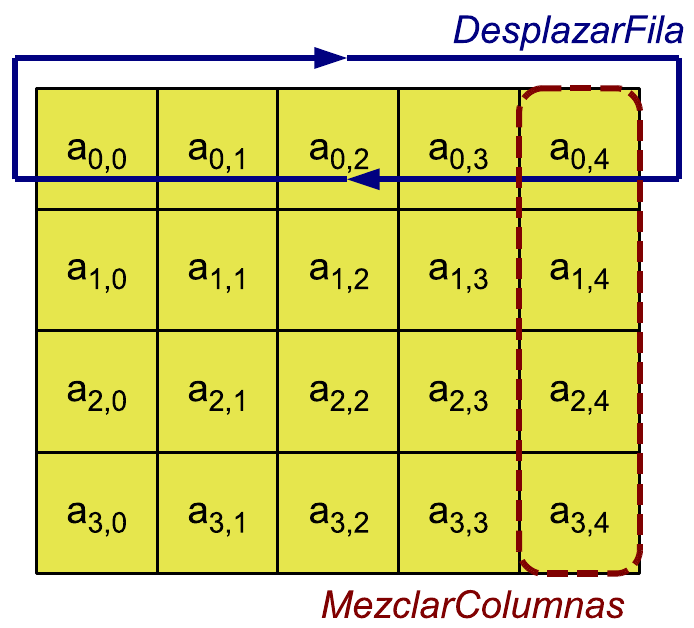
\includegraphics[scale=0.4]{imagenes/aesdesplazarmezclar.png} 
			\caption{Esquema de las funciones $MezclarColumnas$ y $DesplazarFila$ \cite{En2011}}
			\label{desplazarymezclar}
		\end{figure}
%\newpage
	\subsubsection{MezclarColumnas}
	Durante la aplicación de esta función cada columna del vector de estado es vista como una matriz $4 \times 1$ donde sus coeficientes pertenecen a $\mathbb{F}_{256}$. Aplicar MezclarColumnas a cada estado equivale a multiplicar cada columna por la matriz $4 \times 4$.

			\begin{center}
					\begin{pmatrix} 
						02 & 03 & 01 & 01 \\
						01 & 02 & 03 & 01 \\
						01 & 01 & 02 & 03 \\
						03 & 01 & 01 & 02 \\
					\end{pmatrix}
			\end{center}

\section{Cálculo de las Subclaves}
Las subclaves $K_i$ se obtienen de la clave principal $K$ mediante el uso de dos funciones: una de expansión y otra de selección. Siendo $n$ el número de rondas que se van a aplicar, la función de expansión obtiene a partir del valor de $K$ una secuencia de $4(n+1)N_b$ bytes.\\
La función de selección toma consecutivamente de la secuencia obtenida bloques del mismo tamaño que la matriz de estado y los asigna a cada $K_i$.\\

Sea $K(i)$ un vector de bytes de tamaño $4N_k$ conteniendo la clave y sea $W(i)$ un vector de $N_b(n+1)$ registros de 4 bytes, siendo $n$ el número de rondas. 
La función de expansión tiene dos versiones según el valor de $N_k$:

\begin{itemize}
	\item Si $N_k\le6$:
	\begin{algorithm}
		Para $i$ desde 0 hasta $N_{k}-1$ hacer:
		\begin{description}
			$W(i)\leftarrow(K(4·i), K(4·i+1), K(4·i+2), K(4·i+3))$
		\end{description}
		Para $i$ desde $N_k$ hasta $N_{b}·(n+1)$ hacer:\\
			\hspace*{20}$tmp\leftarrow W(i-1)$\\
			\hspace*{20}Si $i \mod N_k = 0$\\
			\hspace*{40}$tmp\leftarrow Sub(Rot(tmp))\oplus Rc(i/N_k)$\\
			\hspace*{20}$W(i)\leftarrow W(i-N_k)\oplus tmp$
	\end{algorithm}
%\newpage
	\item Si $N_k>6$:
	\begin{algorithm}
		Para $i$ desde 0 hasta $N_{k}-1$ hacer:
		\begin{description}
			$W(i)\leftarrow(K(4·i), K(4·i+1), K(4·i+2), K(4·i+3))$
		\end{description}
		Para $i$ desde $N_k$ hasta $N_{b}·(n+1)$ hacer:\\
			\hspace*{20}$tmp\leftarrow W(i-1)$\\
			\hspace*{20}Si $i \mod N_k = 0$\\
			\hspace*{40}$tmp\leftarrow Sub(Rot(tmp))\oplus Rc(i/N_k)$\\
			\hspace*{20}Si $i \mod N_k = 4$\\
			\hspace*{40}$tmp\leftarrow Sub(tmp)$\\
			\hspace*{20}$W(i)\leftarrow W(i-N_k)\oplus tmp$
	\end{algorithm}
\end{itemize}

La función \emph{Sub} devuelve el resultado de aplicar la s-caja de AES a cada uno de los bytes del registro de cuatro que se le pasa como parámetro, la función \emph{Rot} desplaza a la izquierda los bytes del registro y \emph{Rc(j)} es una constante que se define como:
\begin{itemize}
	\item $Rc(j)=(R(j),0,0,0)$.
	\item Cada $R(i)$ es el elemento de $\operatorname{GF}(2^8)$ correspondiente al valor $x^{i-1}$ módulo $x^8+x^4+x^3+x+1$.
\end{itemize}


%
\chapter{Criptografía Asimétrica y Curvas Elípticas. RSA y DH}
\label{chap:cinco}

En esta capítulo voy a explicar de los criptosistemas asimétricos usados en las aplicaciones de mensajería hoy en día. Primero describiré el funcionamiento del cifrado RSA y la firma digital usando este. Después explicaré el problema del Logaritmo Discreto y el intercambio de claves \emph{Diffie-Helmman}. Y por último concluiré haciendo una introducción a la teoría de Curvas Elípticas, el problema del Logaritmo Discreto en estas y el intercambio de claves \emph{Diffie-Hellman} usando este cuerpo.\\

\section{Criptosistema de Rivest-Shamir-Adleman, RSA}
RSA es llamado así en honor a sus creadores Ron Rivest, Adi Shamir y Loenard Adleman. Fue desarrollado en 1977. Cabe a destacar que en 1973 se desarrolló en secreto un criptosistema similar por Clifford Cocks para la \emph{Government Communications Headquarters}, que es la agencia de inteligencia de señales británica, y fue desclasificado en 1997\cite{cliffordCocks}.

Dado que tenemos ya las herramientas necesarias vamos a describir el funcionamiento de RSA. El contenido de esta sección se basa en \cite{angelRiosMateos}.\\

\subsection{Funcionamiento de RSA}
El usuario elige dos números primos distintos \emph{p} y \emph{q} de buen tamaño ya que mientras más grandes sean más seguro será el cifrado.
Se calcula $n = pq$ y por tanto tenemos que $\phi(n) = (p-1)(q-1)$. A continuación se elige un elemento $c$ coprimo con $\phi(n)$ y se calcula el inverso $d = c^{-1}\mod \phi(n)$. La clave pública será $k=(n,c)$ y la clave privada $k'=(n,d)$.

En un principio se consideraba que un tamaño de $n$ de 1024 bits era lo suficientemente grande para que fuera seguro, pero en 2003 Tromer y Shamir mostraron que es posible factorizar números de 1024 bits \cite{1024RSA} por lo que en la actualidad se considera 2048 bits como un tamaño seguro.

El conjunto de los mensajes sin cifrar es $\mathcal{M}$, el de los mensajes cifrados será $\mathcal{C}$ y se verifica que $\mathcal{M} = \mathcal{C} = \mathbb{Z}_n$. Las funciones de cifrado y descifrado son respectivamente:
\begin{align*}
	E_{k}:\mathcal{M}\rightarrow\mathcal{C},\\
	a \rightarrow a^c,
\end{align*}
\begin{align*}
	D_{k'}:\mathcal{C}\rightarrow\mathcal{M},\\
	a \rightarrow a^d.
\end{align*}

Como hemos visto anteriormente, el tamaño del mensaje puede llegar a ser un problema ya que aumenta el tiempo de encriptación y desencriptación. Para solucionar esto se puede fragmentar el mensaje y usar métodos de operación en bloques. Lo más habitual es usar funciones resumen, que de hecho, es el método que se sigue en las aplicaciones de mensajería.

Además RSA puede ser vulnerable en función de los números primos que se elijan y el tamaño de estos. 
Por ejemplo para evitar \textbf{el ataque por módulo común}, es recomendable utilizar distinto módulo $n$ para cada clave. 
Para evitar \textbf{el ataque por exponente pequeño} es recomendable utilizar unos números primos $p$ y $q$ grandes. Ya que si no se usan, se puede utilizar el Teorema Chino del Resto para factorizar $n$ y obtenerlos. 
Para evitar \textbf{el ataque por primos muy próximos} se recomienda usar números primos que estén relativamente alejados entre sí. 

\subsection{Firma digital RSA}
La firma digital con RSA, es una herramienta muy utilizada en las aplicaciones de mensajería para garantizar el no repudio de los mensajes.
Dados dos interlocutores A y B cada uno con sus claves públicas:
\begin{itemize}
	\item para A tenemos $n_A$, $d_A$ y $c_A$,  
	\item para B tenemos $n_B$, $d_B$ y $c_B$.  
\end{itemize}
Para que B sepa que un mensaje \emph{m} ha sido enviado por A se siguen los siguientes pasos.
\begin{enumerate}
	\item A cifra el mensaje \emph{m} usando su clave secreta:
		$$
			S=D_A(m)=m^{d_A} \mod n_A.
		$$
	\item A continuación encripta el mensaje firmado con la clave pública de B:
		$$
			C_B(S)=S^{c_B}\mod n_B.
		$$
		y se lo envía a B.
	\item B recibe $C_B(S)=S^{c_B} \mod n_B$ y lo desencripta: 
		$$
			D_B(S^{c_B})=S \mod n_B.
		$$
	\item Una vez desencriptado la primera parte, B desencripta S con la clave pública de A:
		$$
			C_A(S)=C_A(D_A(m))=(m^{d_A})^{c_A}=m^{d_Ac_B}=m^{1+k\phi(n_A)}\equiv m \mod n_A.
		$$
\end{enumerate}

Una vez hecho esto, B podría afirmar casi con total seguridad que el mensaje ha sido enviado por A garantizando el no repudio del mensaje.

Sin embargo este método tiene un inconveniente y es que para documentos muy largos, el proceso para firmar y verificar es muy lento. Para solucionarlo se utiliza una función hash o resumen de manera que en lugar de firmar el mensaje entero, se firma un resumen de este. La firma en este caso quedaría $fir(m)=h(m)^{d_A} \mod n$ y la comprobación sería $h(m)=fir(m)^{d_A} \mod n$ donde $h$ es una función hash o resumen.

\section{El Problema del Logaritmo Discreto. Diffie-Hellman}
El intercambio de claves \emph{Diffie-Hellman} es un método basado en el Problema del Logaritmo Discreto muy utilizado en las aplicaciones de mensajería al iniciar una conexión. La información de este apartado sobre el logaritmo discreto ha sido obtenida de \cite{angelRiosMateos} y la de \emph{Diffie-Hellman} ha sido obtenida de \cite{En2011}.

El Problema del Logaritmo Discreto es definido de la siguiente forma:
\begin{definicion}
	Sea S un semigrupo finito. El Problema del Logaritmo Discreto en el semigrupo S es el de resolver una ecuación del tipo\\
		$$
			a^x\!=b\;(x\in \mathbb{N}),
		$$
	donde a y b son dos elementos dados de S.
\end{definicion}

La complejidad del Problema del Logaritmo Discreto depende en gran medida del semigrupo $S$ que se elija.
Dado que si se eligiera como $S$ el grupo aditivo $\mathbb{Z}_n$ la solución se obtendría fácilmente resolviendo una ecuación de congruencias del tipo $aX \equiv b \mod n$ que equivaldría a resolver la ecuación diofántica $aX + nY = b$. Pero si ahora $S$ pasara a ser los semigrupos multiplicativos $\mathbb{Z}_n$ o $\mathbb{F}_q$ o sus grupos de unidades, el problema aumentaría su complejidad de manera significativa.

Se cree que el problema de logaritmo discreto es $\mathbb{NP}$-completo pero todavía no ha sido demostrado por lo que se considera un problema $\mathbb{NP}$-Intermedio. Estos problemas son llamados así porque no están dentro de los problemas $\mathbb{P}$ ni en los problemas $\mathbb{NP}$-completo \cite{NP-intermedio}.

Una vez visto el problema de logaritmo discreto, se explicará el intercambio de claves \emph{Diffie-Hellman}.
\subsection{Intercambio de claves Diffie-Hellman}
Antes de explicar el intercambio de claves \emph{Diffie-Hellman} se introducirá el problema de Diffie-Hellman ya que es la base de este.\\

\begin{definicion}
		(El Problema Diffie-Hellman)\\ Dado un número primo p, un número $\alpha$ que sea un \emph{generador} de $\mathbb{Z}_{p}\setminus\{0\}$, $\alpha^a$ y $\alpha^b$, encontrar $\alpha^{ab} \mod p$.  
\end{definicion}

\subsubsection{Intercambio de claves \emph{Diffie-Hellman}}
El intercambio de claves \emph{Diffie-Hellman} es un algoritmo asimétrico basado en el problema de \emph{Diffie-Hellman}, empleado para acordar una clave común en un canal inseguro. Los pasos que se siguen son:

Sean $A$ y $B$ dos interlocutores que quieren compartir un valor $K$. Para ello se calcula un número primo $p$ y un generador $\alpha$ de $\mathbb{Z}_{p}\setminus\{0\}$ con $2\leq \alpha \leq p-2$. Esta información es pública y conocida por ambos.
\begin{enumerate}
	\item $A$ escoge un número aleatorio $x$, comprendido entre 1 y $p-2$ y envía a $B$ el valor 
		$$
			\alpha^x \mod p.
		$$
	\item Análogamente $B$ escoge un número aleatorio $y$, comprendido entre 1 y $p-2$ y envía a $A$ el valor 
		$$
			\alpha^y \mod p.
		$$

	\item $B$ recoge $\alpha^x$ y calcula $K=(\alpha^x)^y \mod p$.
	\item $A$ recoge $\alpha^y$ y calcula $K=(\alpha^y)^x \mod p$.
\end{enumerate}
Puesto que $x$ e $y$ son conocidos solamente por $A$ y $B$ respectivamente, tenemos que al final ambos acaban conociendo el valor de $K$.\\

\section{Curvas Elípticas en Criptografía}
A continuación se introducirá la teoría de curvas Elípticas ya que nos permitirá redefinir el intercambio de claves usando estas. Es el método que se usa actualmente en aplicaciones de mensajería que implementan el protocolo \emph{MTProto} y \emph{Signal}.

El uso de la criptografía en Curvas Elípticas está muy extendido en la actualidad.
Esto es debido a sus propiedades que dan lugar a problemas muy complejos y muy similares a los que se tienen en la aritmética modular pero garantizando una complejidad mayor y por ende mayor seguridad. 
El hecho de que generen problemas tan semejante hace que sean utilizadas en algunos algoritmos asimétricos como puede ser el intercambio de claves \emph{Diffie-Hellman} que se verá más adelante. 
Aunque a nivel teórico su estructura algebraica es más compleja que la de la aritmética modular, en la práctica cuando se implementan suelen ser más eficientes. Además tienen la ventaja de que suelen usar claves más cortas.

El uso de curvas elípticas en criptografía se presentó por primera vez en 1985 por Neal Koblitz y Víctor Miller de manera independiente.
La información para esta sección se ha obtenido de \cite{En2011} y de \cite{apuntesCriptografia}.

Una curva elíptica $E$ sobre un cuerpo $\mathcal{K}$ es el conjunto de los $(x,y)\in \mathcal{K}^2$ tales que
$$
	y^2+a_1xy+a_3y = x^3+a_2x^2+a_4x+a_6,
$$
junto con un punto $\mathcal{O}$.

Un ejemplo de representación curvas elípticas en $\mathbb{R}$ se puede apreciar en la siguiente figura.
\begin{figure}[htb]
	\centering
	\subfloat[\centering Curva $y^2=x^3-4x+1$]{{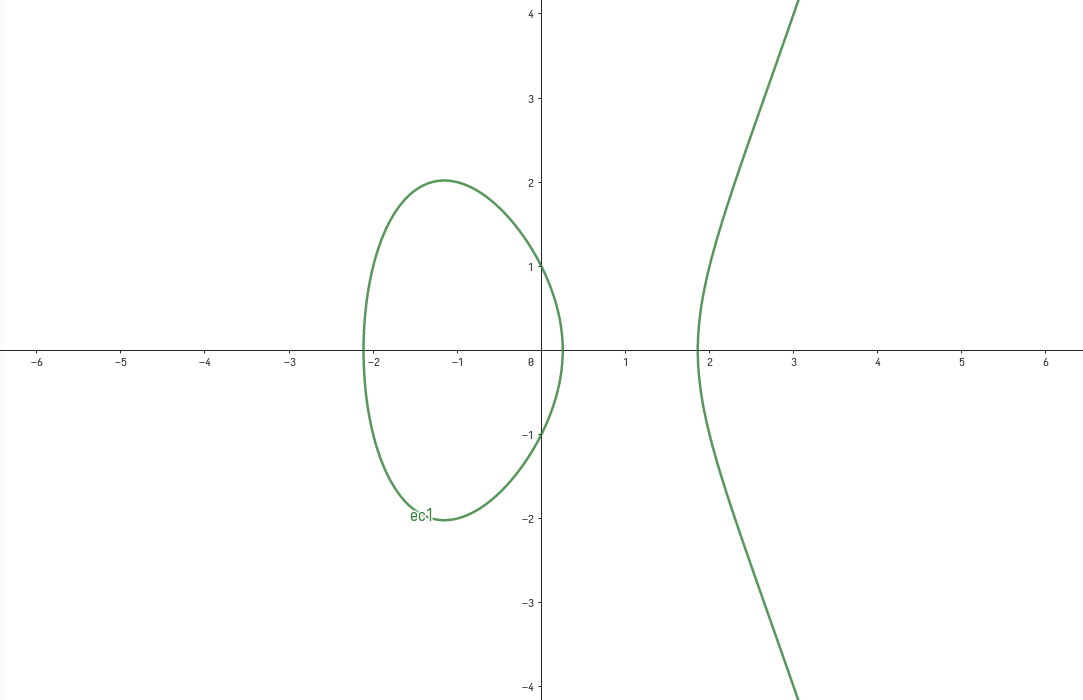
\includegraphics[width=5.9cm]{imagenes/ec1:y^2x^3-4x+1.png}}}
	\qquad
	\subfloat[\centering Curva $y^2=x^3-3x+4$]{{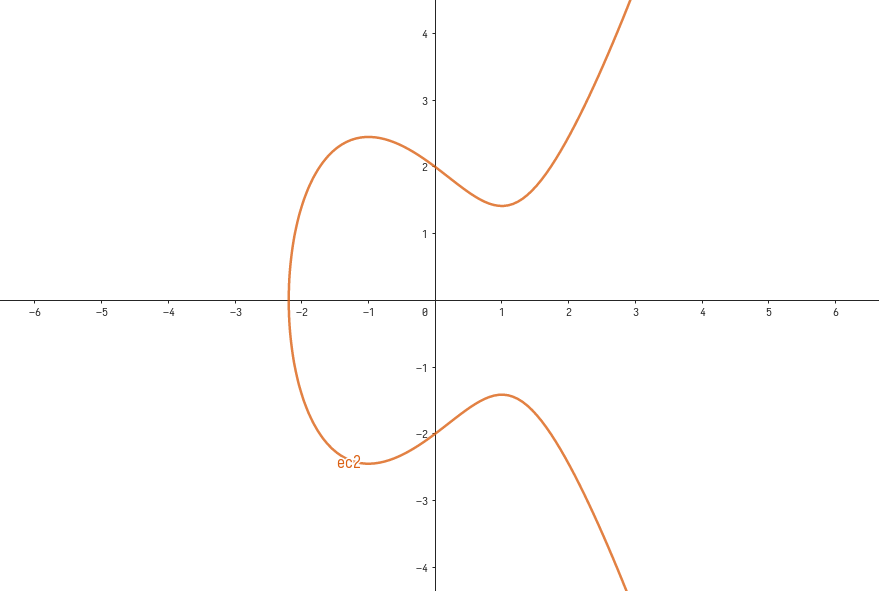
\includegraphics[width=5.9cm]{imagenes/ec2:y^2x^3-3x+4.png}}}
\end{figure}

\begin{proposicion}
		Sea $p=\operatorname{char}(\mathcal{K})$ y sea $E$ una curva elíptica definida sobre $\mathcal{K}$.
		\begin{enumerate}
			\item Si $p$\textgreater$3$, la ecuación $E$ puede simplificarse a
		\begin{align}
			y^2=x^3+ax+b,\label{eq:tipo1}
		\end{align}
		recibiendo el nombre de forma de Weiertrass.
			\item Si $p=3$, la ecuación de $E$ puede simplificarse a 
		\begin{equation}
			y^2=x^3+a^2+bx+c.
		\end{equation}
			\item Si $p=2$ la ecuación de $E$ puede simplificarse a 
				\begin{align}
					y^2+xy=x^3+ax^2+b \: si\: a_1 \neq 0,\label{eq:uno}\\
					y^2+ay=x^3+bx+c \: si\: a_1=0,\label{eq:dos}
				\end{align}
		también se denominan como forma de Weiertrass.
		\end{enumerate}
\end{proposicion}

Las curvas más utilizadas en criptografía son las curvas definidas sobre $\mathbb{Z}_p$ del tipo \eqref{eq:tipo1} y las curvas sobre $\mathbb{F}_{2^l}$ con un $l$ grande y verificando \eqref{eq:uno}. Me voy centrar en explicar estas últimas porque actualmente en las aplicaciones de mensajería son las que se utilizan.

\begin{proposicion}
	Una curva $E(x,y)$ sobre $\mathbb{F}_{2^l}$ que satisface \eqref{eq:uno} tiene un punto singular si y solo si $b=0$.
\end{proposicion}
\begin{proof}
	Sea $F(x,y)=y^2+xy+x^3+ax^2+b$. $E$ es singular en $(x_0,y_0)\in E$ si y solo si  
	$$
		\frac{\partial F}{\partial x}(x_0,y_0)=\frac{\partial F}{\partial y}=0.
	$$
	Dado que
	$$
		\frac{\partial F}{\partial x} = y+3x^2+2ax=y+x^2
	$$
	y
	$$
		\frac{\partial F}{\partial y}=2y+x=x,
	$$
	el único punto donde puede haber una singularidad es $(0,0)$ que pertenece a la curva si y solo si $b=0$.
\end{proof}

\begin{lema}
	Sea $E=E(a,b)$ una curva sobre $\mathbb{F}_{2^l}$ definida por la ecuación \eqref{eq:uno}. Si $(x_0,y_0), (x_1,y_1)\in E$, entonces $y_1=y_0$ o $y_1=x_0+y_0$.
\end{lema}
\begin{proof}
	Como se cumple que
	$$
		y_0^2+x_0y_0=x_0^3+ax_0^2+b=y_1^2+x_0y_1,
	$$
	tenemos que
	$$
		(y_1+y_0)^2=y_1^2+y_0^2=(y_1+y_0)x_0.
	$$
	Si $y_0\neq y_1$ tenemos que $y_0+y_1\neq0$ y por tanto $x_0=y_1+y_0$, luego $y_1=y_0$ o $y_1=y_0+x_0$.
\end{proof}

\begin{proposicion}
	Sea $E(a,b)$ una curva elíptica sobre $\mathbb{F}_{2^l}$ que verifica \eqref{eq:uno}. Sean $P=(x_0,y_0),\: P_1=(x_1,y_1)\:y\:P_2=(x_2,y_2)$ puntos de $E(a,b)$. Entonces, 
	\begin{enumerate}
		\item $-P=(x_0,x_0+y_0)$.
		\item Si $P_2=-P_1,\: P_1+P_2=\mathcal{O}$.
		\item Si $P_2\neq-P_1,\:P_1+P_2=P_3,$ viene dado por
		\begin{equation}
			\begin{split}
					P_3 &=(x_3,y_3)\notag\\
						&=(m^2+m+a+x_1+x_2,m(x_1+x_3)+x_3+y_1)\notag,
			\end{split}
		\end{equation}
		donde 
		\begin{equation}
		  m =
			\begin{cases}
				(y_2+y_1)(x_2+x_1)^{-1} & \text{si } x_1\neq x_2, \\
				x_1+y_1x_1^{-1} & \text{si } x_1=x_2
			\end{cases}       
			\notag
		\end{equation}
	\end{enumerate}
\end{proposicion}
\begin{proof}
	La ecuación \eqref{eq:tipo1} es un caso particular de \eqref{eq:uno} tomando $a_1=1$, $a_3=0$, $a_2=a$, $a_4=0$ y $a_6=b$. Luego la aritmética es consecuencia de la aritmética definida para una curva elíptica cualquiera, por el lema visto anteriormente, tenemos que $x_1=x_2$ y $P_2\neq-P_1$ implica $P_2=P_1$ y por tanto $P_1+P_2=2P_1$.
\end{proof}

\subsection{Uso de las Curvas Elípticas en criptografía}
Una vez introducidas las Curvas Elípticas y visto unos resultados necesarios para este apartado, voy a explicar los elementos que se necesitan para poder usar las Curvas Elípticas en criptografía.

Para poder utilizarlas necesitaremos los siguientes parámetros.
\begin{itemize}
	\item El cuerpo base sobre el que se definirán las curvas, $\mathbb{F}_q$
	\item Los parámetros $a,b \in \mathbb{F}_q$, que serán los que definan la curva $E$ a partir de las ecuaciones \eqref{eq:tipo1} y \eqref{eq:uno}.
	\item Un punto base $Q\in E$ cuyo orden es $n$ el cual será un primo grande.
	\item El cofactor $h$ tal que $|E|=hn$. Las curvas que satisfacen esto y además $n$ es primo y $h$ pequeño se denominan \emph{curvas de orden próximo a primo} y $E_n$ es el \emph{subgrupo de orden primo}.	
\end{itemize}

\begin{lema}
		Sea $E$ una curva elíptica tal que $|E|=hn$ con $n$ primo y $h$\textless $n$. Entonces $E$ tiene un único subgrupo $E_n$ de orden $n$ que es cíclico y generado por cualquiera de sus elementos distintos de $\mathcal{O}$.
\end{lema}
\begin{proof}
		Por el Teorema de Cassel, $E\cong \mathbb{Z}_{d_1}\times \mathbb{Z}_{d_2}$, con $d_1\:|\:d_2$. Como $h$\textless$n$ se cumple que $n\:|\:d_2$ pero $n \nmid d_1$. Luego $E_n$ se corresponde con el subgrupo $\{0\}\times \langle \frac{d_2}{n} \rangle\leq\mathbb{Z}_{d_1}\times\mathbb{Z}_{d_2}$.
\end{proof}

Una vez visto esto quedaría ver la selección de la curva a utilizar, ya que como se verá a continuación, no sirve cualquiera. Esto es debido a que necesitamos que el problema del logaritmo discreto sea difícil, es decir, que sea computacionalmente muy costoso de romper.

Las familias de curvas que generalmente se evita utilizar en criptografía son las siguientes.
\begin{itemize}
	\item \emph{Curvas supersingulares}, como pueden ser las que tienen la forma \eqref{eq:dos}. En estas curvas se cumple que $E_n\cong \mathbb{F}_{q^l}^*$ con $l$ pequeño. Esto fue demostrado por Menezes-Okamoto-Vanstone empleando el \emph{par de Weil}. Para solucionar esto habría que ver que $n\nmid q^l-1$ para valores pequeños de $l$.
	\item Curvas sobre $\mathbb{F}_p$ tales que $|E|=p$. Esta familia es problemática ya que se puede construir un isomorfismo $E\cong\mathbb{F}_p$ mediante un algoritmo en tiempo polinomial, solucionado el problema del logaritmo discreto mediante el uso del algoritmo de Euclídes extendido en $\mathbb{F}_p$.
\end{itemize}

Teniendo en cuenta esto, la curva debe elegirse mediante una búsqueda aleatoria para evitar centrarse en familias que en un futuro pudieran pasar a ser inseguras. Por lo que el proceso sería elegir los parámetros $a,b\in \mathbb{F}_q$. A continuación se calcula $|E(a,b)|$ y se comprueba si $|E(a,b)|=hn$ para $h$ pequeño y $n$ un número primo. Por último se tiene que ver su resistencia frente a los ataques anteriores.

La parte más compleja del procedimiento es calcular el orden de la curva. Pero para ello podemos usar el Teorema de Hasse el cual nos da una cota de este.
\begin{teorema}
	(Hasse). Sea $E$ una curva elíptica sobre $\mathbb{F}_q$ dada por \eqref{eq:tipo1} y sea $t=q+1-|E|$. Entonces
	$$
		|t|\leq2\sqrt{q}.
	$$
\end{teorema}
Gracias a un algoritmo desarrollado por Schoof-Elkies-Atkin para cuerpos primos y a Satoh para cuerpos binarios permite calcular dicho orden en tiempo polinomial.

Para calcular los puntos de la curva tenemos que, para una curva elíptica $E=E(a,b)$ definida sobre $\mathbb{F}_q$ el morfismo
$$
	\pi:E\backslash\{\mathcal{O}\}\rightarrow\mathbb{F}_q,\: (x,y)\mapsto x,
$$
no es sobreyectivo. Esto hace que no todos los elementos de $\mathbb{F}_q$ son primera coordenada de un punto de la curva.\\

\textbf{Caso $\mathbb{F}_p$}\\
La curva es del tipo \eqref{eq:tipo1}, por lo que debemos buscar valores $x_0\in \mathbb{F}_p$ que verifiquen $x_0^3+ax_0+b$ es un cuadrado perfecto. Por lo que necesitamos decidir si $\beta\in\mathbb{F}_p$ es residuo cuadrático y, en caso de serlo, calcular sus raíces. Gracias al Criterio de Euler podemos simplificar esta tarea. 
\begin{lema}
		(Criterio de Euler). $\beta \in \mathbb{F}_p$ es residuo cuadrático si y solo si $\beta^{\frac{p-1}{2}}\equiv 1 \mod p$.
\end{lema}
\textbf{Caso $\mathbb{F}_{2^l}$}\\
En este caso la curva elíptica $E=E(a,b)$ viene dada por la ecuación \eqref{eq:uno}. Si $(x_0,y_0)\in E$, $y_0$ es solución de la ecuación cuadrática
$$
	y^2+x_0y=x_0^3+ax_0^2+b.
$$

Para elegir el punto base, seleccionamos aleatoriamente $P\in E$ donde $E=E(a,b)$ es una curva elíptica tal que $|E|=hn$ con $n$ primo y $h$ pequeño. Una vez seleccionado calculamos $Q=hP$ y comprobamos si $Q\neq\mathcal{O}$. Como $n$ es primo y $nQ=\mathcal{O}$, $Q$ será un generador de $E_n$. Si $Q=\mathcal{O}$ tomamos un nuevo $P$ y repetimos la operación.

Con esto ya tenemos todo lo necesario para explicar el Problema del Logaritmo Discreto usando Curvas Elípticas.
\section{El Problema del Logaritmo Discreto usando Curvas Elípticas. \emph{Diffie-Hellman}}
En esta sección voy a describir el análogo del Problema del Logaritmo Discreto en Curvas Elípticas y como resultado un análogo del intercambio de claves \emph{Diffie-Hellman}.

\subsection{El Problema del Logaritmo Discreto en Curvas Elípticas}
Para todo punto $p$ definido en una curva elíptica, se define $\langle p\rangle$ al conjunto $\{\mathcal{O}, p, 2p, ... \}$.
En $E(\operatorname{GF}(n))$ y $E(\operatorname{GF}(2^n))$ los conjutos como los que se han definido, tienen que ser finitos ya que los puntos de las curvas son finitos. Luego para todo punto $q\in \langle p\rangle$ tiene que existir un número $k \in \mathbb{Z}$ que verifique que $kp=q$.

Por lo tanto, el problema del logaritmo discreto en curvas elípticas consiste en hallar dicho número $k$ a partir de $p$ y $q$.
\subsection{Intercambio de claves \emph{Diffie-Hellman} en curvas elípticas}
Una vez visto el Problema del Logaritmo Discreto en Curvas Elípticas, voy a explicar el intercambio de claves \emph{Diffie-Hellman} usando Curvas Elípticas. Para ello se explicaré previamente la conjetura \emph{Diffie-Hellman} en Curvas Elípticas. La información de este apartado la he obtenido de \cite{apuntesCriptografia}.

Fijamos una curva elíptica $E=E(a,b)$ tal que $|E|=hn$ con $n$ primo y $h$ pequeño como he explicado en la sección anterior. Esta curva puede estar definida sobre $\mathbb{F}_p$ o sobre $\mathbb{F}_{2^l}$. También se fija  $q$ un elemento de orden $n$, en función del cuerpo que elijamos lo fijamos de una forma u otra como ya hemos visto.
\begin{definicion}
	(Conjetura Diffie-Hellman). Conocidos $p_a=aq$ y $p_b=bq$ para ciertos $1\leq a,\: b\leq n$, calcular $abq$ es equivalente a nivel computacional a calcular $a=\log_q(p_a)$ o $b=\log_q(p_b)$.
\end{definicion}
El protocolo de intercambio de claves queda como sigue.\\
Dadas dos personas A y B que quieren realizar un intercambio de claves.
\begin{itemize}
	\item A y B se ponen de acuerdo en la curva elíptica $E$ y el punto $q\in E$.
	\item A elige aleatoriamente un número $a\in\{2,\dots,n-1\}$ y le envía a B $p_a=aq$.
	\item B elige aleatoriamente un número $b\in\{2,\dots,n-1\}$ y le envía a A $p_b=bq$.
	\item A calcula $a(p_b)$.
	\item B calcula $b(p_a)$.
	\item La clave compartida es $(ab)q=a(p_b)=b(p_a)$.
\end{itemize}


%
\chapter{Funciones Hash}
\label{chap:seis}

En este capítulo voy a describir que son las funciones hash, como construirlas usando la construcción \emph{Merkle-Damgård} y por último explicaré las funciones hash más utilizadas en las aplicaciones de mensajería en la actualidad.
\section{¿Que son las funciones hash?}
Una función resumen o función hash es una función que se puede calcular mediante un algoritmo en el cual se transforma un conjunto arbitrario de datos en una nueva serie de caracteres con una longitud fija independiente del tamaño de los datos de entrada.
Estas funciones son muy utilizadas en criptografía ya que como hemos visto, en el caso de RSA el tamaño del bloque puede suponer un problema debido a que aumenta considerablemente el tiempo de ejecución.
Para ello se utilizan funciones hash, ya que mediante el uso de estas, se consigue reducir el tamaño del mensaje sin perder información.\\ La información para esta sección la he obtenido \cite{aepd}.

Las propiedades esperadas de una función hash son:
\begin{itemize}
	\item Se tiene que poder utilizar en contenido digital de cualquier tamaño y formato.
	\item Independientemente del tamaño de la entrada y del tipo, se produce una salida numérica de tamaño fijo.
	\item Para el mismo conjunto de datos de entrada, el resultado siempre es el mismo.
	\item Reconstruir el mensaje original a partir del generado tiene que ser muy complejo, idealmente imposible.
	\item Una variación mínima del mensaje original tiene que producir un hash totalmente distinto, esta propiedad se denomina \emph{difusión}.
	\item Dado un mensaje, tiene que ser muy difícil encontrar otro mensaje con la misma imagen que este, recibe el nombre de \emph{colisión débil}.
	\item Tiene que ser muy costoso encontrar dos mensajes que tengan la misma imagen, esta propiedad es denominada \emph{colisión fuerte}.
	\item Dado un posible valor del espacio imagen, tiene que ser igual de probable que salga este u otro cualquiera. Es decir todos los valores tienen la misma probabilidad de salir.
\end{itemize}

Visto esto, en general, una función hash funciona de la siguiente forma:
\begin{enumerate}
	\item El mensaje de entrada se divide en bloques.
	\item Una fórmula calcula el hash, un valor con un tamaño fijo, para el primer bloque.
	\item Se calcula el hash del siguiente bloque y se suma con el hash calculado previamente.
	\item Se repite de manera análoga con el resto de bloques hasta que se recorren todos.
\end{enumerate}

Las hash que explicaré serán: \emph{SHA-0} y \emph{SHA-1} que son las funciones antecesoras de la función \emph{SHA-256} que es la que se utiliza mayoritariamente en las funciones de mensajería en la actualidad. Algunas también pueden utilizar SHA-1.

\section{La construcción \emph{Merkle-Damgård}}
Antes de desarrollar las funciones hash mencionadas anteriormente, voy a describir la construcción \emph{Merkle-Damgård}. Este es un método para construir funciones hash que sean resistentes a colisiones a partir de funciones de compresión unidireccionales. La información para este apartado ha sido obtenida de \cite{Tiwari2017}.

Este método fue descubierto en 1989 por Merkle y Damgård de manera independiente. Es muy importante ya que gracias a este, se desarrollaron las funciones hash \emph{MD4,\:MD5,\:SHA-0,\:SHA-1 \text{ y }SHA-2} entre otras.

Una función de compresión es una función que toma una entrada de longitud fija y produce un resumen de longitud fija. Esta recibe dos entradas: una variable cadena y un bloque del mensaje.

\begin{figure}[htb]
	\centering
	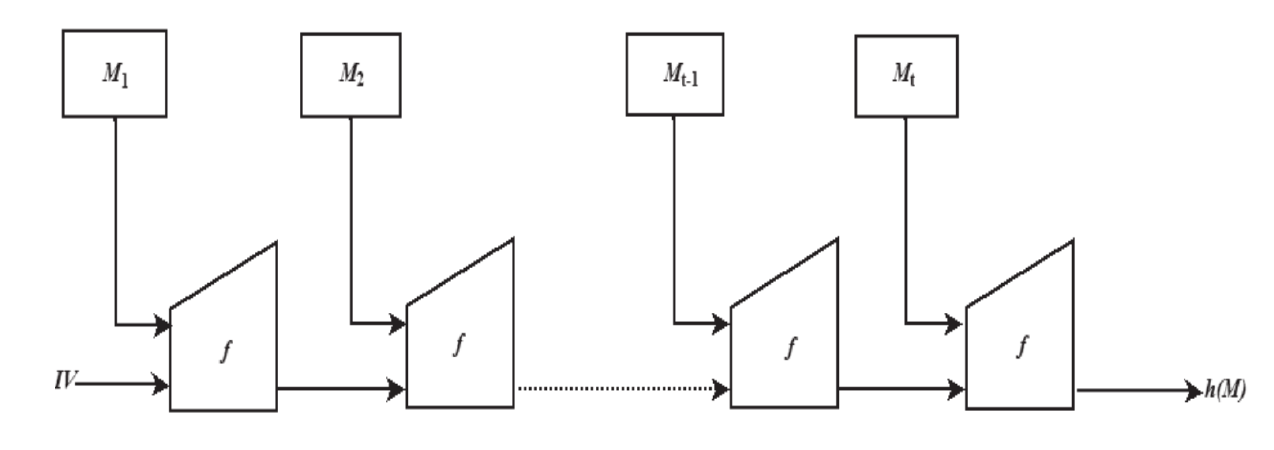
\includegraphics[scale=0.3]{imagenes/md1.png} 
	\caption{Construcción de Merkle-Damgård \cite{Tiwari2017}.}
\end{figure}
Sea $f:\{0,1\}^b\times\{0,1\}^n\rightarrow\{0,1\}^n$ una función de compresión que toma un bloque de mensajes de $b$ bits y un valor de encadenamiento de $n$ bits. Sea $h:\{0,1\}^*\rightarrow\{0,1\}^n$ una construcción \emph{MD} construida iterando la función de compresión $f$ para procesar un mensaje de longitud arbitraria. Para que esto sea posible lo que se hace es rellenar cualquier mensaje para que la longitud de este sea múltiplo de la longitud de bloque $b$ de $f$.

El relleno se realiza añadiendo después del último bit del último bloque del mensaje un único bit $1$ seguido del resto de bits necesarios a $0$.
Por último, para terminar de rellenar el mensaje, se añade la codificación binaria de la longitud del mensaje.\\
Una vez rellenado el mensaje, la entrada se divide en $t$ bloques, cada uno de longitud $b$. La función hash resultante puede describirse de la siguiente manera.
$$
		H_0 = IV,
$$
$$
		H_i = f(H_{i-1},M_i)\:i=1\dots t,
$$
$$
		h(M)=H_t.
$$

Este proceso se continua recursivamente, actualizando la variable cadena a partir de pasar cada bloque del mensaje por la función de compresión. La salida será la variable cadena. En \ref{mdcon} se puede ver un resumen del proceso.

\begin{figure}[htb]
	\centering
	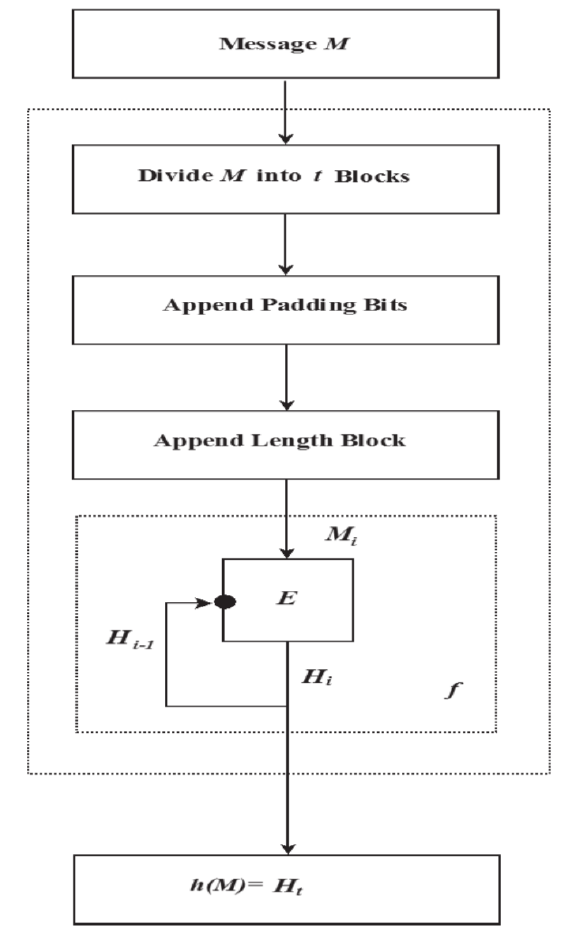
\includegraphics[scale=0.4]{imagenes/md2.png} 
	\caption{Esquema de los pasos seguidos en la construcción de Merkle-Damgård \cite{Tiwari2017}.}
	\label{mdcon}
\end{figure}
\newpage
\section{SHA-0}
SHA-0 es una función hash que apareció publicada en el Federal Information Processing Standard (FIPS-180) por el NIST en 1993 \cite{Penard2008}. Está basada en \emph{MD4} y \emph{MD5}. El algoritmo transforma un mensaje de cualquier tamaño hasta $2^{64}$ bits y los transforma en un resumen de 160 bits.

El funcionamiento de SHA-0 es el siguiente \cite{sha0}:
\begin{enumerate}
	\item Al igual que en MD5, el mensaje se rellena con un único bit '1' seguido de 0-511 bits '0'. A continuación se añade una representación de 64 bits de la longitud del mensaje donde el número de ceros es elegido para asegurar que la longitud total del mensaje es un múltiplo de 512 bits. El mensaje se divide en bloques de 512 bits: $M_1,...,M_n$.
	\item Para la primera iteración se utiliza un búffer predefinido:
	$$
		h_0=(67452301_x, EFCDAB89_x, 98BADCFE_x, 10325476_x, C3D2E1F0_x).
	$$
	\item Cada bloque $M_j$ es pasado por la función de compresión junto con el valor actual de $h_{j-1}$, la salida es el nuevo valor de $h_j$, la operación se puede resumir en
	$$
		h_j=compresión(M_j,h_{j-1}).
	$$
	\item $h_n$ es la salida de la función hash.
\end{enumerate}
Los pasos seguidos en la función de compresión son:
\begin{enumerate}
	\item Se divide el bloque $M_j$ de 512 bits en bloques 16 bloques de 32 bits $W_0,W_1,...,W_{15}$. 
	\item Se expanden los 16 bloques de 32 bits en 80 bloques a partir de la siguiente ecuación en recurrencias:
	$$
		W_i=W_{i-3}\oplus W_{i-8}\oplus W_{i-14}\oplus W_{i-16},\; i=16,...,79.
	$$
	Esta expansión se nota como exp(.).
	\item Divide $h_{j-1}$ en 5 registros \emph{A, B, C, D} y \emph{E} como:
	$$
		h_{j-1} = (A_0, B_0, C_0, D_0, E_0).
	$$
	\item Para $i=0,...,79$ hacemos:
	$$
		A_{i+1}=(A_i\lll5)+f_i(B_i,C_i,D_i)+E_i+K_i) \mod 2^{32},
	$$
	$$
		B_{i+1}=A_i,\: C_{i+1}=(B_i\lll30),\: D_{i+1}=C_i,\: E_{i+1}=D_i.
	$$
	Donde las funciones y las constantes están definidas en la tabla \ref{tablasha0}.
	\item La salida de la función sería:
	$$
		h_n=(A_0+A_{80}, B_0+B_{80}, C_0+C_{80}, D_0+D_{80}, E_0+E_{80}).
	$$
\end{enumerate}

\begin{table}[H]
	\begin{center}
		\begin{tabular}{| l | l | l |}
				\hline
				Rondas & $f_i(B,C,D)$ & $K_i$\\ \hline
				$0\leq i\leq 19$ & $BC\vee BD$ & $5AD9EBA1_x$\\ \hline
				$20\leq i\leq 39$ & $B\oplus C\oplus D$ & $6ED9EBA1_x$\\ \hline
				$40\leq i\leq 59$ & $BC\vee BD\vee CD$ & $8F1BBCDC_x$\\ \hline
				$60\leq i\leq 79$ & $B\oplus C\oplus D$ & $CA62C1D6_x$\\ \hline
		\end{tabular}
		\caption{Funciones y constantes usadas en la función de compresión de SHA-0 \cite{sha0}.}
	\label{tablasha0}
	\end{center}
\end{table}

\section{SHA-1}
La función SHA-1 es una función hash diseñada en 1995 por la \emph{National Security Agency} (NSA) dado que que se encontraron varias colisiones y vulnerabilidades en la función SHA-0 \cite{Penard2008}.

Su funcionamiento es muy similar al de la función SHA-0 variando en las funciones y variables usadas en las distintas rondas de la función de compresión. En la tabla \ref{tablasha1} se pueden ver los nuevos valores utilizados.

\begin{table}[htb]
	\begin{center}
		\begin{tabular}{| l | l | l |}
				\hline
				Rondas & $f_i(B,C,D)$ & $K_i$\\ \hline
				$0\leq i\leq 19$ & $(B\wedge C)\oplus (\overline{B}\wedge D)$ & $5A827999_x$\\ \hline
				$20\leq i\leq 39$ & $B\oplus C\oplus D$ & $6ED6EBA1_x$\\ \hline
				$40\leq i\leq 59$ & $(B\wedge C)\oplus (B\wedge D) \oplus (C\wedge D)$ & $8FABBCDC_x$\\ \hline
				$60\leq i\leq 79$ & $B\oplus C\oplus D$ & $CA62C1D6_x$\\ \hline
		\end{tabular}
		\caption{Funciones y constantes usadas en la función de compresión de SHA-1 \cite{sha1}.}
		\label{tablasha1}
	\end{center}
\end{table}

En imagen \ref{sha01img} se puede observar un esquema del proceso para obtener un el hash seguido por las funciones  SHA-0 y SHA-1 donde \textbf{F} será la función de compresión.
\begin{figure}[htb]
	\centering
	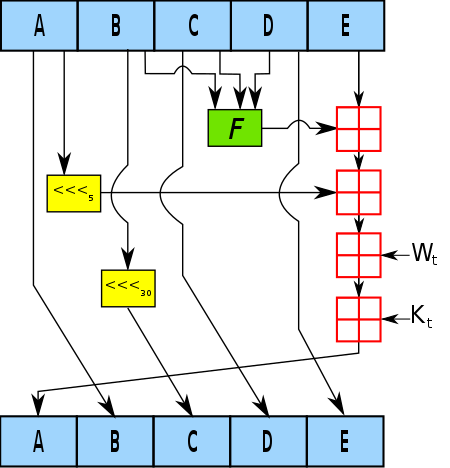
\includegraphics[scale=0.5]{imagenes/sha0-1.png} 
	\caption{Esquema de los pasos seguidos en SHA-0 y SHA-1 \cite{fotosha10}.}
	\label{sha01img}
\end{figure}

\section{SHA-256}
La función SHA-256 pertenece a la familia SHA-2 que es un conjunto de funciones hash diseñadas por la NSA en 2001 \cite{Penard2008}. Esta familia está compuesta por las funciones SHA-224, SHA-256, SHA-384 y SHA-512 donde el número del final indica el tamaño de bloque en el que se dividirá el mensaje. Nos centraremos en la función SHA-256 que como he comentado anteriormente es la que se utiliza en las aplicaciones de mensajería actualmente.

El funcionamiento de las función es el siguiente\cite{Function2016}:

\begin{enumerate}
	\item Al igual que en SHA-0 y SHA-1 se rellena el mensaje de la misma manera y se fragmenta en bloques de 512 bits: $M_1,...,M_n$.
	\item Para la primera iteración se utiliza un búffer predefinido:
	$$
		h_0=(H_1, H_2, H_3, H_4, H_5, H_6, H_7, H_8),
	$$
	donde:\\
	$H_1=6A09E776$,\\
	$H_2=BB67AE85$,\\
	$H_3=3C6EF372$,\\
	$H_4=A54FF53A$,\\
	$H_5=510E527F$,\\
	$H_6=9B05688C$,\\
	$H_7=1F83D9AB$,\\
	$H_8=5BE0CD19$.\\
	\item Cada bloque $M_j$ es pasado por la función de compresión junto con el valor actual de $h_{j-1}$, la salida es el nuevo valor de $h_j$, la operación se puede resumir en:
	$$
		h_j=compresión(M_j,h_{j-1}).
	$$
	\item $h_n$ es la salida de la función hash.
\end{enumerate}
Los pasos seguidos en la función de compresión son:
\begin{enumerate}
	\item Se divide el bloque $M_j$ de 512 bits en bloques 16 bloques de 32 bits $W_0,W_1,...,W_{15}$. 
	\item Se expanden los 16 bloques de 32 bits en 63 bloques a partir de la siguiente ecuación en recurrencias:
	$$
		W_i=\sigma_1(W_{j-2})+W_{j-7}+\sigma_0(W_{j-16}),\; i \in \{16...63\}.
	$$
	\item Divide $h_{j-1}$ en \emph{A, B, C, D, E, F, G} y \emph{H} como:
	$$
		h_{j-1} = (A_0, B_0, C_0, D_0, E_0, F_0, G_0, H_0).
	$$
	\item Para $i=0,...,63$ hacemos:
	$$
		A_{i+1}=H_i+\Sigma_1(E_i)+Ch(E_i,F_i,G_i)+K_j+W_j+\Sigma_0(A_i)+Maj(A_i,B_i,C_i),
	$$
	$$
		B_{i+1}=A_i,\: C_{i+1}=B_i,\: D_{i+1}=C_i,\: F_{i+1}=E_i\: G_{i+1}=F_i,\: H_{i+1}=G_i,
	$$
	$$
		E_{i+1}=D_i+H_i+\Sigma_1(E_i)+Ch(E_i,F_i,G_i)+K_j+W_j.
	$$
	Donde las funciones y las constantes están definidas en la tabla \ref{tablasha0}.
	\item La salida de la función es:
	$$
		h_j=(A_0+A_{63}, B_0+B_{63}, C_0+C_{63}, D_0+D_{63}, E_0+E_{63}, F_0+F_{63}, G_0+G_{63}, H_0+H_{63}).
	$$
\end{enumerate}
Donde tenemos que:
$$
	Ch(x,y,z) = (x\wedge y)\oplus (\overline{x}\wedge z),
$$
$$
	Maj(x,y,z) = (x\wedge y)\oplus (x\wedge z)\oplus (y\wedge z),
$$
$$
	\Sigma_0(x) = (x\ggg2)\oplus (x\ggg13)\oplus (x\ggg22),
$$
$$
	\Sigma_1(x) = (x\ggg6)\oplus (x\ggg11)\oplus (x\ggg25),
$$
$$
	\sigma_0(x) = (x\ggg7)\oplus (x\ggg18)\oplus (x\lll3),
$$
$$
	\sigma_1(x) = (x\ggg17)\oplus (x\ggg19)\oplus (x\lll10).
$$

En la imagen \ref{sha256img} podemos ver un esquema de los pasos seguidos en las funciones SHA-2.

\begin{figure}[htb]
	\centering
	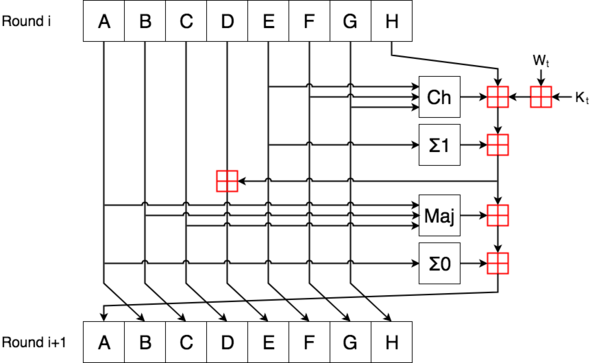
\includegraphics[scale=0.5]{imagenes/sha2.png} 
	\caption{Esquema de los pasos seguidos en las funciones de la familia SHA-2 \cite{sha2wikipedia}.}
	\label{sha256img}
\end{figure}
\newpage
\section{HMAC}
Un \textbf{HMAC} es un código de autenticación usado por algunos criptosis-temas simétricos de bloques que usa una función hash. Puede expresarse como: 

$$
\operatorname{HMAC}_K(m)=h((K^+\oplus opad)||h((K^+\oplus ipad)||m)).
$$

Donde $h$ es la función hash, $K$ es la clave secreta y $K^+$ es el relleno con ceros a la izquierda que se inserta a $K$ para ajustarle el tamaño. Por otro lado tenemos que $ipad$ es el byte 36 en hexadecimal y $opad$ el byte 5C que se repiten para ajustarse al tamaño de $K^+$ \cite{criptografia}.


%
\chapter{Aplicaciones de Mensajería}
\label{chap:siete}

En este capítulo explicaré como usan las aplicaciones de mensajería los criptosistemas que he desarrollado en los capítulos anteriores. Las aplicaciones que he estudiado son: \emph{Telegram}, \emph{WhatsApp}, \emph{Facebook}, \emph{Signal}, \emph{iMessage} y \emph{Line Messenger}.

\section{Telegram (MTProto)}
MTProto es el protocolo de datos con el Telegram cifra sus mensajes. Fue desarrollado por el matemático Nikolái Dúrov y financiado por Pável Dúrov. Al contrario que la mayoría de cifrados, MTProto esta enfocado en ser multisesión e independiente de la plataforma y el transporte de archivos independiente de su formato. MTProto tiene dos versiones.
\begin{itemize}
	\item \textbf{MTProto v1.} En esta versión los mensajes son cifrados con el algoritmo \emph{SHA-1}.
	\item \textbf{MTProto v2.} En 2017 se actualizó MTProto, en esta versión se cambió el cifrado \emph{SHA-1} por \emph{SHA-256} debido a una vulnerabilidad encontrada en \emph{SHA-1}. Esta es la versión que se utiliza actualmente. 
\end{itemize}
La información técnica sobre MTProto que se desarrollará a continuación ha sido obtenida de \cite{Miculan2021} y \cite{WebProto}.

\subsection{Descripción general y resumen de los componentes}
MTProto 2.0 es una suite de protocolos criptográficos diseñados para implementar de manera rápida, escalable y segura intercambio de mensajes sin depositar esa responsabilidad en la seguridad del transporte debajo de dicho protocolo.
El protocolo esta subdividido en tres componentes virtuales independientes.
\begin{itemize}
	\item \textbf{Componente de alto nivel:} Define el método por el cual las consultas de la API y las respuestas se convierten en mensajes binarios. 
	\item \textbf{Capa criptográfica (autorización):} Define el método por el cual los mensajes están cifrados antes de ser enviados a través del protocolo de transporte.
	\item \textbf{Componente de transporte:} Define el método por el cual el cliente y el servidor transmiten los mensajes sobre otro protocolo de red como HTTP, HTTPS, WS, WSS, TCP o UDP.
\end{itemize}
Y se pueden resumir como sigue.\\

\subsubsection{Componentes de alto nivel(Lenguajes de consulta/API RPC)}
Desde el punto de vista del componente de alto nivel, el cliente y el servidor intercambian mensajes dentro de una sesión.

La sesión se adjunta al cliente en lugar de una conexión \emph{websocket/http/https/tcp.} 
Además, cada sesión tiene asociada a clave ID de usuario mediante la cual se logra la autorización.

Pueden estar abiertas varias conexiones a un servidor, los mensajes pueden ser enviados en cualquier dirección a través de cualquiera de las conexiones.
Cuando se usa el protocolo UDP, una respuesta puede ser devuelta por una dirección de IP distinta.

Hay diferentes tipos de mensajes, estos son.
\begin{itemize}
		\item \textbf{Llamadas RPC(cliente-servidor):} Llamadas a los métodos de la API.
		\item \textbf{Respuestas RPC(servidor-cliente):} Resultados de las llamadas RPC.
		\item \textbf{Notificación del estado de los mensajes.}
		\item \textbf{Consultas de estado de mensaje.}
		\item \textbf{Mensaje multiparte o contenedor.}
\end{itemize}
Desde el punto de vista de protocolos de bajo nivel, un mensaje es un flujo de datos alineados con 4 o 16 bytes de límite.
Los primeros campos en un mensaje están fijos y son usados por el sistema criptográfico o de autorización.

Cada mensaje, consiste en un identificador del mensaje \emph{(Message Identifier)} de 64 bits, \emph{número de secuencia del mensaje dentro de una sesión}, \emph{longitud} de 32 bits y \emph{cuerpo del mensaje} de cualquier tamaño, siempre y cuando sea múltiplo de 4. 
Además cuando un contenedor o un mensaje simple se envían, una \emph{cabecera interna} se añade al principio del mensaje, luego el mensaje es cifrado y se le añade una \emph{cabecera externa} la cual será una \emph{clave de identificación} de 64 bits y una \emph{clave del mensaje} de 128 bits.

El \emph{cuerpo} del mensaje normalmente consiste en un \emph{tipo mensaje} de 32 bits seguido de los \emph{parámetros dependientes del tipo}.
Los números están escritos en \emph{little endian}. Sin embargo los números muy grandes (2048 bits) usados en \textbf{RSA} y \textbf{DH} están escritos en \emph{big endian} porque es lo que hace la biblioteca \textbf{OpenSSL}.

\subsubsection{Autorización y Cifrado}
			Antes de que un mensaje sea transmitido por la red usando un protocolo de transporte, este es cifrado añadiendo una cabecera externa la cual es insertada al principio del mensaje y contiene:
	\begin{itemize}
		\item \emph{Key Identifier} de 64 bits,
		\item \emph{Message Key} de 128 bits.
	\end{itemize}
Una clave de usuario junto con una clave de mensaje definen una clave de 256 bits la cual es la que cifra el mensaje usando un cifrado \emph{AES-256}.
La primera parte del mensaje cifrado contiene datos variables (sesión, id del mensaje, número de secuencia) los cuales influyen en la clave del mensaje. La clave del mensaje es definida como los 128 bits iniciales del mensaje cifrado con \emph{SHA-256}, 
además los mensajes en varias partes, que son los mensajes que se fragmentan debido a su tamaño, están cifrados como un solo mensaje.

Lo primero que tiene que hacer la aplicación cliente es crear una clave de autorización que se genera normalmente la primera vez que se ejecuta la aplicación y por lo general nunca cambia.

Para prevenir potenciales ataques debido a la apropiación de la clave de autorización MTProto soporta \emph{Perfect Forward Secrecy} tanto en los chats en la nube como en los chats secretos.

\subsubsection{Sincronización de la hora}
Si la hora de un cliente difiere de la hora del servidor, el servidor podría empezar a ignorar los mensajes de este y recíprocamente el cliente a los mensajes del servidor debido a que el mensaje tenga un identificador inválido del mensaje.

Bajo estas circunstancias, el servidor enviará un mensaje especial al cliente el cual contendrá la hora correcta, este mensaje será el primero en el caso de que también se envíe un grupo de mensajes.

Habiendo recibido el mensaje, el cliente primero ejecutará una sincronización de la hora y después verificará la clave del mensaje\emph{(Message Key)} para ver si es correcto.

En caso de que no sea correcto, el cliente deberá generar una nueva sesión para asegurar la monotonía de los \emph{Message Keys}.

\subsection{Descripción de las claves:}
En esta sección se describirán las distintas claves que entran en juego en el proceso de cifrado y descifrado de MTProto 2.0 \cite{telegram2}.

\begin{description}
	\item \textbf{Authorization Key (auth\_key)}\\
	Es una clave de 2048 bit compartida por el dispositivo del cliente y el servidor, se crea durante el registro del usuario, se almacena en el dispositivo de este mediante el protocolo de intercambio de claves \emph{Diffie-Hellman} y nunca se transmite a través de la red. Cada \emph{Authorization key} es única y dependiente del usuario, aunque un usuario puede tener más de una ya que Telegram permite tener sesiones persistentes en diferentes dispositivos. En caso de ser necesario estas claves pueden ser bloqueadas para siempre. Por ejemplo podría pasar si un dispositivo con sesión persistente se pierde.

	\item \textbf{Server Key}\\
	Es una clave RSA de 2048 bits usada por el servidor para firmar sus mensajes durante el proceso de registro y la \emph{Authorization Key} todavía no se ha generado. La aplicación tiene una clave pública del servidor que puede ser utilizada para verificar la firmas pero no para firmar mensajes. La clave privada del servidor es almacenada en este y raramente cambia.

	\item \textbf{Key Identifier (auth\_key\_id)}\\
	Se usan los 64 bits menos significativos del hash \emph{SHA1} de la \emph{Authorization Key} para indicar qué clave en particular se ha usado para cifrar el mensaje. Las claves tienen que ser identificadas unívocamente y en caso de colisión, la \emph{Authorization Key} se regenera. Un identificador Zero Key significa que el cifrado no se usa. Esto está permitido para muy pocos mensajes usados durante el registro para generar la clave en el intercambio \emph{Diffie-Hellman}.
	
	\item \textbf{Session}\\
	Es un número de 64 bits generado aleatoriamente por el cliente para distinguir entre sesiones individuales como pueden ser diferentes instancias de la aplicación creadas con la misma \emph{Authorization Key}, donde una instancia de la aplicación es la conjunción de la \emph{Key Identifier} y la \emph{Session}.\\
	Bajo ninguna circunstancia un mensaje perteneciente a una sesión puede ser enviado a otra.

	\item  \textbf{Server Salt}\\
	Es un número de 64 bits generado aleatoriamente que cambia cada 30 minutos independiente de las sesiones. Se genera por una petición del servidor. Una vez generado el nuevo salt, todos los mensajes tienen que tenerlo. Si bien, se aceptan los mensajes con el salt previo. El \emph{Server Salt} es necesario para proteger ante ciertos ataques como podría ser ajustar el reloj de la víctima en un momento futuro.

	\item \textbf{Message Identifier (msg\_id)}\\
	Es un número de 64 bits dependiente del tiempo usado únicamente para identificar mensajes que no tienen asociada una clave de sesión \emph{(Session)}. Los \emph{Message Identifiers} del servidor módulo 4 dan 1 si el mensaje es una respuesta a un mensaje del cliente y dan 3 en otro caso. 
	Los \emph{Message Identifiers} del cliente deben incrementarse monótonamente, igualmente con los del servidor y tienen que ser aproximadamente igual a $unixtime*2^{32}$, donde \emph{unixtime} es un sistema para la descripción de instantes de tiempo definida como la cantidad de segundos transcurridos desde la medianoche UTC del 1 de enero de 1970. 
	De esta manera, el \emph{Message Identifier} señala el momento aproximado en el que el mensaje fue creado siendo rechazado alrededor de 300 segundos después o 30 segundos antes de ser creado (necesario como medida de protección de ataques de repetición).  

	\item \textbf{Content-related Message}\\
	Un mensaje que requiere un reconocimiento explícito. Un reconocimiento explícito es un ack que envía el cliente al servidor para certificar que es él el que envía el mensaje. Esto incluye todos los mensajes de usuario y muchos de servicio, a excepción de contenedores y otros reconocimientos.

	\item \textbf{Message Sequence Number (msg\_seqno)}\\
	Un número de 32 bits igual o el doble del número de mensajes \emph{content-related} creados por el remitente antes de este mensaje y posteriormente se va incrementado en uno si el mensaje es del tipo \emph{cotent-related}. Un contenedor se genera siempre después de su contenido por lo que su \emph{Message Sequence Number} será siempre igual o mayor a los números de mensajes contenidos en él.

	\item \textbf{Message Key (msg\_key)}\\
	En el protocolo \textbf{MTProto 2.0}, la \emph{Message Key} se define como los 128 bits del medio del hash \emph{SHA-256} del mensaje que va a ser cifrado antepuesto por un fragmento de 32 bytes de la clave de autorización.\\
	En el protocolo \textbf{MTProto 1.0}, la \emph{Message Key} se definía como los 128 bits menos significativos del hash \emph{SHA-1} del mensaje a ser cifrado, los bytes de relleno eran excluidos en el cálculo del hash. La \emph{Authorization Key} no estaba involucrada en este cálculo.

	\item \textbf{Internal (cryptographic) Header}\\
	Una cabecera de 16 bytes añadida antes de que el mensaje o el contenedor sea cifrado. Consiste en el \emph{Server Salt} de 64 bits y la \emph{Session} de 64 bits.

	\item \textbf{External (cryptographic) Header}\\
	Una cabecera de 24 bytes que se añade antes de que el mensaje o el contenedor sea cifrado. Consiste en la \emph{auth\_key\_id} de 64 bits y la \emph{msg\_key} de 128 bits.

	\item \textbf{Payload}\\
	Es el \emph{External Header} + mensaje cifrado o contenedor.
\end{description}

\begin{figure}[htb]
	\centering
	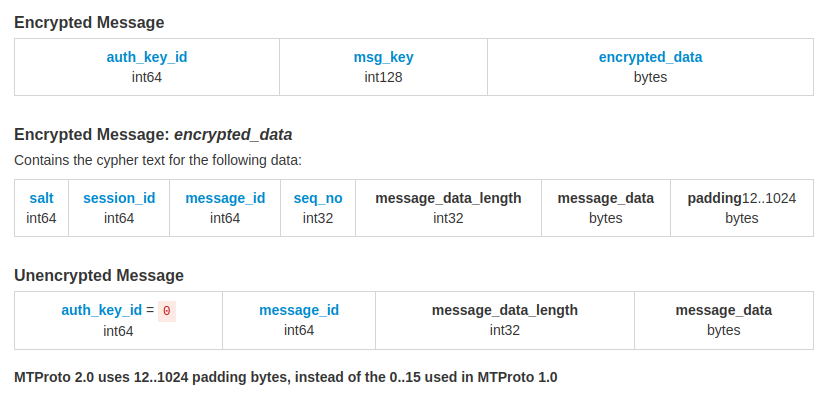
\includegraphics[scale=0.45]{imagenes/MTProto2.png} 
	\caption{Mensajes de MTProto \cite{WebProto}.}
	\label{mtproto1}
\end{figure}

\subsection{Creación de la \emph{Authorization Key}}
Como hemos visto en el apartado anterior la \emph{Authorization Key} se genera durante el registro del usuario en la aplicación. El formato de las consultas usa \emph{Binary Data Serialization}, que es un proceso en el cual se convierten los datos en binario, ya que MTProto requiere que los tipos de datos estén en formato binario y \emph{TL Language} que es un lenguaje de tipos usado para describir constructores, tipos y funciones existentes.

Los números de gran tamaño son transmitidos como cadenas que contienen la secuencias de bytes en formato \emph{big endian}, los números de menor tamaño como pueden ser los \emph{int, long int128...} usan normalmente el formato \emph{little endian}. Si pertenecen al hash generado con \emph{SHA-1} los bytes no son reorganizados.

Una vez introducidos los formatos que seguirán las consultas y los números veamos los pasos que se siguen en la creación de la \emph{Authorization Key}.

\begin{enumerate}
	\item El cliente envía una consulta al servidor, en esta consulta irá el \emph{nonce} que es un número aleatorio \emph{int128} generado por el cliente que servirá para para que el servidor lo identifique, este número no es secreto y a partir de ese momento irá incorporado en todas las consultas. Con este paso empieza el intercambio de claves \emph{Diffie-Hellman}.
	
	\item El servidor le responde enviando 
	\begin{itemize}
		\item \emph{server\_nonce}: Es un número aleatorio \emph{int128} generado por el servidor que sirve para que el cliente lo identifique y al igual que el \emph{nonce} no será secreto e irá incluido en las siguientes consultas y respuestas. 
		\item \emph{pq}: Es una representación de un número natural en formato \emph{big endian} que es el producto de dos números primos, \emph{pq} por lo general verifica $pq \leq 2^{63}-1$
		\item \emph{server\_public\_key\_fingerprints}: Es una lista de \emph{fingerprints}, secuencias únicas de letras y números usadas para identificar las claves RSA públicas.
	\end{itemize}

	\item El cliente descompone \emph{pq} en factores primos tal que $p$\textless$q$. Una vez hecho esto empieza el intercambio de claves Diffie-Hellman. Este paso es la prueba de trabajo.

	\item En este paso se presentan las pruebas de trabajo. Para ello se genera \emph{encrypted\_data} como sigue.
	\begin{enumerate}
		\item Se genera \emph{new\_nonce} un número aleatorio generado por el cliente.
		\item Se genera \emph{data} que es una serialización de:
		\begin{itemize}
			\item \emph{pq},
			\item \emph{p},
			\item \emph{q},
			\item \emph{server\_nonce},
			\item \emph{new\_nonce},
			\item \emph{dc}, que es la id del servidor con el que se está haciendo el intercambio de claves.
		\end{itemize}
		\item Se genera \emph{encrypted\_data} como el resultado de la función $RSA\_PAD(data, server\_public\_key)$. Esta es una variación de RSA cuyo funcionamiento es el siguiente.
		\begin{itemize}
			\item Se genera \emph{data\_with\_padding:=data+random\_padding\_bytes}, donde \emph{random\_padding\_bytes} se escoge de manera que \emph{data\_with\_padding} tenga un tamaño final de 192 bytes.
			\item Luego se crea la variable \emph{data\_pad\_reversed} como resultado de la función $BYTE\_REVERSE(data\_with\_padding)$, función la cual revierte el orden de los bytes.
			\item Se genera un número aleatorio de 32 bytes que se denomina como \emph{temp\_key}.
	\item Se genera $data\_with\_hash:=data\_pad\_reversed + \\ + SHA256(temp\_key + data\_with\_padding)$. Después de esta operación \emph{data\_with\_hash} tiene exactamente una longitud de 224 bytes.
	\item Después de este paso se encripta \emph{data\_with\_hash} a partir de \emph{temp\_key} usando AES-256 y se almacena el resultado en la variable \emph{aes\_encrypted}.
	\item Se ajusta \emph{aes\_encrypted} a 32 bytes usando la función SHA-256 y a continuación se realiza la operación XOR con \emph{temp\_key} almacenándose el resultado en \emph{temp\_key\_xor}.
	\item Se combinan \emph{temp\_key\_xor} con \emph{aes\_encrypted} y se almacena el resultado en \emph{key\_aes\_encrypted}. Esta tiene un tamaño de 256 bytes. 
	\item Se compara el tamaño \emph{key\_aes\_encrypted} con \emph{RSA-modulus} de \emph{server\_pub\_key} en formato big endian de 2048 bits. Si \emph{key\_aes\_encrypted} es mayor que \emph{RSA-modulus}, se empieza de nuevo el proceso eligiendo un nuevo \emph{random\_temp\_key}.
	\item Por último se genera \emph{encrypted\_data} como resultado de aplicar RSA a \emph{key\_aes\_encrypted} y a \emph{server\_pub\_key}.
		\end{itemize}
	\end{enumerate}
	Una vez hecho esto, se envía \emph{encrypted\_data} al servidor.
	Después de este paso alguien podría interceptar la consulta y modificarla con una cosulta suya haciendo un ataque \textbf{man-in-the-middle}. 
	Este ataque no sería muy efectivo, ya que el único elemento que podría modificar sería \emph{new\_nonce} porque los demás están cifrados y el resultado sería que el atacante genere una \emph{Authorization\_key} propia independiente de la del cliente haciendo que el ataque no sea efectivo.

	\item El servidor responde enviando
		\begin{itemize}
			\item \emph{nonce}.
			\item \emph{server\_nonce}.
			\item \emph{encrypted\_answer}: Respuesta cifrada que es del tipo \emph{string} y a su vez contiene
			\begin{itemize}
				\item \emph{new\_nonce\_hash}: Son los 128 bits menos significativos de \emph{SHA-1(new\_nonce)}.
				\item \emph{answer}: Es una serialización de \emph{nonce}, \emph{server\_nonce}, \emph{g}, \emph{dh\_prime}, \emph{g\_a} y \emph{server\_time}. Donde \emph{dh\_prime} es un número primo seguro de 2048 bits, \emph{g} un generador de un subgrupo cíclico de orden $\frac{p-1}{2}$, $g_a$ es la clave que envía el servidor al cliente que al elevarla a $b$ módulo \emph{dh\_prime} el cliente obtendría la clave final.
\item \emph{answer\_with\_hash}: Es una generación con la función hash \emph{HASH1} quedando como \emph{SHA-1(answer)}+\emph{answer}+\emph{(0-15 bytes aleatorios)} de manera que la longitud sea divisible por 16, es del tipo \emph{string}.
				\item \emph{answer\_aes\_key}: \emph{SHA-1(new\_nonce + server\_nonce) +\\+ substr(SHA-1(server\_nonce + new\_nonce), 0, 12)} y es del tipo \emph{string}. Donde \emph{substr} es una función que devuelve caracteres del \emph{string} desde una posición hasta otra, en este caso desde la posición $0$ hasta $12$.
				\item \emph{tmp\_aes\_iv}: \emph{substr(SHA-1(server\_nonce + new\_nonce), 12, 8) + SHA-1(new\_nonce + new\_nonce) + substr(new\_nonce, 0, 4)}
				\item \emph{encrypted\_answer}: \emph{AES256\_ige\_encrypt(answer\_with\_hash,\\ tmp\_aes\_key, tmp\_aes\_iv)} donde:
				\begin{itemize}
					\item \emph{tmp\_aes\_key}: Es una clave de 256 bits
					\item \emph{tmp\_aes\_iv}: Es un vector de inicialización de 256 bits.
				\end{itemize}
				Al igual que en el resto de las instancias que usan el cifrado AES, a los datos cifrados se le añaden bytes aleatorios de forma que el tamaño sea divisible por 16.
			\end{itemize}
		\end{itemize}
	Después de este paso \emph{new\_nonce} sigue siendo únicamente conocido por el cliente y el servidor de esta manera el cliente garantiza que el servidor es el que está al otro lado de la comunicación y que la respuesta de este es correcta, ya que los datos están cifrados usando \emph{new\_nonce}.

	El cliente comprueba que $p=dh\_prime$, es un número primo seguro de 2048 bits, es decir, se tiene que verificar que \emph{p} y $\frac{p-1}{2}$ son primos, además, $2^{2047}$\textless \emph{p} \textless $2^{2048}$, y \emph{g} genera un subgrupo cíclico con orden primo $\frac{p-1}{2}$.$g$ siempre vale 2, 3, 4, 5, 6, o 7.

	Si la verificación tarda mucho tiempo, cosa que ocurre en dispositivos antiguos, se ejecutarían solo 15 iteraciones en el algoritmo de Miller-Rabin para garantizar que \emph{p} y $\frac{p-1}{2}$ sean primos con una probabilidad de error muy baja, alrededor de una millonésima, y dejar el resto de iteraciones para después, ejecutándose estas de fondo.

	\item El cliente genera un número aleatorio \emph{b} de 2048 bits y lo envía al servidor en un mensaje que contiene:
		\begin{itemize}
			\item \emph{nonce}.
			\item \emph{server\_nonce}.
			\item \emph{encrypted\_data} que se descifra de la siguiente manera:
				\begin{itemize}
					\item \emph{g\_b} = $g^b$ mod \emph{dh\_prime}
					\item \emph{data} que es una serialización donde
						\begin{itemize}
							\item \emph{nonce}
							\item \emph{server\_nonce}
							\item \emph{retry\_id} que vale 0 en el primer intento y en caso contrario, vale \emph{auth\_key\_aux\_hash} del intento fallido anterior y es del tipo \emph{long}.
							\item \emph{g\_b} que es del tipo \emph{string}.
						\end{itemize}
					\item \emph{data\_with\_hash} que es: \emph{SHA-1(data)+data+(0-15 bytes aleatorios de manera que el tamaño sea divisible por 16)}.
					\item \emph{encrypted\_data} que es: \emph{AES256\_ige\_encrypt(data\_with\_hash, tmp\_aes\_key, tmp\_aes\_iv)}. Donde el modo IGE es una variación de modo CBC [\ref{esquemacbc}] de los cifrados de bloque. En este modo se garantiza que si un bloque del mensaje encriptado es cambiado, no se pueda desencriptar correctamente el mensaje completo.
				\end{itemize}
		\end{itemize}
	\item Una vez hecho los pasos previos tendríamos que \emph{auth\_key} vale $g^{ab}$ mod \emph{dh\_prime}, en el servidor se calcula como \emph{$g\_b^{a}$ mod \emph{dh\_prime}} y en el cliente se calcula como $g\_a^b$ mod \emph{dh\_prime}.
	\item \emph{auth\_key\_hash} se calcula como los 64 bits de menor prioridad de \emph{SHA-1(auth\_key)}. El servidor comprueba si existe alguna otra clave con el mismo \emph{auth\_hash} y responde de alguna de las siguientes tres formas
	\begin{enumerate}
		\item Una serialización de: 
			\begin{itemize}
				\item \emph{nonce},
				\item \emph{server\_nonce},
				\item \emph{new\_nonce\_hash1}.
			\end{itemize}
		\item Una serialización de:
			\begin{itemize}
				\item \emph{nonce},	
				\item \emph{server\_nonce},
				\item \emph{new\_nonce\_hash2}.
			\end{itemize}
		\item Una serialización de:
			\begin{itemize}
				\item \emph{nonce},	
				\item \emph{server\_nonce},
				\item \emph{new\_nonce\_hash3}.
			\end{itemize}
	\end{enumerate}
	Donde \emph{new\_nonce\_hash1}, \emph{new\_nonce\_hash2} y \emph{new\_nonce\_hash3} son los 128 bits menos significativos de SHA-1 de la cadena de bytes obtenida al añadir a \emph{new\_nonce} un byte con el valor 1,2 o 3 respectivamente y seguido de \emph{auth\_key\_hash}.

	\emph{Auth\_key\_aux\_hash} son los 64 bits más significativos del resultado de la función hash \emph{SHA-1(auth\_key)}.

	Si algo falla durante estos pasos, el cliente volvería al paso 6 y generándose un nuevo \emph{b}. Al mismo tiempo se define \emph{server\_salt} como \emph{substr(new\_nonce, 0, 8)} XOR \emph{substr(server\_nonce, 0, 8)}.
\end{enumerate}
\textbf{Gestión de errores}

Si el cliente no obtiene alguna respuesta del servidor en un intervalo de tiempo determinado se repite la consulta, análogamente ocurre con el servidor. Sin embargo si el servidor no obtiene una segunda respuesta del cliente en 10 minutos, reiniciará la conexión y el cliente tendrá que empezar de nuevo.

\subsection{Generando la clave y el vector de inicialización de AES}
En esta sección hablaré de como se generan la clave de autorización (\emph{auth\_key}) y de la clave del mensaje (\emph{msg\_key}) necesarias para calcular la clave de AES (\emph{aes\_key}) y el vector de inicialización de 256 bits (\emph{iv\_aes}) usados para cifrar los mensajes en MTProto 2.0.\\
El algoritmo sigue los siguientes pasos.
\begin{enumerate}
	\item Calculamos \emph{msg\_key\_large} como \emph{SHA-256(substr(auth\_key, 88+x, 32)+plaintext+random\_padding)}.
	\item Calculamos \emph{msg\_key} como \emph{substr(msg\_key\_large, 8, 16)}.
	\item Calculamos \emph{sha256\_a} como \emph{SHA-256(msg\_key+substr(auth\_key, x, 36))}.
	\item Calculamos \emph{sha256\_b} como \emph{SHA-256(substr(auth\_key, 40+x,\\ 36)+msg\_key)}.
\end{enumerate}
Y una vez hechos estos pasos, ya podemos calcular la clave para AES y el vector de inicialización.
\begin{itemize}
	\item \textbf{\emph{aes\_key}}: \emph{substr(sha256\_a, 0, 8)+substr(sha256\_b, 8, 16)+\\+substr(sha256\_a, 24, 8)}.
	\item \textbf{\emph{aes\_iv}}: \emph{substr(sha256\_b, 0, 8) + substr(sha256\_a, 8 16)+\\+substr(sha256\_b, 24, 8)}.
\end{itemize}
\emph{x} vale 0 cuando los mensajes van del cliente al servidor y 8 cuando los mensajes van del servidor al cliente.\\
Los 1024 bits menos significativos de la \emph{auth\_key} no se utilizan para el cálculo ya que estos se usan para cifrar la copia local de los datos recibidos del servidor además, los 512 bits menos significativos no se almacenan en el servidor por lo que si el cliente pierde la clave o la contraseña del dispositivo, no se podrán descifrar los datos locales. Un esquema del proceso se puede ver en \ref{mtproto2}.
%\newpage
\begin{figure}[htb]
	\centering
	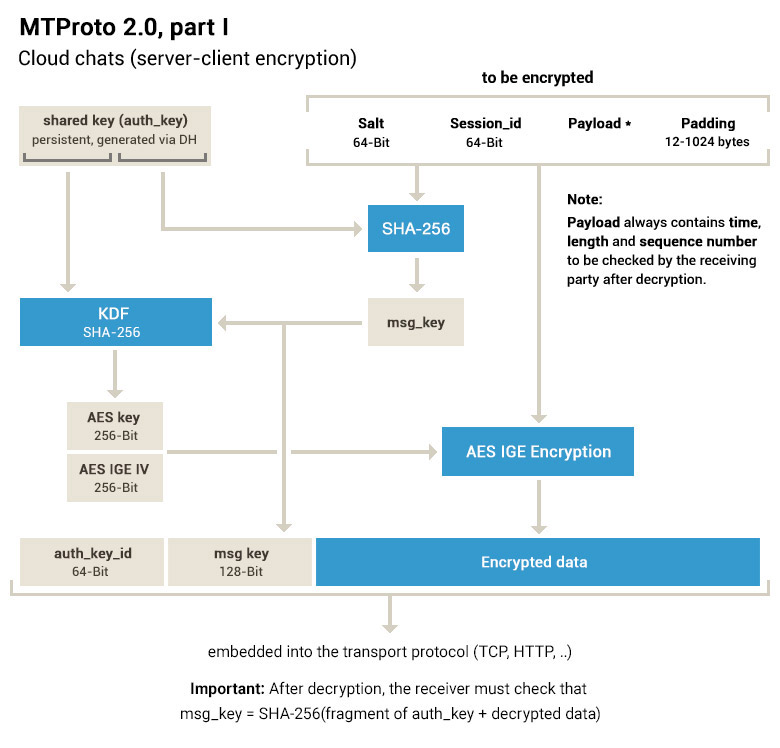
\includegraphics[scale=0.4]{imagenes/diagramaMTProto.jpg} 
	\caption{Esquema del cifrado de mensajes usado en MTProto 2.0 \cite{WebProto}.}
	\label{mtproto2}
\end{figure}

\subsection{Envío de mensajes}
Una vez realizado el intercambio de claves mediante \emph{Diffie-Hellman} y la generación de la clave y el vector de inicialización de AES ya se podrían enviar mensajes cifrados entre el cliente y el servidor utilizando \emph{AES256}.
Los protocolos de transporte que están disponibles son los siguientes.
\begin{itemize}
	\item \emph{TCP}
	\item \emph{WebSocket}
	\item \emph{WebSocket} sobre \emph{HTTPS}
	\item \emph{HTTP}
	\item \emph{HTTPS}
	\item \emph{UDP}
\end{itemize}


\section{WhatsApp, Facebook Menssenger y Signal (TextSecure Protocol)}
El protocolo \emph{TextSecure Protocol} también conocido como \emph{Signal} fue desarrollado por Trevor Perrin y Moxie Marilinspike que trabajaban en la empresa Open Whisper Systems en 2013. Se implementó inicialmente en la aplicación de mensajería homónima \emph{Signal} aunque posteriormente se introdujo en otras aplicaciones de mensajería como \emph{WhatsApp} y \emph{Facebook Menssenger}.

Este protocolo ha tenido 3 versiones.
\begin{itemize}
	\item \textbf{TextSecure v1.} Es la primera versión del protocolo, que fue lanzada en 2013 y estaba basada en el protocolo \emph{Off-the-Record Messaging (OTR)}.
	\item \textbf{TextSecure v2.} Es la segunda versión publicada el 24 de febrero de 2014. Esta versión extendió el protocolo con \emph{Double Ratchet Algorithm} el cual un intercambio de claves \emph{Diffie-Hellman} con una \emph{función de derivación de clave (KDF)} usando funciones hash, permitiendo extender las claves y aumentando la seguridad del protocolo.
	\item \textbf{TextSecure v3.} Esta tercera versión fue lanzada en octubre de 2014 y añadió algunos cambios a las primitivas criptográficas y al protocolo de red.
\end{itemize}
Cabe a mencionar que aunque el protocolo originalmente el protocolo se llamaba \emph{TextSecure} en 2016 fue renombrado como \emph{Signal Protocol} que es como lo conocemos hoy en día.

La información técnica de este protocolo que voy a desarrollar a continuación ha sido obtenida de \cite{November2021b}.

\subsection{Descripción general y dispositivos}
El protocolo \emph{Signal} es un protocolo diseñado para prevenir que aplicaciones como \emph{WhatsApp, Signal y Facebook Messenger} sean vulneradas de manera que se pueda acceder a la información intercambiada en los mensajes y las llamadas. Este protocolo permite que un usuario tener diversos dispositivos cada uno con su propias claves garantizando que si se obtiene alguna de ellas, los mensajes enviados por alguno de los otros dispositivos no puedan ser descifrados. Además también es usado en el caso de \emph{WhatsApp} para cifrar el historial de mensajes y enviarlo a un nuevo dispositivo del mismo usuario.

Por comodidad voy a explicar el protocolo para WhatsApp dado que para el resto de aplicaciones que lo usan hacen un uso igual de este.

\subsubsection{Tipo de dispositivos}
Como he me mencionado anteriormente, el protocolo \emph{Signal} permite tener varios dispositivos asociados al usuario, si bien no todos los dispositivo son iguales. Se pueden distinguir dos tipos de dispositivos.
\begin{itemize}
	\item \textbf{Dispositivo principal.} Dispositivo único utilizado para vincular una cuenta de \emph{WhatsApp} con un número de teléfono. Este dispositivo permite vincular dispositivos adicionales que serán los dispositivos compañeros.
	\item \textbf{Dispositivo Compañero o Secundario.} Es un dispositivo vinculado a una cuenta existente de WhatsApp, a diferencia del dispositivo principal, este no tiene porque ser único.
\end{itemize}
Ciertas aplicaciones únicamente pueden ser usadas en dispositivos principales como pueden ser las aplicaciones para \emph{Android} y \emph{iOS}.

\subsection{Descripción de las claves}
En este apartado hablaré acerca de las distintas claves que se utilizan para cifrar y descifrar los datos.
\begin{itemize}
	\item \textbf{Claves públicas}
		\begin{itemize}
			\item \emph{Identity Key Pair}: Es un par de claves de largo plazo del tipo \emph{Curve25519} generadas en la instalación.
			\item \emph{Signed Pre Key}: Es una clave de medio plazo del tipo \emph{Curve25519} generada durante la instalación y firmada por la \emp{Identity Key} que se va rotando de manera periódica a lo largo del tiempo.
			\item \emph{One-Time Pre Keys}: Es un lote de pares de claves del tipo \emph{Curve25519} de un solo uso generadas en la instalación y siendo posible volver a generarlas en caso de ser necesario.
		\end{itemize}
	\item \textbf{Claves de Sesión}
		\begin{itemize}
			\item \emph{Root Key}: Clave de 32 bytes usada para generar \emph{Chain Key}.
			\item \emph{Chain Key}: Clave de 32 bytes usada para generar \emph{Message Key}.
			\item \emph{Message Key}: Clave de 80 bytes usada para cifrar los mensajes. Están formadas por 32 bytes usados para la clave \emph{AES256}, 32 bytes para la clave \emph{HMAC-SHA256} y 16 bytes para un \emph{IV}.
		\end{itemize}
	\item \textbf{Otras claves}
		\begin{itemize}
			\item \emph{Linking Secret Key}: Es una clave de 32 bytes generada en un \emph{dispositivo compañero} y que tiene que ser enviada por un canal seguro al \emph{dispositivo principal}. Se usa para verificar un \emph{HMAC} del intercambio durante la vinculación entre los dispositivos. Se envía escaneando un código QR.
		\end{itemize}
\end{itemize}

\subsection{Otros elementos relacionados con los dispositivos compañeros}
\begin{itemize}
	\item \emph{Linking Metadata}: cifrado de metadatos asignados a un dispositivo compañero durante la etapa de vinculación, se usa a la par que la \emph{Identity Key} para identificar un dispositivo compañero entre los dispositivos de WhatsApp.
	\item \emph{Signed Device List Data}: Lista cifrada que identifica los dispositivos compañeros vinculados a la cuenta principal en el momento de la firma. Se firma con la \emph{Identity Key} del dispositivo principal usando 0x0602 como prefijo.
	\item \emph{Account Signature}: Firma del tipo \emph{Curve25519} calculada a partir del prefijo 0x600, \emph{Linking Metadata} y la \emph{Identity Key} del dispositivo compañero usando la \emph{Identity Key} del dispositivo principal.
	\item \emph{Device Signature}: Firma del tipo \emph{Curve25519} calculada a partir del prefijo 0x601, \emph{Linking Metadata}, la \emph{Identity Key} del dispositivo compañero y la \emph{Identity Key} del dispositivo principal usando la \emph{Identity Key} del dispositivo compañero. 
\end{itemize}

Una vez introducido la terminología que se va a usar el la descripción del protocolo \emph{Signal}, procederé a describir las etapas principales de este.\\

\subsection{Registro de clientes}
Etapa inicial consistente en añadir dispositivos asociados al cliente, como se ha visto anteriormente existen dos tipos de dispositivos: \emph{dispositivo principal} y \emph{dispositivos compañeros} y en función del tipo se registrarán de manera diferente.
\begin{description}
	\item \textbf{Dispositivo principal}\\
	Durante el momento del registro, el cliente de WhatsApp envía al servidor su \emph{Identity Key}, su \emph{Signed Pre Key} con una firma y conjunto de \emph{One-Time Pre Keys}. Una vez enviadas el servidor de WhatsApp almacena estas estas claves públicas asociadas con el identificador del usuario.

	\item \textbf{Dispositivo compañero}\\
	Para vincular un nuevo dispositivo a la cuenta de WhatsApp, el dispositivo principal del usuario crea al principio una firma de la cuenta firmando la \emph{Identity Key} del nuevo dispositivo, a su vez, el dispositivo compañero que se quiere introducir firmando la \emph{Identity Key} pública del dispositivo principal. Una vez que se han realizado ambas firmas, ya se puede iniciar las sesión con el dispositivo compañero usando un cifrado \emph{end-to-end}.\\Los pasos seguidos son:
	\begin{enumerate}
		\item El dispositivo muestra su \emph{Identity Key} ($I_{companion}$) y genera un una clave temporal para vincularse ($L_{companion}$) en un código QR. Esta clave nunca será enviada al servidor.
		\item El dispositivo principal escanea el código QR y almacena $I_{companion}$ en el disco.
		\item El dispositivo principal carga su propia \emph{Identity Key} como $I_{primary}$.
		\item El dispositivo genera los metadatos de la vinculación ($L_{metadata}$) y actualiza la lista de datos de dispositivos para que contenga un nuevo dispositivo compañero como ($L_{istData}$).
		\item El dispositivo principal genera una firma de la cuenta para el compañero, $$A_{signature}=CURVE25519\_SIGN(I_{primary} || L_{metadata} || I_{companion}).$$
		\item El dispositivo principal genera una firma para la lista de dispositivos que permitirá actualizar la propia lista de dispositivos. $$ListSignature = CURVE25519\_SIGN(I_{primary}, 0x0602 || ListData).$$
		\item El dispositivo principal agrupa los datos de la vinculación en $L_{data}$, conteniendo este $L_{metadata}$, $I_{primary}$ y $A_{signature}$.
		\item El dispositivo principal genera una \emph{HMAC} para la vinculación y\\ una \emph{PHMAC} que será igual a $HMAC-SHA256(L_{companion}\\, L_{data})$. Una vez hecho esto enviará \emph{ListData}, \emph{ListSignature}, $L_{data}$ y la \emph{PHMAC} al servidor.
		\item El servidor almacena \emph{ListData} y \emph{ListSignature} y reenvía $L_{data}$ y la \emph{PHMAC} al dispositivo compañero.
		\item El dispositivo compañero  verfica la \emph{PHMAC}, decodifica \emph{Ldata} en \emph{Lmetadata}, \emph{Iprimary} y \emph{Asignature} verificando esta última.
		\item El dispositivo compañero almacena $L_{metadata}$ e $I_{primary}$ en el disco.
		\item A continuación este genera una firma del dispositivo por si mismo que es de la forma\\ 
		\begin{aligned}
			D_{signature}=CURVE25519\_SIGN(I_{companion}, 0x0601 || \\ || L_{metadata} || I_{companion} || I_{primary}).
		\end{aligned}
		\item El dispositivo compañero sube al servidor de WhatsApp: $L_{metadata}$, $A_{signature}$, $D_{signature}$, $I_{companion}$, la \emph{Signed Pre Key} pública del dispositivo firmada y un lote de \emph{Pre Keys} de un solo uso.
		\item El servidor almacena los datos subidos asociados con la identificación del usuario combinados con el identificador especifico del dispositivo.
	\end{enumerate}
\end{description}


\begin{figure}[htb]
	\centering
	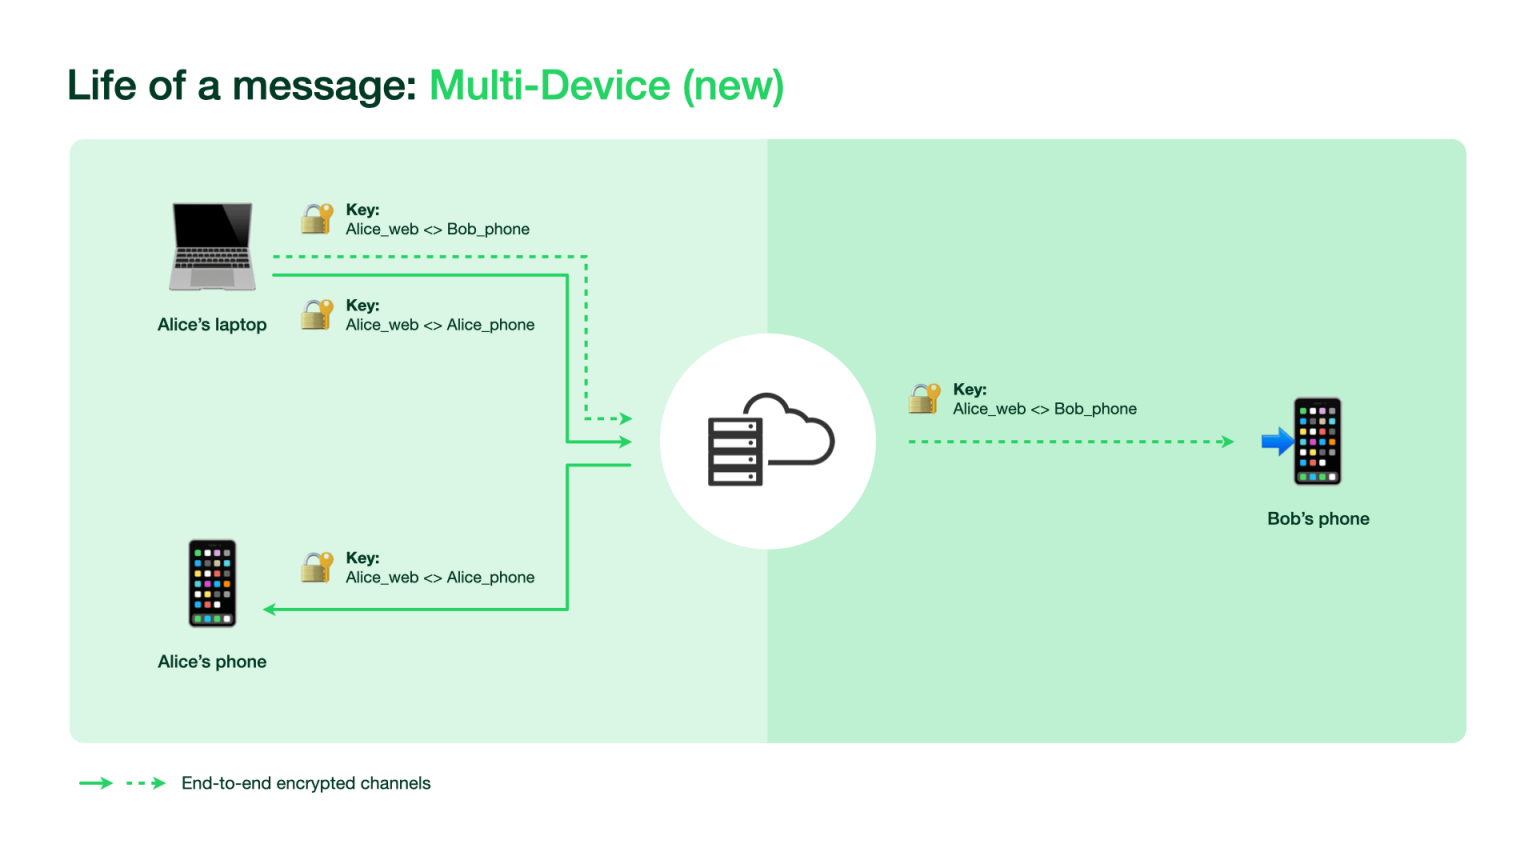
\includegraphics[scale=0.25]{imagenes/what1.png} 
	\caption{Diagrama de un conexión entre dos dispositivos teniendo uno de ellos un dispositivo compañero \cite{what1}.}
	\label{what1}
\end{figure}

\subsection{Inicio de sesión}
Para que la comunicación entre usuarios sea segura y privada el emisor establece una conexión por pares con cada uno de los dispositivos del receptor. Una vez que la conexión entre emisor y receptor ha sido establecida, no es necesario volver a establecerla a no ser que la sesión se pierda.

Lo pasos que se siguen para establecer una conexión son los siguientes.
\begin{enumerate}
	\item El cliente que inicia la conexión solicita la \emph{identity key}, la \emph{Signed Pre key} y un lote de \emph{Pre keys} de un solo uso para cada dispositivo del receptor y los dispositivos adicionales que el mismo posee excluyendo el dispositivo desde el que se inicia la conexión. 
	\item El servidor devuelve todo lo solicitado y elimina las \emph{Pre keys} enviadas ya que son de un solo uso. Sí el último lote de \emph{Pre keys} enviado es agotado y el receptor no los ha repuesto no se devuelve ninguna clave. Además, por cada dispositivo compañero que haya tanto del emisor como del receptor, el servidor devuelve $L_{metadata}$, $A_{signature}$ y $D_{signature}$ que fueron enviadas por el dispositivo compañero cuando se vinculó.
	\item Por cada conjunto de claves devueltas, el emisor tiene que verificar \emph{Asignature} con\\ $CURVE25519\_VERIFY \_SIGNATURE(I_{primary}, 0x0600 || L_{metadata}\\ || I_{companion})$.\\
	$D_{signature}$ es obtenida con\\ $CURVE25519\_VERIFY\_SIGNATURE(I_{companion},0x0601 ||\\ L_{metadata} || I_{companion} || I_{primary})$.
	Si en algún momento la verificación falla, el emisor termina la sesión de cifrado y no envía ningún mensaje al dispositivo que ha fallado.
\end{enumerate}
Una vez obtenidas las claves del servidor y se ha verificado la identidad, el emisor inicia la sesión de encriptación con cada dispositivo individualmente. Para ello se siguen los siguientes pasos:
\begin{enumerate}
	\item El emisor almacena la \emph{Identity Key} del receptor como $I_{recipient}$, la \emph{Signed Pre Key} como $S_{recipient}$ y la \emph{Pre Key} de un solo uso como $O_{recipient}$.
	\item El emisor genera un par de pares de claves efímeras \emph{Curve25519} llamada $E_{initiator}$.
	\item El emisor carga su propia \emph{Identity Key} como $I_{initiator}$.
	\item El emisor calcula el \emph{master\_secret} como \\
	\begin{aligned}
			master\_secret = ECDH(I_{initiator}, S_{recipient}) || ECDH(E_{initiator}, I_{recipient})||\\ || ECDH(E_{initiator}, S_{recipient}) || ECDH(E_{initiator}, O_{recipient}). &
	\end{aligned}
	Cabe a mencionar que \emph{ECDH} es el intercambio de claves \emph{Diffie-Hellman}.
	\item El emisor usa \emph{HKDF} para crear una \emph{Root Key} y una \emph{Chain Key} de \emph{master\_secret}. Donde HKDF es una función de derivación de claves simple basada en el código de autenticación de mensajes \emph{HMAC}\cite{cekd}.
\end{enumerate}

\subsection{Intercambio de mensajes}
Una vez que la sesión se ha establecido, los clientes intercambian los mensajes encriptados con \emph{Message Key} usando \emph{AES-256} con el modo \emph{CBC}[\ref{esquemacbc}] y para la autenticación \emph{HMAC-SHA256}. \emph{Message Key} cambia con cada mensaje que se envía y además es efímera para que esta no pueda ser reconstruida una vez que el mensaje sea transmitido y recibido. Esta clave se obtiene a partir de la \emph{Chain Key} del receptor que se regenera con cada intercambio de mensajes. 

\subsection{Cálculo de \emph{Message Key} a partir de \emph{Chain Key}}
La \emph{Message Key} se genera:
\begin{enumerate}
	\item $Message Key = HMAC$-$SHA256(Chain Key, 0x01)$.
	\item La \emph{Chain Key} es actualizada como \\ $Chain Key = HMAC$-$SHA256(Chain Key, 0x02)$.
\end{enumerate}
Este último paso hace que la \emph{Chain key} cambie haciendo imposible que con una \emp{Message Key} antigua se obtenga la \emph{Chain Key} actual.

\subsection{Cálculo de \emph{Chain Key} a partir de \emph{Root Key}}
Cada vez que un mensaje es enviada una clave pública efímera \emph{Curve25519}. Una vez que la respuesta es definida se calcula una nueva \emph{Chain Key} y una nueva \emph{Root Key} de la siguiente forma:
\begin{enumerate}
	\item $ephemeral$\_$secret = ECDH(Ephemeral_{sender}, Ephemeral_{recipient})$.
	\item $Chain$ $Key$, $Root$ $Key$ $= HKDF(Root$ $Key, ephemeral$\textunderscore$secret)$.
\end{enumerate}

\section{iMessage}
iMessage es una aplicación de mensajería diseñada para ser utilizada en dispositivos iOS, iPadOS, Apple Watch y ordenadores con MacOS. Esta aplicación permite enviar mensajes de texto, y archivos como pueden ser fotos, contactos, ubicaciones etc. La información para este apartado ha sido obtenido mayormente de \cite{apple2} y \cite{apple1}.\\

\subsubsection{Funcionamiento criptográfico}
Para iniciar una nueva conversación a partir de una dirección o un nombre. En caso de usar un número de teléfono o una dirección de correo electrónico, la aplicación contacta con el servicio de identidad de Apple (\emph{IDS}). Este es un directorio de claves públicas de iMessage, direcciones del servicio de notificaciones push de Apple (APNs), números de teléfono y direcciones de correo electrónico usadas para obtener las claves y direcciones de los dispositivos \cite{ids}. Una vez que se pone en contacto con este se obtienen las claves públicas y las direcciones APNs de todos los dispositivos asociados al destinatario.

Una vez obtenidas las claves, el mensaje que se envía es encriptado de manera individual para cada uno de los dispositivos del destinatario. Tanto las claves públicas usadas como las clases de firmas se obtienen del IDS. El emisor genera un valor aleatorio de 88bits para cada dispositivo de destino del destinatario y este es utilizado como clave \emph{HMAC-SHA256} para crear una valor de 40 bits a partir de la clave pública del emisor, receptor y del texto sin formato. Los 88 bits generados aleatoriamente se combinan con los 40 bits obtenidos para formar una clave de 128 bits para encriptar el mensaje usando el estándar AES en modo contador (CTR).
El dispositivo receptor usa el valor de 40 bits para comprobar la integridad del texto sin formato una vez que este es desencriptado.

Para encriptar esta clave AES se usa REA-OAEP para la clave pública con el dispositivo receptor. Una vez encriptados el mensaje y la clave se genera un hash SHA1 el cual es firmado con el algoritmo de firma digital de curva elíptica ECDSA, para esto también se usa la clave de firma privada del emisor. En dispositivos más recientes que tengan un sistema operativo iOS13 o posterior y iPadOS 13.1 o posterior se puede utilizar ECIES en lugar de RSA.

Los mensajes obtenidos después del proceso encriptación contienen:
\begin{itemize}
	\item Texto del mensaje encriptado.
	\item Clave del mensaje encriptada.
	\item Firma digital del emisor.
\end{itemize}
Para enviar los mensajes se mandan al APNs, donde los metadatos asociados a este como son la fecha o la información sobre el enrutamiento del APNs no son encriptados. Para comunicarse con el APNs se una comunicación encriptada a través de un canal TLS de secreto-hacia-delante.

Como el APNs solo puede emitir mensajes de 4 o 16KB como máximo dependiendo de la versión del sistema operativo. Por lo que si el mensaje tiene un tamaño más grande como podría pasar si se envía una foto o un vídeo, lo que se hace es encriptar el archivo adjunto con AES en modo CTR utilizando una clave de 256 bits generada aleatoriamente y se carga en iCloud. Una vez subido el archivo encriptado se envía al receptor la clave AES del archivo adjunto, su identificador uniforme de recursos(URI) y un hash SHA1 de su forma encriptada.

En el siguiente esquema se puede ver resumido el proceso de encriptado y desencriptado de los mensajes.
\begin{figure}[htb]
	\centering
	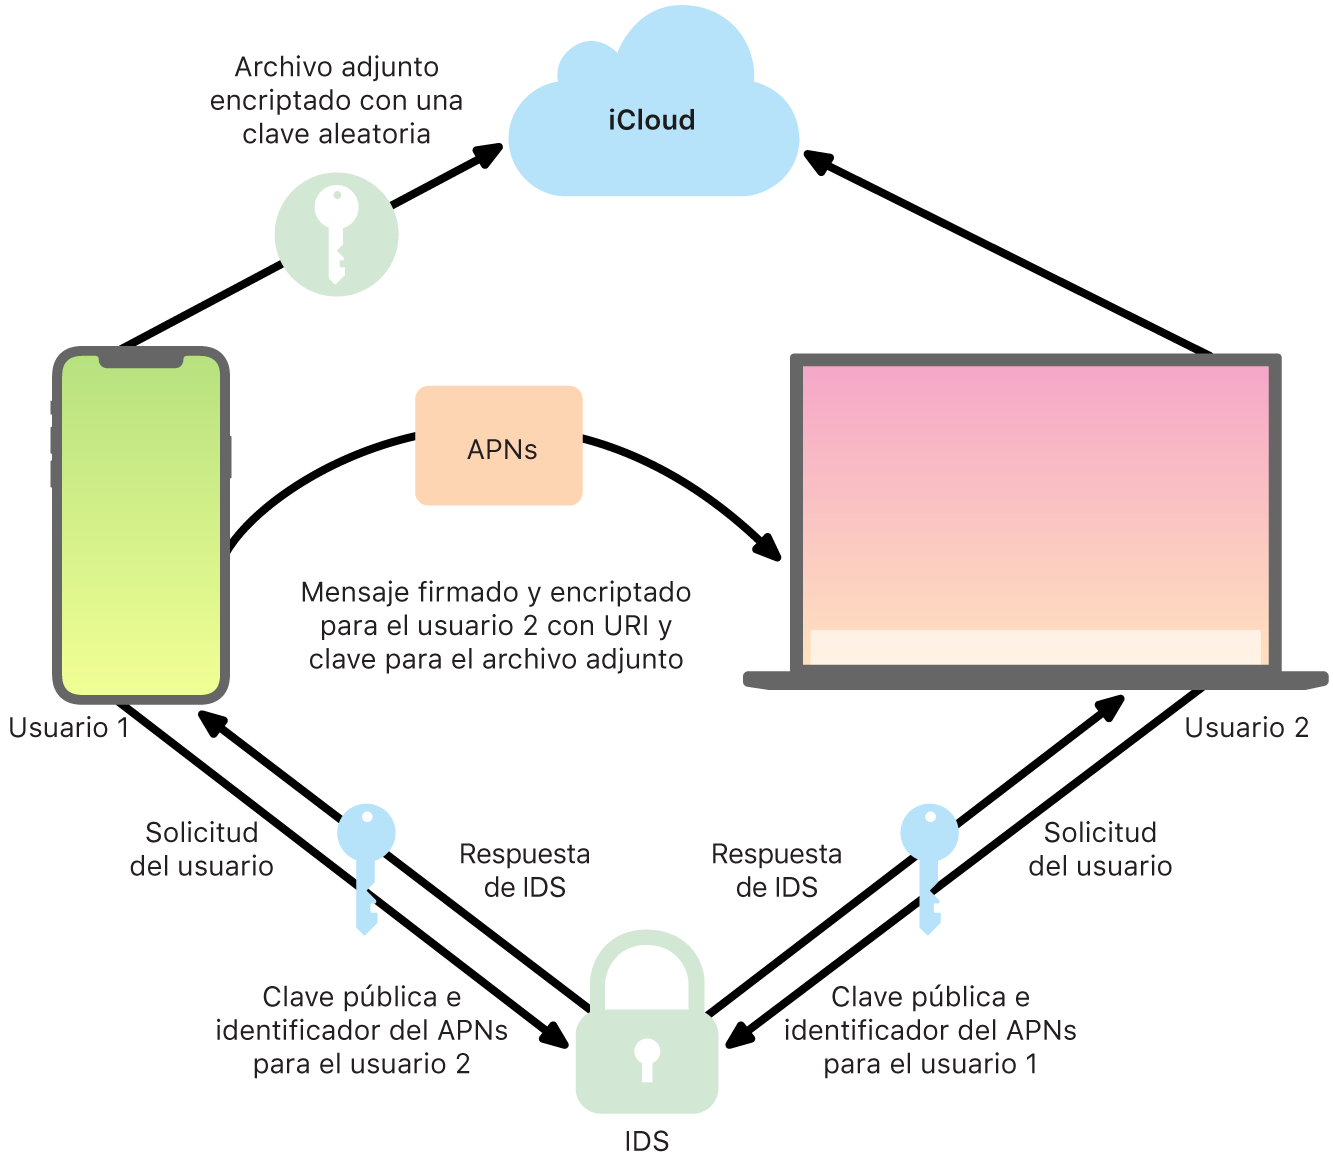
\includegraphics[scale=0.15]{imagenes/apple.png} 
	\caption{Esquema de cifrado en iMessage \cite{apple1}.}
	\label{iMessagefoto}
\end{figure}

Al igual que en las notificaciones push, los mensajes son eliminados del APNs una vez que se envían. Si es verdad que a diferencia de otras notificaciones que se envían del APNs, los mensajes se guardan en una cola para enviarlos a dispositivos sin conexión. Esto permite almacenar los mensajes en un plazo de 30 días máximo permitiendo así que un mensaje llegue tiempo después a un dispositivo que esta sin conexión.

\section{Line Messenger (Letter Sealing)}
Line es una aplicación de mensajería diseñada para ser utilizadas en dispositivos móviles y ordenadores independientemente del sistema operativo. Fue diseñada en 2011 por la empresa surcoreana NHN en Japón.
Apareció con la finalidad de paliar la caída de los servicios de telefonía en Japón debido al terremoto. Utiliza un protocolo criptográfico criptográfico propio llamado \emph{Letter Sealing}.

Este protocolo apareció en 2016 y en la actualidad cuenta con dos versiones.
\begin{itemize}
	\item \textbf{Letter Sealing v1}. Fue desarrollado en 2016 y garantiza una protección extremo a extremo en mensajes individuales y en grupo.
	\item \textbf{Letter Sealing v2}. Fue desarrollado en 2019. Gracias a un \emph{Bug Bounty  Program}, iniciativa por la cual se recompensa a las personas que descubren y notifican errores de software,  desarrollado por Takanori Isobe y Kazuhiko Minematsu se encontraron una serie de vulnerabilidades que aunque en ese momento no eran explotables, en un futuro si podrían llegar a serlo. Por ello se decidió desarrollar una nueva versión de este que garantizara una mayor seguridad.
\end{itemize}
La información para esta sección ha sido obtenida de \cite{line}.
\begin{table}[htb]
\resizebox{\textwidth}{!}{%
	\begin{tabular}{|c|cc|}
	\hline
                             & \multicolumn{1}{c|}{\textbf{v1}}                       & \textbf{v2}          \\ \hline
		Intercambio de claves       & \multicolumn{2}{c|}{ECDH sobre Curve255195}                  \\ \hline
		Algoritmo para encriptar mensajes & \multicolumn{1}{c|}{AES256-CBC}               & AES256-GCM6 \\ \hline
		Función Hash del mensaje        & \multicolumn{1}{c|}{SHA-256}                  & N/A         \\ \hline
		Autenticación de los mensajes        & \multicolumn{1}{c|}{AES-ECB con SHA-256 MAC} & AES256-GCM  \\ \hline
	\end{tabular}
	}
	\label{table:lsv}
	\caption{Tabla comparativa de versiones de Letter Sealing.}
\end{table}

\subsection{Generación de claves}
Al igual que en las aplicaciones de mensajería vistas, en \emph{Letter Sealing} se generan un par de claves por cada dispositivo del usuario. Si no existe ninguna en el dispositivo, se genera un par y se almacenan de manera segura en el almacenamiento privado de la aplicación.

Una vez generadas la clave pública se registra en un servidor de LINE, el servidor la asocia la clave al usuario de LINE y le devuelve un \emph{ID} de clave único. Este \emph{ID} representa la última versión de clave pública del usuario. 

\subsection{Intercambio de claves}
Para poder intercambiar mensajes utilizando \emph{AES-256} los usuarios tienen que intercambiar previamente una clave secreta para poder cifrar los mensajes. Para ello se utiliza el intercambio de claves \emph{Diffie-Hellman} sobre la familia de curvas \emph{curve25519} como hemos visto en el capítulo 4.

Todo el proceso es transparente para los usuarios y no se necesita de otro elemento para verificar las claves públicas. Esto se debe a que LINE permite a los usuarios ver las huellas de sus recipientes de clave pública.

\subsection{Cifrado de mensajes}
El funcionamiento de cifrado de mensajes en \emph{Letter Sealing v2} es el siguiente.
\begin{enumerate}
	\item Se deriva una clave para el cifrado usando dos valores, la clave secreta intercambiada durante el intercambio de claves (\emph{SharedSecret}) y valor aleatorio de 16 bytes generado aleatoriamente.
		$$
			salt = random_{secure}(16).
		$$
		$$
			Key_{encrypt}=SHA256(SharedSecret||salt||"Key").
		$$
	\item Se calcula \emph{nonce} concadenando 8 bytes por cada contador de chat ($per\_chat_{counter}$) con 4 bytes generados aleatoriamente.
		$$
			nonce[12]=per\_chat_{counter}[8] || random_{secure}(4).
		$$
	\item Se encripta el payload (\emph{M}) del mensaje usando \emph{AES256-GCM}, usando $Key_{encrypt}$ y $nonce$. En \emph{Letter Sealing v2} se añade unos metadatos al mensaje (\emph{AAD}) para reforzar la integridad del mensaje. Se calcula de la siguiente manera.
		$$
			ADD =
		$$
		$$
			 recipientID\:||\: senderID\:||\:senderkeyID\:||\:recipientkeyID\:||\:version\:||\:contenttype.
		$$
		También se utiliza una función llamada \emph{GCM} que es un esquema \emph{AEAD}, \emph{Authenticated Encryption with Associated Data} que garantiza la integridad y confidencialidad del mensaje. La salida del cifrado sería la siguiente.
		$$
			(C,tag) = AES - GCM(Key_{encrypt}, nonce, M, AAD).
		$$
	\item Una vez seguidos estos pasos el emisor envía al receptor un mensaje que consta de los siguientes elementos.\\
	\begin{itemize}
		\item \emph{version},
		\item \emph{content type},
		\item \emph{salt},
		\item $C||tag$,
		\item \emph{nonce},
		\item \emph{sender key ID},
		\item \emph{recipient key ID}.
	\end{itemize}
\end{enumerate}
Donde 
\begin{description}
	\item \textbf{Version, Content type} sirven para identificar la version de \emph{Letter Sealing} que se ha utilizado.
	\item \textbf{Sender Key ID} es utilizada por el receptor del mensaje para recuperar la clave pública usada en el cifrado del mensaje.
	\item \textbf{Recipient key ID} es utilizada para verificar que el mensaje puede se desencriptado usando la clave privada actual.
\end{description}

\subsection{Descifrado de mensajes}
Una vez recibido el mensaje, el receptor lo desencripta siguiendo los siguientes pasos.
\begin{enumerate}
	\item Deriva una clave de cifrado usando \emph{SharedSecret} compartido previamente y \emph{Salt} del mensaje.
	\item Descifra el mensaje usando \emph{AES-GCM}.
	\item Aporta metadatos al mensaje como \emph{AAD} (\emph{Additional Uthenticated Data}).
	\item Si la etiqueta, \emph{tag}, coincide con la que se ha generado desencriptando el mensaje, el receptor imprime el mensaje. Si no coincide, el receptor como medida de seguridad no lo imprime.
\end{enumerate}


%
\chapter{Implementación de una aplicación de mensajería}

En este capítulo voy a explicar como he desarrollado una aplicación de mensajería utilizando las herramientas vistas en la memoria.\\
Para desarrollar la aplicación he usado el lenguaje de programación \textbf{Python}. Aunque este lenguaje no es muy eficiente y consume muchos recursos, para la aplicación que he desarrollado no es necesario esto, ya que son dos programas independientes y ninguno de los dos necesita muchos recursos. Al igual que las aplicaciones vistas en el capítulo anterior, se ha seguido una arquitectura \textbf{cliente-servidor} por lo que se han diseñado dos aplicaciones distintas que se comunican entre si usando \textbf{sockets}. Una es la aplicación \textbf{Servidor}, esta no consta de interfaz gráfica y solo se tiene que ejecutar en un dispositivo. La otra aplicación es la aplicación \textbf{Cliente}, esta si consta de interfaz gráfica ya que es la que se va a utilizar como medio para escribir y leer los mensajes. Esta aplicación la tienen que ejecutar todos los usuarios que quieran usar el chat.

\section{Herramientas utilizadas}
Las herramientas que he utilizado para desarrollar la aplicación han sido las siguientes.
\begin{itemize}
	\item \textbf{Gestor de dependencias:} El gestor de tareas que he utilizado ha sido \textbf{Poetry}. Este gestor es de los más usado en Python. Está muy bien documentado y como archivo de configuración utiliza un archivo del tipo \emph{.toml} por lo que es muy fácil de configurar. 
	\item \textbf{Gestor de tareas:} El gestor de tareas que he usado ha sido \textbf{Poe the Poet}. Es un gestor de tareas de reciente aparición y permite automatizar las distintas tareas de una manera sencilla y con una fácil integración con Poetry. Me he decantado por este ya que esta muy actualizado, tiene una documentación exhaustiva y consta con una comunidad muy amplia.
	\item \textbf{Tests runner:} Para ejecutar tests he usado \textbf{Pytest}. Pytest es un framework que utiliza una sintaxis muy sencilla para hacer tests, además es muy fácil de integrar con las herramientas vistas anteriormente.
\end{itemize}
Además para hacer la interfaz he usado \textbf{Tkinter}, para las conexiones he usado la biblioteca \textbf{socket}, para obtener las funciones criptográficas para encriptar y desencriptar usando \emph{AES-128 GCM} \ref{esquemagcm} y la biblioteca \textbf{hashlib} para extender las claves y ajustarlas a los bloques usados en AES.

\section{Estructura de archivos}
A continuación voy a explicar la estructura de archivos que se ha seguido en el desarrollo de las aplicaciones cliente y servidor, indagando en lo que estos contienen y explicando las distintas clases y funciones que se han utilizado. 

\subsection{Cliente}
Este programa consta de dos clases, diversos métodos y funciones repartidas en los siguientes archivos. 
\begin{itemize}
	\item \textbf{src/cliente/biblioteca\textunderscore cliente.py:} En este archivo se encuentran todas las funciones necesarias para encriptar y desencriptar los mensajes.
		\begin{itemize}
			\item \textbf{SERVER\textunderscore IP}, variable en la que se almacenará la ip del servidor. Por defecto y como para las pruebas se ha ejecutado en local, tiene el valor \textbf{127.0.0.1}.
			\item \textbf{SERVER\textunderscore PORT}, variable que almacena el puerto del servidor por el que se comunicará la aplicación, tiene el valor \textbf{3333}.
			\item \textbf{rellenar\textunderscore bloque(mensaje)}, función que recibe como entrada un mensaje y lo amplia para que tenga un tamaño múltiplo de 16.
			\item \textbf{vaciar\textunderscore bloque(mensaje)}, función que recibe como entrada un mensaje y elimina los espacios en blanco añadidos para aumentar su tamaño.
			\item \textbf{encriptar(mensaje,passw)}, función que recibe como parámetros de entrada un mensaje y una contraseña, y encripta los mensajes usando \emph{AES-128} con el modo \emph{GCM}. Para poder recibir cualquier contraseña como entrada se amplia la contraseña usando una función resumen. La función devuelve tres valores: el mensaje cifrado, el nonce resultante del cifrado y tag, una etiqueta que se utiliza para asegurarse al desencriptar que el mensaje no ha sido manipulado.
			\item \textbf{desencriptar(mensaje\textunderscore cifrado, passw, tag, nonce)}, función que recibe un mensaje, una contraseña, una etiqueta y un nonce, y devuelve el mensaje desencriptado.
		\end{itemize}
	\item \textbf{src/cliente/interfaz.py:} En este archivo se encuentran las clases con sus respectivos modos para ejecutar el programa usando Tkinter.
		\begin{itemize}
			\item \textbf{Clase Ventana1}, esta clase cuenta con los métodos \textbf{enviar} y \textbf{get\textunderscore mensaje}, estos se usan para enviar y recibir mensajes a través de sockets. Además cuenta con diversos atributos en los cuales se almacenan todos los objetos usados en la interfaz como son: \textbf{server\textunderscore socket} para almacenar el socket para conectarse al servidor, \textbf{txt} donde se imprimirán los mensajes y \textbf{entrada} por donde se introducirán los mensajes para enviarlos entre otros. Esta es la ventana principal de la aplicación.
			\item \textbf{Clase Ventana2}, esta  clase cuenta con un solo método que servirá para recuperar los datos introducidos por el usuario y enviarlos al servidor, una vez hecho esto elimina la instacia actual y crea una nueva de la clase Ventana2.
					Además cuenta con diversos atributos necesarios para almacenar la información como son los atributos \textbf{emisor} que almacena el nombre de usuario o \textbf{receptor} que almacena el usuario con el que se intercambiarán los mensajes.
		\end{itemize}
	\item \textbf{src/cliente/cliente.py:} En este archivo se encuentra el programa principal, crea una instancia de la clase Ventana2 y crea un socket para conectarse con el servidor.
\end{itemize}

\subsection{Servidor}
Este programa es más sencillo que el programa cliente, ya que como he mencionado anteriormente, no consta de interfaz gráfica. Además, como la aplicación es \textbf{P2P} no interviene en el encriptado y desencriptado de los mensajes. Consta de solo dos archivos y no tiene ninguna clase.
\begin{itemize}
	\item \textbf{src/servidor/servidor.py:} Es el programa principal y lo que hace es crear un socket por el que se conectaran todos los clientes, una función llamada \textbf{escuchar\textunderscore clientes} que se encarga de cada vez que recibe un mensaje, lo fragmenta y obtiene el emisor, el receptor, el mensaje encriptado y la etiqueta y el nonce usados en AES-128 con el modo GCM. Una vez fragmentado el mensaje se envia al usuario receptor. A continuación se crea un \textbf{Thread} con la función anterior para paralelizar la entrada de mensajes y el envío.
	\item \textbf{src/servidor/biblioteca\textunderscore servidor.py:} Archivo en el que se almacenan algunas variables globales del programa, las más importantes son: \textbf{SERVER\textunderscore IP} variable que almacena la dirección del servidor, como se ejecuta en local, en este caso \textbf{0.0.0.0} y la variable \textbf{SERVER\textunderscore PORT}, variable que almacena el puerto que se va a usar y por defecto vale \textbf{3333}.
\end{itemize}

\subsection{Mensaje}
Para codificar los mensajes he usado un string separando cada bloque con un substring llamado \textbf{separador} y vale \textless-\textgreater. El mensaje tiene la siguiente estructura

\begin{figure}[htb]
	\centering
	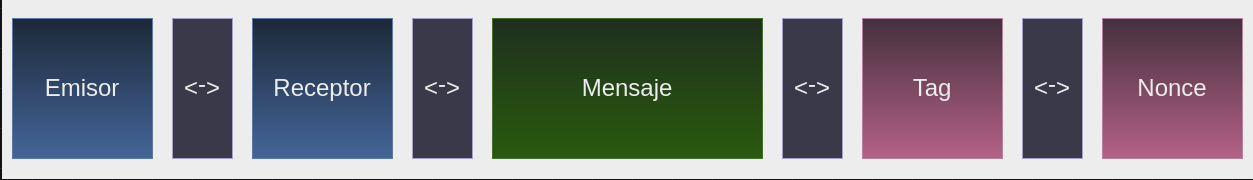
\includegraphics[width=400]{imagenes/mensaje_app.png} 
	\caption{Esquema de la codificación del mensaje.}
	\label{mensajeapp}
\end{figure}


%
\chapter{Conclusiones y trabajos futuros}

%
%\input{capitulos/06_Implementacion}
%
%\input{capitulos/07_Pruebas}
%
%\input{capitulos/08_Conclusiones}
%
%%\chapter{Conclusiones y Trabajos Futuros}
%
%

%%\nocite{*}

\bibliographystyle{plainurl}
\bibliography{bibliografia/library.bib}\addcontentsline{toc}{chapter}{Bibliografía}
%
%\appendix
%\input{apendices/manual_usuario/manual_usuario}
%%\input{apendices/paper/paper}
%\input{glosario/entradas_glosario}
% \addcontentsline{toc}{chapter}{Glosario}
% \printglossary
%\chapter*{}
%\thispagestyle{empty}

\end{document}
